\documentclass[11pt,a4paper]{report}

% Aberstwyth dissertation LaTeX Template
% Authors: Dr. Hannah Dee (hmd1@aber.ac.uk), Neil Taylor (nst@aber.ac.uk)
% This has been adapted from the Leeds Thesis template and the
% Group Project template for Computer Science in Aberystywth University.
%
% All comments and suggestions welcome.
%∫
% Template designed to be used with pdflatex: it may need alteration to
% run with a different LaTeX engine

% To build document on the unix command line, run four commands:

% pdflatex dissertation
% bibtex dissertation
% pdflatex dissertation
% pdflatex dissertation
\usepackage{listings}
\usepackage{color}
\usepackage{textcomp}
\usepackage{pgfplots}
\usepackage{booktabs}
\usepackage{pgfplotstable}
\usepackage{algorithm}
\usepackage{algpseudocode}


% you will end up with dissertation.pdf
\usepackage{mmp}

% the following packages are used for citations - You only need to include one.
%
% Use the cite package if you are using the numeric style (e.g. IEEEannot).
% Use the natbib package if you are using the author-date style (e.g. authordate2annot).
% Only use one of these and comment out the other one.
\usepackage{cite}


%\usepackage{natbib}

% Use the following to selectively exclude chapters
%\includeonly{cover,abstract,acknowledge,declare,chapter1,chapter2}

\begin{document}

% all of the include directives below refer to tex files
% so 
\title{MapMyNotes}

% Your name
\author{Ryan Gouldsmith}

% Your email
\authoremail{ryg1@aber.ac.uk}

\degreeschemecode{G401} %e.g. G400
\degreeschemetitle{Computer Science (inc Integrated Industrial and Professional Training} % e.g. Computer Science
\degreetype{BSc}

\modulecode{CS39440} % i.e. CS39440, CC39440, CS39620
\moduletitle{Major Project} % i.e. Major Project or Minor Project

\date{\today} % i.e. the date of this version of the report

\status{Release} % Use draft until you create the release version. Then, change this to Release.
\version{1.0}

%The title and name of your supervisor.
\supervisor{Dr. Hannah Dee}

%The email for your supervisor.
\supervisoremail{hmd1@aber.ac.uk}

\maketitle
 includes cover.tex - to change the content,
% edit the tex file

\pagenumbering{roman}

% This is the front page

\title{MapMyNotes}

% Your name
\author{Ryan Gouldsmith}

% Your email
\authoremail{ryg1@aber.ac.uk}

\degreeschemecode{G401} %e.g. G400
\degreeschemetitle{Computer Science (inc Integrated Industrial and Professional Training} % e.g. Computer Science
\degreetype{BSc}

\modulecode{CS39440} % i.e. CS39440, CC39440, CS39620
\moduletitle{Major Project} % i.e. Major Project or Minor Project

\date{\today} % i.e. the date of this version of the report

\status{Release} % Use draft until you create the release version. Then, change this to Release.
\version{1.0}

%The title and name of your supervisor.
\supervisor{Dr. Hannah Dee}

%The email for your supervisor.
\supervisoremail{hmd1@aber.ac.uk}

\maketitle


% Set up page numbering
\pagestyle{empty}

% declarations of originality
\thispagestyle{empty}

%%%
%%% You must sign the declaration of originality.
%%%
\begin{center}
    {\LARGE\bf Declaration of originality}
\end{center}

I confirm that:

\begin{itemize}
\item{This submission is my own work, except where
clearly indicated.}

\item{I understand that there are severe penalties for Unacceptable Academic Practice, which can lead to loss of marks or even the withholding of a degree.}

\item{I have read the regulations on Unacceptable Academic Practice from the University's Academic Quality and Records Office (AQRO) and the relevant sections of the current Student Handbook of the Department of Computer Science.}

\item{In submitting this work I understand and agree to abide by the University's regulations governing these issues.}
\end{itemize}

\vspace{2em}
Name: Ryan Gouldsmith  \\

\vspace{1em}
Date: \today \\

%%%
%%% We would like to make a selection of final reports available to students that take
%%% this module in future years. To enable us to do this, we require your consent. You
%%% are not required that you do this, but if you do give your consent, then we will have
%%% the option to select yours as one of a number of reports as examples for other
%%% students. If you would like to give your consent, then please include the following
%%% text and sign below.
%%%
%%% If you do not wish to give your consent, please remove this from your report.
%%%
\vspace{1em}
\begin{center}
    {\LARGE\bf Consent to share this work}
\end{center}

By including my name below, I hereby agree to this dissertation being made available to other
students and academic staff of the Aberystwyth Computer Science Department.

\vspace{2em}
Name: Ryan Gouldsmith  \\

\vspace{1em}
Date: \today \\


\thispagestyle{empty}

\begin{center}
    {\LARGE\bf Acknowledgements}
\end{center}

I'd like to thank my supervisor, Dr. Hannah Dee for the support received during the project especially facilitating as the customer throughout the process and the advice and direction given to improve my technical and non-technical skills. I'd also like to thank Dr. Harry Strange for suggesting the initial project title.

I am grateful to all my friends and family for their support throughout my degree. Special acknowledgments go to Laura, who has stood beside me throughout my degree. An honorable mention goes to Katie who helped in proof reading the report before submission.
 % Acknowledgements
\thispagestyle{empty}

\begin{center}
    {\LARGE\bf Abstract}
\end{center}

%Include an abstract for your project. This should be no more than 300 words.

Handwritten notes are still an important aspect of note-taking. Moving into the 21\textsuperscript{st} century, users are becoming more connected with Internet services. \textit{MapMyNotes} aims to build the bridge between handwritten notes and Internet-connected services (e.g Google Calendar events).

\textit{MapMyNotes} can be considered as three distinct sections: image pre-processing, handwriting recognition and an accompanying web application. Integrating with an Optical Character Recognition (OCR) tool, it aims to suggest metadata from the note, which aids in tagging a note. The application also integrates with the user's calendar to archive the notes.

The paper explores a variety of issues through the analysis, design, implementation and testing stages, giving justification on key design and implementation decisions. Results are presented to show the OCR's performance over a series of training examples. There are insights and thoughts concluding where the note-taking tool could then be taken further.
                 % Abstract

\pagenumbering{roman}
\pagestyle{fancy}
\fancyhead{}
\fancyfoot[C]{\thepage}
\renewcommand{\headrulewidth}{0 pt}
\renewcommand{\chaptermark}[1]{\markboth{#1}{}}


\tableofcontents
\newpage
\listoffigures
\newpage
\listoftables
\newpage

% Set up page numbering
\pagenumbering{arabic}

\setchapterheaderfooter

% include the chapters
\chapter{Background \& Objectives}

%This section should discuss your preparation for the project, including background reading, your analysis of the problem and the process or method you have followed to help structure your work.  It is likely that you will reuse part of your outline project specification, but at this point in the project you should have more to talk about.

%\textbf{Note}:

%\begin{itemize}
   %\item All of the sections and text in this example are for illustration purposes. The main Chapters are a good starting point, but the content and actual sections that you include are likely to be different.

  % \item Look at the document on the Structure of the Final Report for additional guidance.

%\end {itemize}

\section{Background}
%What was your background preparation for the project? What similar systems did you assess? What was your motivation and interest in this project?
Handwriting notes is still considered to be an important aspect of note taking. Smoker et al. \cite{citeulike:13988059} conducted a study comparing handwritten text against digital text for memory retention and out of 61 adults 72.1\% preferred to take notes using pen and paper, rather than on a computer. Smoker et al. concluded that recollection rates for handwritten text was greater than that of typed text proving that handwritten notes are better for a user's memory retention.

Technology has advanced and people are becoming more connected with distributed services through the cloud as well as tracking things in their life digitally; Google Calendar is an example of this. Therefore, there's a need to ensure that memory retention with handwritten notes is carried forward into the digital age.


% Taxonomy of notes
\subsection{Taxonomy of notes}
When notes are made they will often vary in structure from note to note. Some are semi-structured and some are ``back of the envelope'' kind of notes. When thinking about an application to analyse notes, first there has to be consideration for what a note will consist of. A taxonomy, by definition, is a biological term for a classification of similar sections, showing how things are linked together \cite{citeulike:Taxonomy}.

As an initial step in this project an informal survey of note-takers was conducted. It was concluded that notes can be thought of as a collection of similar classifications, whether this is the pure textual descriptions of a note or whether this is purely pictorial form or a mixture of both. However, the notes are normally split into three distinct categories:
\begin{enumerate}
	\item Textual descriptions
	\item Diagrams
	\item Graphs
\end{enumerate}
\begin{figure}[h!]
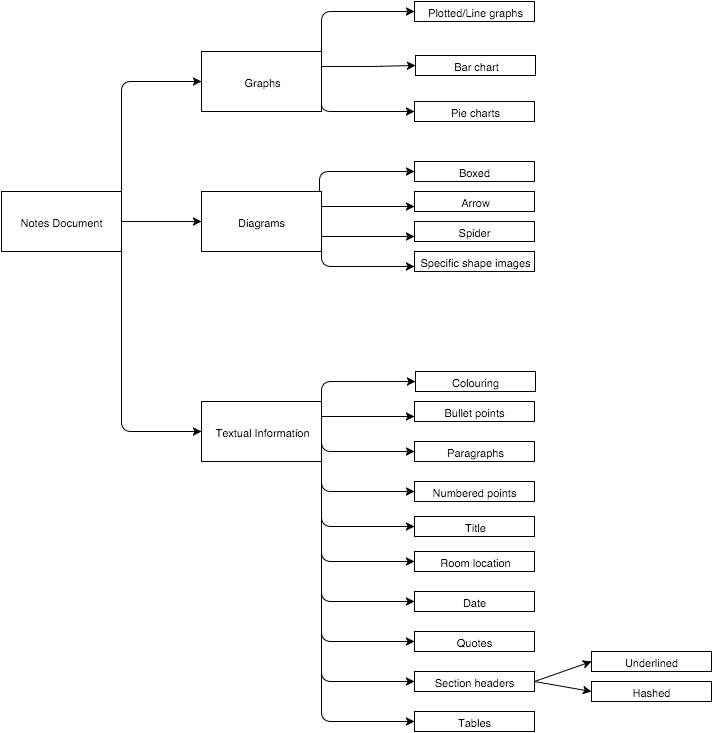
\includegraphics[scale=0.5]{images/taxonomy}
\centering
\caption{A taxonomy showing the structure and classification of different types of notes and what is contained in a note.}
 \label{fig:taxonomyofnotes}
\end{figure}

Figure \ref{fig:taxonomyofnotes} shows a taxonomy of the different aspects which may form a part of a note. Textural descriptions form the core content of a note, this is essentially the important aspect that a note-taker is trying to remember and write down. Different note-takers form their notes in different ways, for example the headings may be underlined or hashed - if they were adopting a mark-down style approach. These sections help to show that there's a break in the content, and should be sub-sectioned. Text points that are short, but important, are often characterised by a colon or a bullet point; these are the most common form of concise note building, in the classification.

Coloured text is often used for a variety of reasons: it stands out on the page and improves memory retention of that text \cite{citeulike:14014177}. Both congruent and incongruent  coloured text helped to increase memory retention of post-graduate learners \cite{Olurinola_Tayo_2015}. With congruent text, Olurinola et al. showed that for 30 students with a 20 word list, a 10.9 mean retention rate was achieved and a 8.1 mean retention rate was achieved for incongruent text. The studies conducted show that coloured items would improve a user's retention rate in a lecture.

Finally, tables help to represent textual content in tabular form - this is often good in notes for comparisons.

Graphs are great visual tools for users to help to convey important textural information easily. Naturally, they have their limitations such as they come in different shapes and sizes, such as a line-graph, pie chart or a bar chart. Coupled with graphs, notes often consist of diagram drawings.  In Figure \ref{fig:taxonomyofnotes}, there are different sections and classifications of a diagram: boxed, arrow etc. Each one has its own purpose and arrowed and box can overlap; UML diagrams are a case of this. Spider diagrams are probably the hardest to represent, due to the varying sizes and whether the user draws circles or clouds. Furthermore, specific shape diagrams are conceptually hard to think about as it depends on the domain in which the user is drawing the note. For example, a person in Biology may draw a stick person, whereas someone in Computer Science may draw a computer.

Identifying a taxonomy of notes is imperative when considering what to parse from a note as it helps to define a domain of possible classifications. By identifying the classifications it will acknowledge what sections can be parsed by a specific technique. For example, textural information and bullet point lists can be parsed via text-recognition however, for diagram recognition that would involve image manipulation.

% Add some more from the stuff Hannah made us write about in the first week.

% Handwriting triaining ?
\subsection{Handwriting recognition}
Analysing a user's handwriting is a complex process and one which requires lots of research. Handwriting recognition has had successes in the past from machine learning techniques, such as neural networks \cite{citeulike:13510433}. Knerr et al. yields a 10\% rejection rate and  a 1\% error rate, with the use of Neural Networks on the U.S. Postal service data collection, showing that handwriting recognition is still very much an active research area, where solutions are still being developed to optimise the correct classifications of text.

Another approach is to analyse handwriting via an OCR (optical character recognition) tool. Rakshit et al. \cite{citeulike:13920972} used the open-source tool, Tesseract \cite{citeulike:14014368} to analyse Roman scripts. The system was trained on handwriting identified from those scripts. Rakshit et al. recorded an 83.5\% accuracy on 1133 characters. It is noted in the paper that ``over-segmentation'' is a problem with the Tesseract engine.

Another issue to overcome when analysing handwriting is disjointed characters; this is where sections of the letter are split off from the main body of the character, for example, the letter i. Rakshit et al. concludes that this is an issue which is ever-present in the Tesseract engine, with around a 53\% misclassification rate on this character alone.

The problem of handwriting recognition has not been solved - but tools such as Tesseract offer support for improvement in this field. As Rakshit et al., discussed training had to be conducted with Tesseract to ensure that it can identify handwriting successfully. As a result, every implementation of handwriting recognition needs significant amounts of data of varying quality, so that a system can succeed. However, considering Tesseract's high text identification rate of 83.5\% experienced by Rakshit et al., it is a viable option to use for handwriting recognition.

\subsubsection{How Tesseract works}
Tesseract was initially developed by HP, but has now been made into an open-source tool. Ray Smith \cite{33418} gives an excellent overview of the Tesseract engine, the following section summaries how Tesseract works. Tesseract uses connected components to identify the outline of characters, these are then collated into blobs. These blobs are then collected into text lines, which are deconstructed into individual words.

The process then goes through a two stage process, of identifying the words first - and the second identifies words which are not well known. Tesseract has the ability to identify textlines from skewed images \cite{citeulike:14024253}. Therefore, as long as the image is text, a slight skewing of the image would not affect the ability to identify text. Textlines are found from the blobs, filtered and then sorted aided for tracking. Blobs are then processed in order checking for overlapping coordinates - from which they're either added to a new line, or appended to an existing line.

Smith discusses that the words are then split into characters. Due to handwritten text being varied, as a user would not write uniformly, then chopping is complex.

After the word has been chopped Tesseract needs to segment the character to identify the character. Smith describes that chopping may leave parts of the characters unattached, so an A* algorithm is used to compare different fragments from a graph of chopped characters. These broken characters are then checked against previously trained examples and similar patterns are attempted to be extracted.

The classification is described by Smith as a ``two step process''. Firstly, the character is evaluated and matched against a potential list of characters from previous examples. The second step involves calculating how well that character matches those in the list, the highest match is then selected as the character.

It is important to acknowledge that Smith discusses the implementations of Tesseract as a whole, with results comparable for printed text, not handwritten text - where there is more variation. However, the paper gives a detailed explanation of the complex process of how Tesseract analyses the image, as well as the text.

\subsection{Similar systems}
With note-taking on digital devices becoming more widely available, there has become an influx in note-taking and organisational applications available for users. These are predominately WYSIWYG (what you see is what you get) editors - which allow a great deal of flexibility. When evaluating existing systems three were predominantly used and they were:
\begin{itemize}
  \item OneNote
  \item EverNote
  \item Google Keep
\end{itemize}

\subsubsection{OneNote}
OneNote \cite{citeulike:onenote} is a note-taking and organisational application made by Microsoft, offering the functionality to add text, photos, drag and drop photos onto a plain canvas. In recent times, OneNote has developed functionality to analyse a user's handwriting, from say a stylus, and interpret the text they entered \cite{citeulike:14014236}. In OneNote you can insert a note into a document and then it would interpret the text from the note.

There is a wide range of product support from mobile based applications to web versions of their software. Office Lens \cite{citeulike:14014272} can be used in conjunction with the OneNote to help to take photos and automatically crop the image and then save them to OneNote. This feature is important and should be considered for the \textit{MapMyNotes} application. The process requires the user to sign in with  a Microsoft account. When creating notes, OneNote formats collated notes into a series of ``notebooks''.

One feature which was noted when analysing the system is automatic saving of the note, reducing the need for a user to click save. Additionally, when using OneNote it feels very much like Microsoft Word - with the similar layout that gives most users a similar user experience feel with its intuitive WYSIWYG editor.

\subsubsection{EverNote}
EverNote \cite{citeulike:14014282} is a note-taking and organisional application, it is supported as a web application, bespoke desktop application and a mobile application. EverNote is widely used and provides a wide range of functionality a user would need to digitise their notes.

EverNote have released development articles \cite{citeulike:13988110} stating that OCR recognition on images is possible. This would allow the user to upload an image outputting a list of potential words for each word found in the image. Like OneNote, the notes are collated into Notebooks, offering a WYSIWG editor, giving the user full control of the content that is entered. When uploading an image to the web version it gives the option to edit the PDF and images, however it seems as though an additional application has to be downloaded, specific to the user's platform, to be able to utilise this functionality.

According to the website, it does do OCR recognition, however whilst using the web application there was no information regarding extracting of text from the application. Additionally, there seemed to be no way to save the note to a calendar item - only the option to send via a link.

\subsubsection{Google Keep}
Google Keep \cite{citeulike:14014320} is a note taking application produced by Google with mobile and website support. Google Keep allows a user to attach an image to their note, attempt to extract the text from an image and save this in the body of the note. In addition it allows the user to tag a title and add an associated body.

An important design feature that it does not offer is the support of a WYSIWG editor; a default text box has been preferred, offering a more raw feel to the application. They have the option of a ``remind me'' feature, which will get synced to their calendar as a reminder - but there's no easy way to add it to a calendar event.

Google Keep seems as though it's more suited for TODO lists and jotting down quick notes, rather than an archiving tool suitable for substantial note taking. Nevertheless, the tagging with labels is a nice feature and the filter by image is a smart tool; this only shows notes with specific images. The simplicity of the User Interface (UI) and the ease in which text can be extract provides a great reference.

\subsubsection{Reflection on the systems}
These three existing products are widely used by the every day note-taker. They have been developed to a high quality and give the user full control of what their notes can consist of. The automatically cropping of an image is an important feature and should be considered  for the application in the future. \textit{MapMyNotes} aims to try and give the user full control of their lecture notes content, so that they can find their notes easily.

\textit{MapMyNotes} intends to differ from EverNote's text extraction by providing a one to one comparison of the text, rather than a list of potential words.

After the analysis of the existing products there are certain aspects which would be regarded as necessary: a simple way to view the notes, a way to filter the notes and a simple UI which feels more like an application rather than a website.


\subsection{Motivation}
The author handwrites his notes during lectures and these are often stored in notebooks, with no structure ,until they are needed for an assignment or examination.

A calendar event is already stored for every lecture that the author goes to, so it would be useful if there was a way to associate each of the notes taken to that calendar event. This would ensure that all the information is located in one easy place that can be found, instead of trawling through lots of paper and trying to find the content. This would aid in reducing the chances of lost notes from paper slipping out of the notebook or pages being damaged due to rain or creases.

\section{Analysis}
%Taking into account the problem and what you learned from the background work, what was your analysis of the problem? How did your analysis help to decompose the problem into the main tasks that you would undertake? Were there alternative approaches? Why did you choose one approach compared to the alternatives?

%In most cases, the agreed objectives or requirements will be the result of a compromise between what would ideally have been produced and what was felt to be possible in the time available. A discussion of the process of arriving at the final list is usually appropriate.
As the project was originally proposed by Dr Harry Strange, a meeting was arranged to discuss the initial ideas that he wished the application would follow. It was here that it was highlighted that Dr Harry Strange wants to take a photo of his notes, archive them with specific data, make them searchable and integrate them with existing calendar entries he had for a given date.

\noindent
\textbf{Parsing a note}


In conjunction with the information gathered a taxonomy of notes was collated, helping to deconstruct what a note consists of. Analysing the taxonomy produced a comprehensive breakdown of what could be parsed as text. After seeing that text formed the main component of the note the primary efforts of the application would be focussed on parsing the text. Diagrams, graphs and image would be future work - due to time constraints.

\noindent
\textbf{An OCR tool}


Handwriting recognition has been an active research project for a while. There could have been the possibility of creating a bespoke handwriting recognition tool, using machine learning techniques, but that would distract from the actual problem which is this available tool to archive notes.

Therefore an OCR tool would have to be chosen to analyse the text. Choosing a sensible OCR tool with good recognition rates would be important - so a task was created to explore and look at possible solutions.

\noindent
\textbf{What to parse from the note}


From research conducted into Google Keep it was clear that analysing the text would be a great aspect to include in the application. The real question is what should be parsed from the note? By looking at the overall structure of the application and what it entailed then it was agreed to just parse the note's associated metadata: the title, lecturer, date and module code. Recalling that Google Keep parses all the text and EverNote gives a list of suggested words, it was decided that a tool would be developed to suggest the metadata but not automatically tag the metadata.

\noindent
\textbf{Structuring of notes}


In conjunction with analysing what to parse, a sensible structure would have to be applied to notes used in the application. A task to create and find a good set of rules would have to be collated to ensure that notes could be parsed confidently. This reduced the complexity of incorporating natural language processing in the application, which would be implausible to be completed within the timeframe.

\noindent
\textbf{OCR for the authors handwriting}


After research into OCR technologies, such as Tesseract \cite{citeulike:14014368}, it was established that analysing handwriting is a complicated process. Instead of trying to train it on a lot of dummy data, it would be trained to recognise the author's handwriting. A task was created to train the user's handwriting data and this would run throughout the duration of the project.


\noindent
\textbf{What platform is most suitable}


During the meeting with Dr Harry Strange one of the core features that was needed was for the application to be accessible regardless of where the user is. After the research was conducted all the aforementioned software tools have a web application version of their system. A mobile application was considered but only one version of the application would be made, either Android or iPhone, therefore preventing other phone users from using the application. A bespoke desktop application was considered for a long time, however, the user would have to ensure infrastructure decisions, such as databases, are correctly set up. As a result a web application was chosen - following research found; the next steps were to consider appropriate tools to use.

\noindent
\textbf{What should the application do}


From analysing all three of the chosen research systems, it was clearly identifiable that they all have the ability the view all notes, searching, deleting, adding and editing a note. Taking these ideas on-board, they were set as a high-level task and something that the core system \textit{must} do.

Reflecting on the premise of the application, that it was to aid the organisation of lecture notes, it was concluded that the best way to search for notes would be by module code, as most University students would want to find specific module notes. This created the high level task that notes must be searchable by their module code.

\noindent
\textbf{Calendar integration}


From evaluating the systems it was noticed that there was not a clear way to integrate into a calendar. Reflecting on the conversations with Dr Harry Strange, integrating with the calendar was important for keeping the different systems together. From an AYTM survey, in December 2015, \cite{citeulike:14010520} Google calendar is the most popular calendar application, therefore due to time constraints Google calendar was the choice of integration and other competitors such as Microsoft would not be implemented. This formulates the task of integrating the calendar into the application to save the url of the note to a specific event.

%There should be a clear statement of the objectives of the work, which you will evaluate at the end of the work.
\subsection{Objectives} \label{analysis:requirements}
As a result of the analysis of the problem, the following high-level requirements were formulated:
\begin{enumerate}
	\item Investigate how to extract handwriting text from an image - this will involve looking into ways OCR tools can interpret handwriting.
	\item Train the OCR to recognise text of the author's handwriting.
	\item Produce a set of a rules which a note must comply to.
	\item Produce a web application to form the core part of the product. This includes allowing a user to upload an image, display the image. Add appropriate tagging to a note such as module code.
	\item The user must be able to search for a given module code, showing the fill list of notes based on the module code entered.
	\item The backend of the application must conduct basic OCR recognition, analysing the first 3 lines of the notes.
	\item The backend must integrate with a calendar to archive the notes away later to be found again.
\end{enumerate}

\subsection{Compromising with objectives}
Some additional compromises were made separate of the analysis due to the complexity of the tasks at hand.
\begin{itemize}
	\item It would be nice to have image extraction from a note and incorporating a WYSIWG editor into the application, like OneNote.
	\item Full OCR on all the characters. This would then output the text to a blank canvas.
	\item Make the handwriting training generic enough to identify a wide range of users handwriting.
\end{itemize}

It is worth noting down that the project supervisor Dr Hannah Dee felt as though the handwriting training would be too much for the dissertation and should be done as a ``maybe''. After much deliberation it was decided to include it, but as a background process.

\section{Process}
%You need to describe briefly the life cycle model or research method that you used. You do not need to write about all of the different process models that you are aware of. Focus on the process model that you have used. It is possible that you needed to adapt an existing process model to suit your project; clearly identify what you used and how you adapted it for your needs.
Software projects often have a degree of uncertainty with requirements at the beginning, these projects lend themselves to an Agile approach. More structured applications with requirements which are well known are suited to a plan-driven approach.

For this project there are a lot of tasks which are not 100\% definable at the start of the project. In addition to this certain tasks, such as training the author's handwriting data, can not be truly estimated down to a fixed time. Often new requirements would emerge from weekly meetings and only high level requirements were in-place from the start of the project. As a result, a plan-driven approach such as the Waterfall model would not be appropriate, and an Agile methodology was implemented.

\subsection{Scrum overview}
Scrum \cite{citeulike:14014350} is a methodology used by teams to improve productivity where possible. Due to this being a single person project, a Scrum approach has to be modified. Sprints are set time-boxes where tasks are completed. These vary from one to four weeks in length but a shorter sprint means the developer can act on quicker feedback.

Scrum organises its work into ``user stories'' to ensure client valued work is being completed. They are normally collected at the start of the project and put into the backlog, which is a collection of client valued work. At the start of each sprint user stories are selected from the backlog with an estimation on complexity performed. Finally, at the end of the sprint a review and retrospective is conducted to analyse the sprint, identifying what went well and what could be improved.

\subsection{Adapted Scrum}
During the project this methodology was embraced and adapted. A one week long sprint was adopted which coincided with a weekly supervisor meeting. Epics (a high level version of a story) were identified at the start of the project to reflect the work completed in the analysis phase.

The epic was then broken down into user stories. Each user story was formulated as: ``As a \textless role\textgreater I want to \textless feature\textgreater so that \textless resolution\textgreater''. This gave specific client value that was known to have a purpose. Each of these stories were estimated on their complexity and compared to a ``goldilocks'' task \footnote{A task which all other tasks are evaluated against.}.

For planning a sprint, the planning poker \cite{citeulike:14014357} technique was adopted; user-stories are estimated on a scale of 1, 2, 3, 5, 8 etc. When a task was estimated about 15 story points, it would be reflected upon to ensure the scope was fully understood - this would be broken down to sub-stories where appropriate.

At the end of a sprint a review and retrospective was conducted in the form of a blog post \cite{citeulike:14014367}, instead of in a team. The retrospective was used to analyse what was achieved in the sprint, what went well and what needed to be improved upon. During this time, pre-planning was conducted to formulate a series of tasks to complete in the next sprint; this was agreed by the customer (Dr Hannah Dee).

Communication with the project supervisor was key to determine what needed to be completed. It was discussed if what was suggested was achievable in that weeks sprint, based on the total story points completed in the previous sprint; if 20 story points were completed in sprint 3 then 20 story points were estimated for sprint 4 - associated user stories were brought forward.

The project was managed on the open source management tool Taiga.io \cite{citeulike:14014360} which was invaluable, and provided built in functionality such as burndown charts per sprint. This shows how well story points are being completed, in the form of velocity, and are used as an analytical tool for how well progression was being made.

Daily stand-ups were informally conducted with a peer. Cut from the usual 15 minutes to around 5 minutes, the conversation helped to identify if there were any issues, what had been completed yesterday and what would be completed that day. Peers aided to listen to This provided a good way to analyse what needed to be achieved and keep in perspective how the sprint was going. This was reciprocated from both sides where both Major Projects were discussed. The primary aim was to identify the main tasks which needed to be completed that day to keep the project moving forward.

\subsection{Incorporated Extreme Programming}
In tandem with Scrum, Extreme programming \cite{citeulike:13915786} principles were integrated into the development process; merciless refactoring, continuous integration and test-driven development were borrowed from its principles.

\subsubsection{Test-driven development}
Test-driven development (TDD) is the process of writing tests prior to the implemented code. This allows the developer to think about the design prior to its implementation and can form part of the documentation \cite{citeulike:14014361}. This was implemented throughout the project, with both unit and acceptance tests being written before the code implementation.

TDD follows three cycles: red, green, refactor. Initially the test fails, then it passes then refactoring is performed to keep the simplest system.

\subsubsection{Continuous Integration}
Continuous Integration tools were a core part of the process in this project. Typically used to ensure that code is checked into a repository it was used to ensure that the application could be built in an isolated environment and pass all the tests. This would result in ensuring that new features were created from all code committed into the repository. See Section \ref{tools:CI} for further reference on how CI was used in the project.

\subsubsection{CRC cards}
Class, responsibilities and collaboration (CRC) cards \cite{citeulike:13398676} were used during the design section to consider how different classes were to be created and the responsibilities they share. This principle from Extreme Programming helped to keep the design simple and not convoluted. See Section \ref{design:CRC} for further reference on how CRC cards were utilised.

%\addcontentsline{toc}{chapter}{Development Process}
\chapter{Design}

%You should concentrate on the more important aspects of the design. It is essential that an overview is presented before going into detail. As well as describing the design adopted it must also explain what other designs were considered and why they were rejected.

%The design should describe what you expected to do, and might also explain areas that you had to revise after some investigation.

%Typically, for an object-oriented design, the discussion will focus on the choice of objects and classes and the allocation of methods to classes. The use made of reusable components should be described and their source referenced. Particularly important decisions concerning data structures usually affect the architecture of a system and so should be described here.

%How much material you include on detailed design and implementation will depend very much on the nature of the project. It should not be padded out. Think about the significant aspects of your system. For example, describe the design of the user interface if it is a critical aspect of your system, or provide detail about methods and data structures that are not trivial. Do not spend time on long lists of trivial items and repetitive descriptions. If in doubt about what is appropriate, speak to your supervisor.

%You should also identify any support tools that you used. You should discuss your choice of implementation tools - programming language, compilers, database management system, program development environment, etc.

%Some example sub-sections may be as follows, but the specific sections are for you to define.

As the application was developed in an iterative manner, over a series of sprints, class diagrams and design diagrams were not created at the very start of the project. Over a series of sprints designs were iteratively developed regarding the system overview. However, some design decisions were decided at the start of the project. The chapter will clearly explain rationale for the decisions and state whether the design decisions were a result of iterative processes or upfront design.

\section{Implementation tools}
The following discusses the design decisions regarding the implementation tools that were used during the project, providing rationale for the choice of tools.
\subsection{Programming language}
With the programming language choice unlikely to change per sprint, then an upfront design decision was made. From the analysis it was concluded that the application would be implemented as a web application.  A consideration between different server side programming languages was considered in depth.

Typically with server side applications the traditional language choices are: PHP, Ruby, Python, C#, Java and JavaScript, which has increased in popularity recently \cite{citeulike:14018462}.

Evaluating the analysis decomposition in the meetings in the beginning sprints it was determined that OpenCV, would be needed to be utilised in the project. OpenCV's original source code is written in C++, however Python and Java bindings to OpenCV are available. Additional research was conducted to see if a reliable wrapper for either PHP or Ruby was available, and after a lot of investigation it was concluded there was not.

C++ is not considered a standard web application development language, therefore reducing the opportunity for support during the project, it was dismissed as viable choice. Java applications are predominately large commercial applications, using a range of enterprise software - often renowned for their performance abilities \cite{citeulike:14019744}. This approach felt too cumbersome for a proposed light-weight application.

By being constrained by design decision to use OpenCV coupled with the lack of reliable wrappers for other languages and a reluctance to use Java then Python was selected as the most suitable language. Python offers a lightweight and quick to learn syntax that produces readable code whilst allowing a object-oriented paradigm to be followed. Additionally, its support for OpenCV is sufficient for the application.


\subsection{Choice of framework}
To recap, Python was chosen as the language of choice for the application. Frameworks aid in the development of a project, especially with web applications where routing is often required; often routing support is a key feature of frameworks. Exploratory work was completed in the early sprints to find a suitable tool. The frameworks Django \cite{citeulike:14019784}, Flask \cite{citeulike:13160396} and Bottle \cite{citeulike:14019792} were evaluated.

Some frameworks constrain the developer's to specific implementations through abstracted classes whereas some offer more flexibility. Whilst evaluating Django, a full framework, it was concluded that such a large framework was excessive for this application and rejected as a choice for the framework.

Flask and Bottle are classified as ``micro-frameworks'', offering a lot less restrictive structure and allowing the developers to have more control on how the applications are structured. On face value, Flask and Bottle appear to be very similar: they are both lightweight with a similar syntax. Evaluating both of the frameworks identified that Flask had a larger support community than Flask, coupled with better documentation, compared to Bottle. As neither framework had been used before then a support community was an important design decision.

As a result, Flask was chosen as the framework which will be used throughout the application. Spike work was completed to see how simple it was to create a quick application, after discovering it was perfectly fine, Flask was agreed as the framework of choice.

\subsection{Database management system}
As the analysis suggested it should be a web application then data persistence should be an integral part of the application. Prior to choosing an appropriate tool, a rationalised decision had to be made on the different management systems available.

\subsubsection{NoSQL or relational database management systems}
The choice of database management system was considered at length. Firstly, the decision of whether to use NoSQL or a relational database management system (RDBMS) had to be decided. This was decided during the early sprints, whilst the design was beginning to emerge.

RDBMS's are suited to separating the data into logical relations which decouples through the process of normalisation. The data normally suited to a RDBMS is one which has a uniform structure and can be represented as a series of relations, with specific constraints.

NoSQL provides a more flexible structure, allowing data to have no specific structure. In MongoDB \cite{citeulike:14019766} documents are equivalent to relations - structuring the data as key-valued pairs over specific column structures. This offers more flexibility in the data passed to the database.

From previous design choices made in prior sprints regarding the database structure, both options were seriously considered. After the analysis of what the note meta data would consist of, it was decided that the structure for the data would not vary, each note will have an associated lecturer, title etc, then a relational database would be suitable for the application. In addition, the notes \textit{must} follow a specific layout structure, therefore affirming that data would be linked and structured.

A specific choice of RDBMS had to be chosen as an appropriate tool to persist the data from a note; digital ocean offered a concise comparison aiding in the design \cite{citeulike:14019772}.
\subsubsection{SQLLite}
SQLLite was considered as a viable option; Flask provides documentation for its ease of use with the micro-framework. Considering the larger picture: would it scale well with multiple users interacting with it? Digital ocean state it would be a perfectly fine testing and development tool, but for production it may not scale well with multiple reads and writes.
\subsubsection{PostgreSQL}
Digital ocean describe PostgreSQL as the most advanced of the RDBMS's available. The additional support of more types an attribute can have allows for a greater control when creating a database. For example, the JSON type support would allow the application to save returned JSON from 3rd party services directly to the database.
\subsubsection{MySQL}
MySQL and PostgreSQL for most applications would be interchangeable. It offers a wide range of support along with comprehensive documentation. There are concerns over performance, however.

\noindent
After evaluating the possible RDBMS's it was concluded that MySQL and PostgresSQL would be more preferable for scalability. Although there is not a great difference between the two, PostgreSQL was chosen for its advanced ability allowing for the application to become more advanced. This goes against the YAGNI (you ain't gonna need it) approach, but infrastructure decisions are harder to change, than code implementations.



\subsection{Continuous Integration tool}
Although Continuous Integration (CI) is normally used for development teams to ensure that all code is checked into the repository[cite], there was value in using it for a single person project. Prodomently for the build processes on the branches to ensure that the application builds in an isolated enviornment.

Having used Jenkins CI before [CITE] this was my immediate choice when considering what to use for a continous integration tool. However, whilst considering the posibilities on how to integrate this to the application I discovered the CI tool, Travis CI. This CI tool seemed easy to set up: you link it to the repository, add a travis.yml file (with configurations) and it will run and build the application. This then gives useful messages such as passing, errors or failing.

One key decision whilst considering CI tools was to show be able to check the build process whereever I am. After finding out the Travis CI is in the cloud and links directly with the GitHub repo I opted to use Travis CI for the project.


\section{Overall Architecture}

\subsection{CRC cards}
To recap, Extreme Programming uses the concept of CRC cards to help to aid the developer to think about the design of the application. Unlike UML, they are throw-away cards which can be edited and changed every time a new feature is implemented. The CRC cards which have been drawn up in the application have been formalised, and a selection of the interesting design decisions and justifications are stated below.

\begin{figure}[h]
  \centering
  \includegraphics[scale=0.5]{images/CRC_card}
  \caption{An example from Sprint 3, showing a CRC card at the very beginning of creation.}
  \label{fig:crc1}
\end{figure}

These little design diagram cards helped to consider the design of the system by decomposing the problem into more logical steps. For example, when creating the note CRC there could have been a time in which a separate class was made for the image link - however a simple design was ensured with a reflection on the card.

\subsection{Class Diagram}

\begin{itemize}
  \item Use of service objects
  \item Explain why sections are linked together and describe the behaviour of the application classes and why they would be used.
  \item
\end{itemize}

\subsection{Database diagram}
Coupled with the CRC cards a database UML diagram has been produced which shows the implementation of the relations in the database.

\begin{figure}[h]
  \centering
  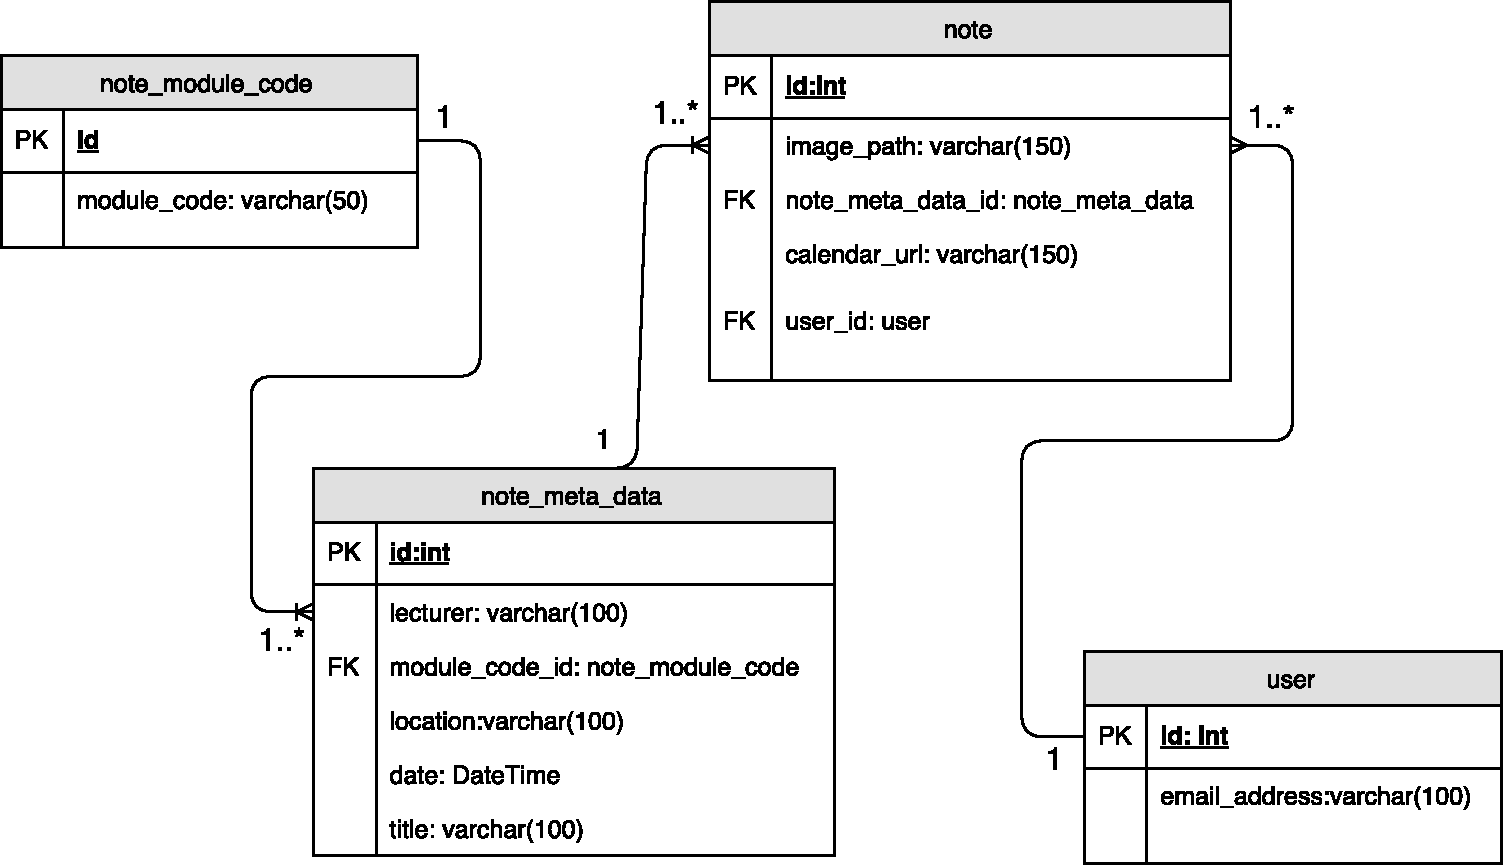
\includegraphics[scale=0.5]{images/database_diagram}
  \caption{The final result of the database diagram. After a series of iterations.}
  \label{fig:database}
\end{figure}

Figure \ref{fig:database}, shows the output from the result of continuous design on the database diagram through the iterations.

\subsubsection{Justification of design}
The design has been carefully considered. The reason the note is in its table is intuitive: a note needs to be persisted in the database. The attributes best collate a high-level representation of what a note consists of. First and foremost,  a note will consist of an image link - which is a relative path, this was stored to persist where the image on the file store is located for that image. A user id was added to the note, to link a note to a user; not originally in the scope of the application, but a design feature added so that it was more accessible.

The calendar url was added to the database to persist which calendar event was associated with the note. As a note will only have one calendar event, then saving it in the database was an easier way to link to the event - rather than making an external API request to Google.

Finally with the note relation, a note-meta-data foreign key id was added to link additional note-meta-data to a note.

The Note-meta data relation is its own relation because of reducing data-redundancy, this is a key requirement in normalisation of databases [CITE]. The note Meta-data may be duplicated in a note if a user takes more than one note per lecturer - and wants to tag the same meta-data to the note. As a result a relation was created for this use-case.

The meta-data consists of a lecturer, location, and title as variable characters up to 100 in length, which is a valid length as none of them realistically should be more than that length. A date field was added so the meta-data can be associated to a date and time - this aids in the calendar integration. Finally, the module code is identified as a foreign key constraint.

The module code is its own relation, and therefore a foreign key in the meta-data relation is because of the same reasons as meta-data is it's own relation: data redundancy. A valid use-case is that a user would enter in multiple notes for any given module code. This module code does not need to be duplicated in the database - therefore a foreign key was suitable.

Finally, a user relation was established after the application decided it would be expanded to involve users. An email address was created to parse the response from the oAuth log-in. Furthermore, this was added as a foreign key to notes, so that every user would be associated to a note.

Overall, a succinct collection of relations have been developed, which follow a good normalization process to produce a design from a database side which has been well considered.

%\section{Some detailed design}


\subsection{MVC Structure}
Early on in the process it was decided that an MVC approach would be approached. This was an upfront design decision, that would not likely to be changed.

\subsubsection{About MVC}
MVC is a design pattern where you split the logic into a Model View and controller. As displayed in figure \ref{fig:mvc} the MVC approach helps to decouple logic from the view file. Therefore all the information passed to the view is renderable content. The controllers do not integrate with the database directly. The primary job for the controllers is to interact with the model, any services and ask to render the view files.

The model in the MVC structure has no acknowledgement of the view file. Instead of rendering any form of HTML in the model it is purely data-driven. The sole purpose of the model is to interact with the database and perform any business logic that does not fit in the controller and the view file.

Finally, the view files contain HTML logic with dynamic content passed to the file from the controller. There may be specific logic which impact the HTML displayed, but no direct calls are made to the database layer or the controller. It uses the dynamic content passed in.
\begin{figure}[h]
  \centering
  \includegraphics[scale=0.5]{images/MVC}
  \caption{A example of how the model-view-controller(MVC) framework integrates.}
  \label{fig:mvc}
\end{figure}

\subsubsection{Structuring the Web application}
The application was chosen to follow the MVC approach so that there was a clear distinct design pattern used, which did not obfuscate where logic and presentation layers interact. With a well structured system it makes testing easier.

In addition to the structuring, components can be reused again easily. Take for example service classes, these are reusable components in the system where they can be easily instantiated from inside any controller. If an MVC approach was suggested for the design then the reusability of code would decrease. This could only be achieved from a nice decoupled system where independent logic can be processed separately.

Although the MVC approach was desired, Flask does not support an MVC structure out of the box. During a lot the documentation it expects all routes to be placed in a single file. This design approach was not considered for a number of reasons: it reduces the readability of the code - if there is more than one class per file, then readability begins to be impacted. Furthermore, when considering the design of the controller objects, as well as the models, then dependencies between the classes would become obfuscated. From identifying an architecture perspective, if the routes were on one file and models in another, it would be hard to explicitly identify corresponding links between different files.

To overcome the Flask routing issue, in recent versions [FIND VERSION NUMBER] Blueprints [CITE] have been included. These blueprints, act almost as controller files, like Ruby, using the routing annotation to create a route. Therefore, similar routes can be place in the same file, but a different file can be created for unrelated routes. This offers a good controller feel to the application.

The models consist of both persistence logic as well as service and helper objects. All the business logic is kept in side this group. Finally, all the views are allocated to the view directory.

\subsubsection{Extending views}
It is worth mentioning that Flask uses the Jinga templating engine[CITE]. By default Jinga would expect the DOM to be represented again in every view file. A design decision was made to extend the view files. Figure \ref{fig:extension} illustrates the view file design.
\begin{figure}[h]
  \centering
  \includegraphics[scale=0.5]{images/view_file_extension}
  \caption{A diagram illustrating how extension in Jinga html template engine works.}
  \label{fig:extension}
\end{figure}

Each of the view file templates are separated into their own directories. Inside the directories, the HTML files extend the index.html root file. This overrides the block ``content'', dynamically generating a new content for every new URL. The advantages of this design is that meta-data, headers, stylesheets and navigation can be placed in the index.html page and all subpages will inherit these automatically, sticking to the principle of DRY.

\subsection{Application URLs}
When considering the application URLs would form an integral part of helping the users to identify where they are, what the page is aiming to achieve and, where applicable, bookmarkable.

Therefore designs into the URL structure was performed. Typically there are two types of URL structures which websites take: query strings or REST URLs.

Query strings aid in the creation of URLs such as: /search?name=foo. The query string is represented as a key value pairing of the searched criteria. This form of URL representation is acceptable for search criteria, but what if the user was editing a note - would a good structure contain all the contents of that note?

For parts of the application to overcome this issue REST [CITE] URLs were considered. By exposing the URLs to RESTful interface, it is clear what the application is intending to do on that page. For example $/show_note/1$ compared to $/show_note?note_id=1$. Therefore, the URLS will follow a hierarchal structure, showing exactly where the notes are, in this case [CITE].

It is worth noting that RESTful URLS are a good concept for external API usage. However, due to the application being a web application some modifications were taken place. For example, the URL: $/view_notes/$ would be a better RESTful url as /notes/. However, the design decision was to adopt the RESTful pattern to help make the URLs a bit more readable, but still keep the principles of REST.

\subsection{HTTP methods}
Flask supports all the REST HTTP methods, such as delete, put and patch[CITE]. However, normal web browsers have this common issue where they do not support them and instead only support GET and POST.

As a comparison in Ruby, the templating language - embedded ruby - allows being able to fake certain methods on forms and submit buttons. Unlike Flask, who uses pure HTML templates, with the Jinga syntax added on top, then developers are restricted to the default GET and POST.

Another layer of code could have been added in the form of posting everything to the URL routes on the server as AJAX requests - but that would first and foremost change the entire structure of the application. This would mean that a user would have to have Javascript enabled on the page to even interact with the application.

As a result, the design decision to use default POST and GET requests was decided. DELETE would not be used for deleting content from the database.

\subsection{Interaction with the application}
When decomposing a problem it is useful to identify how a user would intend to interact with the system.




%\subsection{Even more detail}

\section{User Interface}
Although the application was developed in an iterative approach, wiremocks were completed when UI changes occurred so that I could reflect on them.

To begin with the user interface (UI) went through a few iterations of wiremocks to sketch out what it should look like.  This iterative approach was applied when actually designing the website. Firstly it was important that the application felt as thought it was an application, rather than a traditional website. Colours from Google Style guide [CITE] was used to keep with nice, clean and bold colours. Bootstrap[CITE] was considered to be used on the application and it did give a default responsive theme built in - however, keeping with the idea of minimalist and not over-bloated, then personally I feel that that bootstrap comes with a lot of the additional material which would not be needed.

With this being a web application, a responsive navigation was always important. A user may take a photo of their note and then upload this to the website off their mobile. This resulted in the web application having to be thought about from a responsive view. I should have done this better and considered this from the beginning and built up from the responsive to the desktop version. However, I did retrospective responsive design and performed media-queries when I needed to.
% add in code examples for media query\
\begin{itemize}
  \item Wiremock examples
  \item Media query code examples.
\end{itemize}
% Include wiremocks
\section{Other relevant sections}
\begin{itemize}
  \item Why did I use a Calendar Item class to story the class and then format the date from that instance.
  \item Why Parsing the notes returned the first 3 lines. Why did this have to be done?

\end{itemize}

\subsection{Tesseract}
Comparisons between different OCR tools was researched. Evaluations into systems which would be a suitable aid was undertaken. [CITE - Case study] performs a case study using Tesseract as their OCR tool to analyse printed text in an image. Patel et al, also discuss the comparison against a proprietary OCR tool, Transym [CITE].

The results concluded by Patel et al is that Transym only yielded a 47\% accuracy on 20 images compared to 70\% accuracy using the Tesseract engine.

Analysing the outputs concluded that Tesseract would be the best performing on an image. Tesseract was chosen for its open source and it's highly commended recognition rate as well as my supervisor echoing the compliments of Tesseract and it should be considered.

\section{Optimising tesseract}

\subsection{ImageMagick}
Once Tesseract was chosen as the OCR tool training was started promptly. Due to there not being a formal way images were supposed to be prepared for the tool then the first few iterations were converted to grayscale using ImageMagick [CITE]. This yielded a poor return rate and characters were not identified consistently.

At this point in the design, the notes were being written on original lined paper. Research work was looked into to try and get the image as clean as it could be for the Tesseract engine. This resulted in monochrome from ImageMagick to be used; an increase in recognition rate was received, however the image was very messy with pixels from the lines obfuscating the response from Tesseract.

\subsection{OpenCV}
During a meeting with Dr Hannah Dee, it was suggested that OpenCV should be used. It was already a design consideration - as to why Python was chose - so it should be used to facilitate the binarisation script.

OpenCV is an open source image processing library. Natively written in C++, but there are Python bindings available - so the Python version was selected, to fit into the web application.





\begin{itemize}
  \item Realised it wasnt good so redesigned it to custom lined paper Why did I do this instead of normal lined paper?
  \item Why the colour blue ?
\end{itemize}

\section{Version control}

\chapter{Implementation}

%The implementation should look at any issues you encountered as you tried to implement your design. During the work, you might have found that elements of your design were unnecessary or overly complex; perhaps third party libraries were available that simplified some of the functions that you intended to implement. If things were easier in some areas, then how did you adapt your project to take account of your findings?

%It is more likely that things were more complex than you first thought. In particular, were there any problems or difficulties that you found during implementation that you had to address? Did such problems simply delay you or were they more significant?

%You can conclude this section by reviewing the end of the implementation stage against the planned requirements.
This chapter discusses the implementation challenges of image processing, handwriting training and the creation of the web application. It will provide details on issues overcome, whilst identifying where issues may still persist.
\section{Image processing} \label{imp:image_proces}
Image processing would prove to be an integral part of the application. Pre-processing of the image would be needed to improve the likelihood of Tesseract correctly identifying the characters. This went through several iterative prototypes prior to outputting a fully binarised image.
\subsection{Optimising Tesseract}
Prior to OpenCV being used as the image processing tool, several attempts were made to binarise an image using ImageMagick. In sprint zero, converting the image to grey-scale was attempted but this returned poor results from Tesseract. The next iteration of the script was to convert the image to monochrome, this binarised the image, but left a lot of additional noise. It was then suggested by Dr. Hannah Dee to use OpenCV for the binarisation process.

\subsubsection{Otsu}
Otsu \cite{citeulike:2917492} is a binarisation technique which essentially converts an image to black and white. Otsu is a global thresholding algorithm, where it uses the whole image for pixel comparison. This is unlike local thresholding algorithms where comparisons are made on smaller segments of the image \cite{citeulike:6044081}.

Images of notes will often have non-uniform lighting; shadows will often be displayed as a user takes a photo. This is problematic for Otsu as shadows will affect the whole picture for a global thresholding algorithm.

\begin{figure}[H]
  \centering
  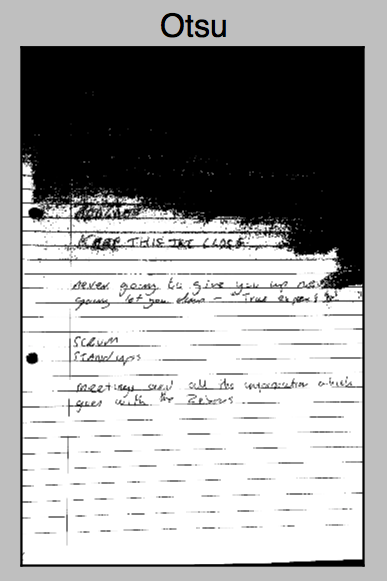
\includegraphics{images/OTSU}
  \caption{The use of Otsu binarisation technique on an image with a shadow across the image}
  \label{fig:OTSU}
\end{figure}

Figure \ref{fig:OTSU} shows the Otsu binarisation method used on an image with a slight shadow over the top right of the image. It can be clearly seen that the binarisation segments the image into two distinct regions: the bottom half is white whereas the top half is black. It can be concluded that this would not be a sufficient solution for identifying characters, when specific regions of the image are unreadable.

Otsu attempts to segment the grey-level values from the image into a series of histograms. Otsu then determines the optimal threshold value by ``maximising the discriminant measure'' \cite{citeulike:2917492}. Essentially, Otsu attempts to maximise the margin between the histograms, this margin would then act as the threshold value as to whether a pixel is segmented into either a foreground or background pixel \cite{citeulike:14021372}.

Hewlett-Packard, the creator of Tesseract, describe Otsu as its underlying pre-processing algorithm when converting the image prior to extracting textlines and characters \cite{citeulike:13931186}. Once the spike work was completed with Otsu, shown in Figure \ref{fig:OTSU}, it was clear to identify that Tesseract would find it difficult to identify the characters from the image when the output was so poorly binarised.

Overall Otsu, although it is a very reliable binarisation method, suffers from imposed shadows over images.

\subsubsection{Adaptive threshold} \label{section:threshold}
As Tesseract uses Otsu as its pre-processing step, using an image which has been binarised with Otsu already would not be advantageous in improving the accuracy of the characters detected. As a result, the next iteration evaluates an adaptive threshold technique.

Adaptive threshold calculates the threshold over a series of smaller segments in the image \cite{citeulike:14021401}. As a result shadows have a smaller impact over the whole image, due to adaptive threshold being a local threshold technique. This makes adaptive thresholding rewarding for non-uniform lighting situations, as it becomes more invariant to shadows.

Using the OpenCV library there was two options with adaptive threshold \cite{citeulike:14021409}:
\begin{enumerate}
  \item Gaussian adaptive threshold: ``the weighted sum of the neighborhood''.
  \item Mean adaptive threshold: ``the mean of the neighborhood''.
\end{enumerate}

\begin{figure}[H]
  \centering
  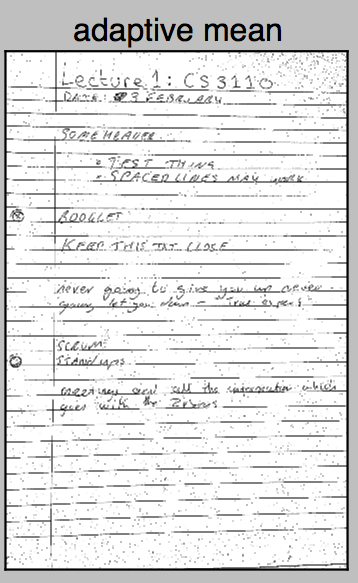
\includegraphics{images/adaptive_mean}
  \caption{Adaptive mean threshold algorithm on a note, showing binarisation but there is still noise in the image.}
  \label{fig:adaptive_mean}
\end{figure}

Mean adaptive threshold uses a specific block size around a given pixel. If the block size was four, then the neighborhood size would be four. It would then calculate the mean pixel value in that block. The mean value is selected as the thresholding value for the pixels inside the block; each of the pixels will then be identified as either foreground or background pixels \cite{citeulike:14021401}. Figure \ref{fig:adaptive_mean} shows mean adaptive threshold being used on an image. An additional issue present with the adaptive mean is the noise pixels as there is considerable amounts of noise polluting the image.

Gaussian adaptive threshold differs from the mean adaptive threshold, as instead of calculating the mean value over the block size, it first uses a Gaussian value over blocksize. A Gaussian weight is calculated dynamically depending on the blocksize used for the thresholding. Each pixel inside the block is then multiplied by the Gaussian, and an average value is then taken across the pixels which is used as a threshold. Like the mean adaptive threshold, this is then used to determine if the pixel is foreground or background \cite{bradski2008learning}\cite{citeulike:14021401}.


\begin{figure}[H]
  \centering
  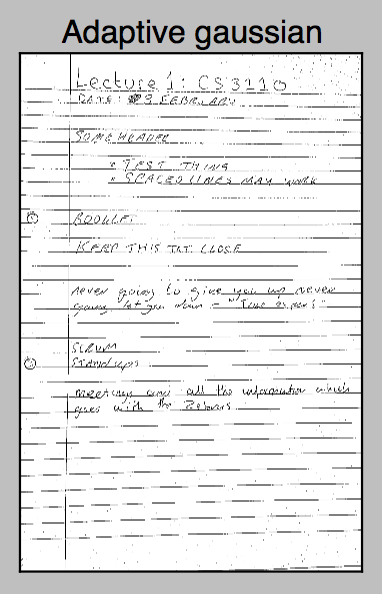
\includegraphics{images/adaptive_gaussian}
  \caption{Adaptive Gaussian used over the image, showing a lot smoother of an image}
  \label{fig:adaptive_gaussian}
\end{figure}

Figure \ref{fig:adaptive_gaussian} shows the adaptive Gaussian being used to binarise an image. The output clearly does not have a shadow overlaying the image and there are fewer noise pixels than the mean adaptive thresholding.

\begin{figure}[H]
  \centering
  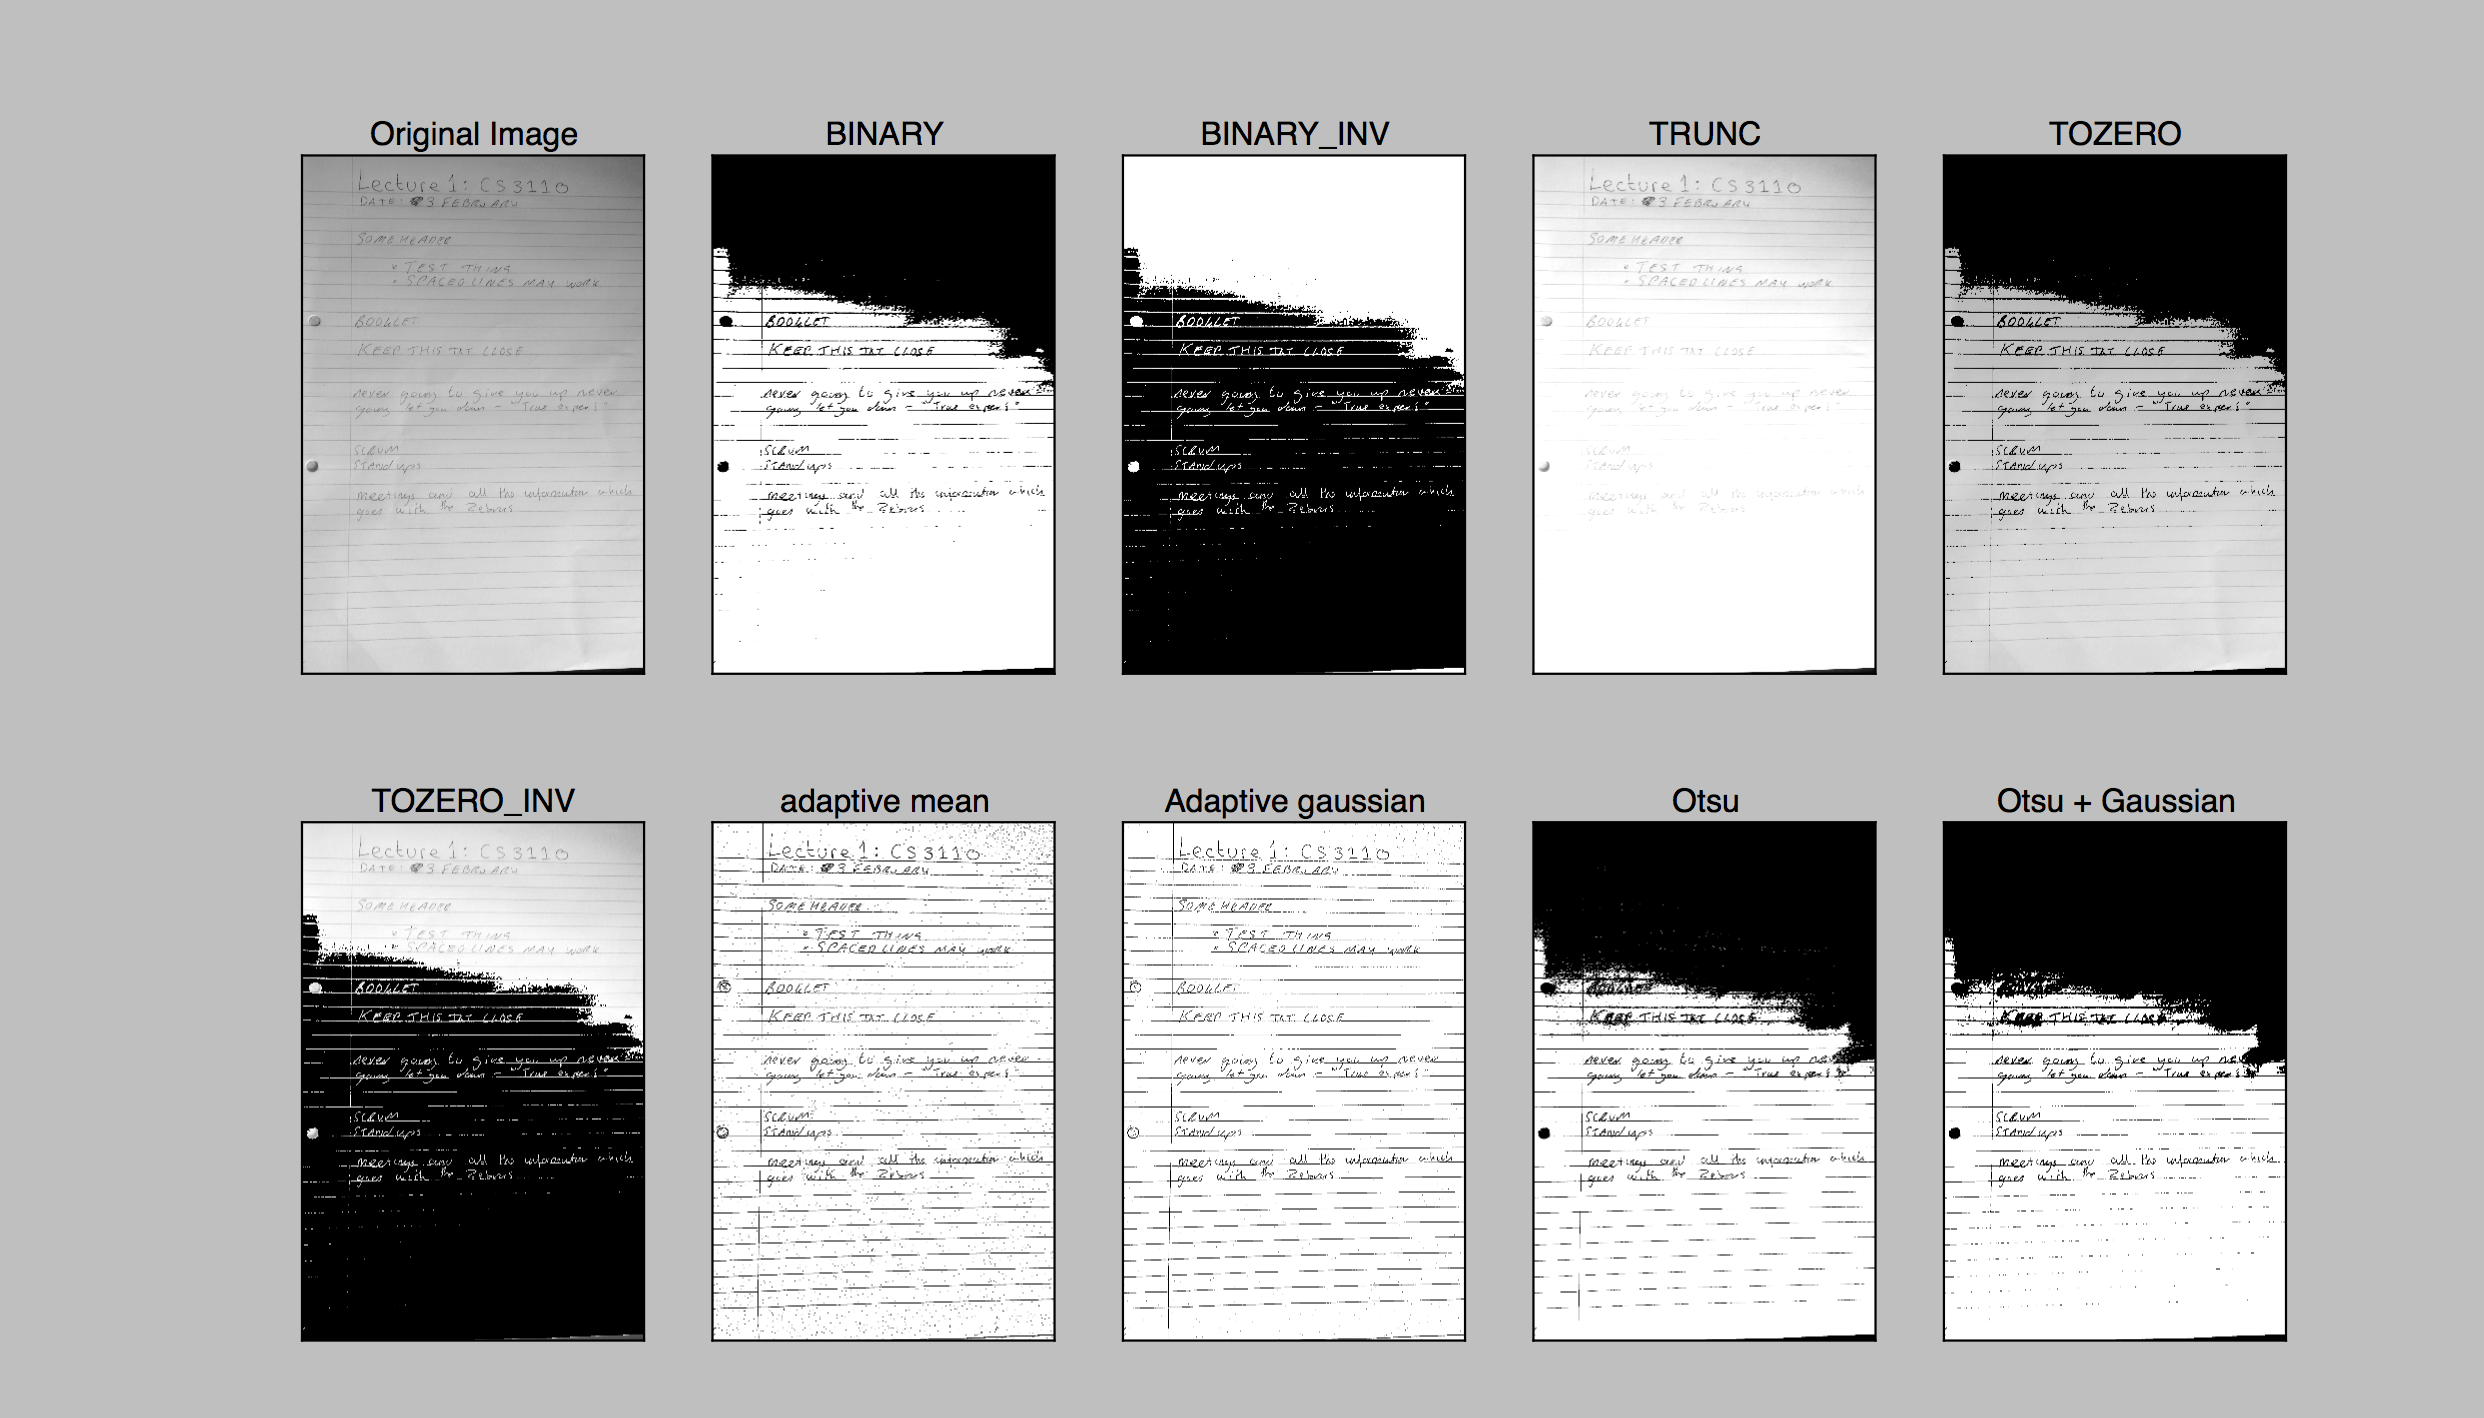
\includegraphics[scale=0.25]{images/thresholding_options}
  \caption{A variety of thresholding techniques used on the same note, showing adaptive threshold resulting in the best output.}
  \label{fig:thresholding_options}
\end{figure}

Figure \ref{fig:thresholding_options} displays additional types of the thresholding that were investigated throughout the iterative process. This example image was adapted from the thresholding tutorial from OpenCV \cite{citeulike:14026982}, and later discarded as it was prototyping work. The Gaussian adaptive threshold provides the clearest results from visual inspection of the different thresholding techniques experimented. As a result, the Gaussian adaptive threshold will be continued to be improved upon throughout a series of iterations to reduce additional noise, via morphological operations to aid in smoothing the image.

\section{Lined paper}
Initially normal lined paper was used for notes in the project, but after the binarisation process it left too much noise. Further smoothing of the image did not remove the noise, so bespoke lined paper was created to aid in removing the lines but keeping the text uniformly straight (refer to Appendix \ref{appendix:image_processing}, Section \ref{fig:pre-line-editing} for more information) .

\subsection{Filtering the blue lines}
Over a series of iterations, the primary objective was to remove the blue lines from the image. Examples of the lined paper can be found in Appendix \ref{appendix:image_processing}.

\begin{algorithm} [H]
\begin{algorithmic}[1]
  \Function{remove\_lines}{}
    \State image $\gets$ read\_image\_as\_grayscale()
    \State lower\_black $\gets$ np.array([0,0,0])
    \State upper\_black $\gets$ np.array([175,20, 95])
    \State mask\_black $\gets$ cv2.inRange(erode, lower\_black, upper\_black)
    \State mask[np.where(mask\_black == 0)] $\gets$ 255
  \EndFunction
  \end{algorithmic}
  \caption{Initial removing the blue lines algorithm}
  \label{algorithm:threshold1}
\end{algorithm}

Algorithm \ref{algorithm:threshold1} attempted to filter all the colour values between a grey and a black range - this was adapted from OpenCV's Changing Colorspaces tutorial \cite{citeulike:14026986}. By restricting it to a specific range it was intended to bypass the blue lines. However, the blue lines would still contain dark pixels - so only segments of the line would be removed.

\begin{figure}[H]
  \centering
  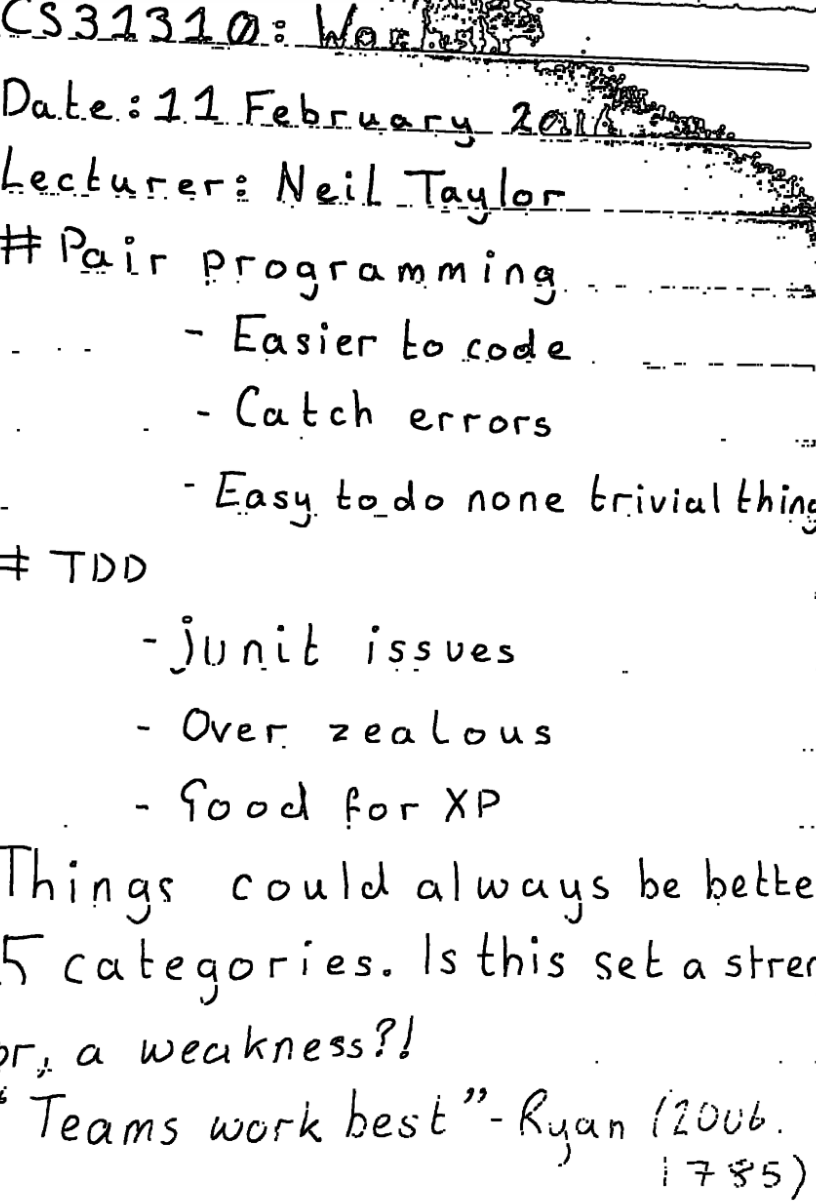
\includegraphics[scale=0.5]{images/removed_lines_still_noise}
  \caption{An example output from the algorithm \ref{algorithm:threshold1}. There are significant amounts of noise in the image.}
  \label{fig:remove_lines_noise}
\end{figure}

Different morphological operations were used on the image in an attempt to clear the noise pixels. Erosion operations were used, by passing a kernel over the image essentially removing small black noise pixels from the white background whilst expanding the darker pixels, enhancing the text on the page \cite{citeulike:14024957}. Dilation is essentially the opposite: a kernel is passed over the image, and the white background areas get larger and the black text gets thinner; this has the effect of removing the characters quality \cite{citeulike:14024957}.

The result of the morphological operations ended up reducing the quality of the segmentation, as shown in Figure \ref{fig:remove_lines_noise}. This highlighted further iterations were needed for an improved output.

\subsection{Only extracting the text}
There was no simplistic way to identify and filter the lines, therefore it was decided that the text would just be extracted.

OpenCV has an example of line extraction and binarsation \cite{citeulike:14006256}. From the example, structuring elements were used to extract the text from the image. Further erosion and dilation were used to remove additional noise. Throughout the process, masks were used to transfer the state of the image to another mask. An example is transferring the text to a mask, but this had an unwanted side effect that line noise way transferred too.

Due to the text having connected pixels, unlike the eroded noise, then connected components were used to identify characters. As a result of  morphological operations the lines were no longer connected. The identified characters were copied to a final mask.

Further smoothing cleared up the image. After a series of iterations the binarisation process was complete.

\begin{figure}[H]
  \centering
  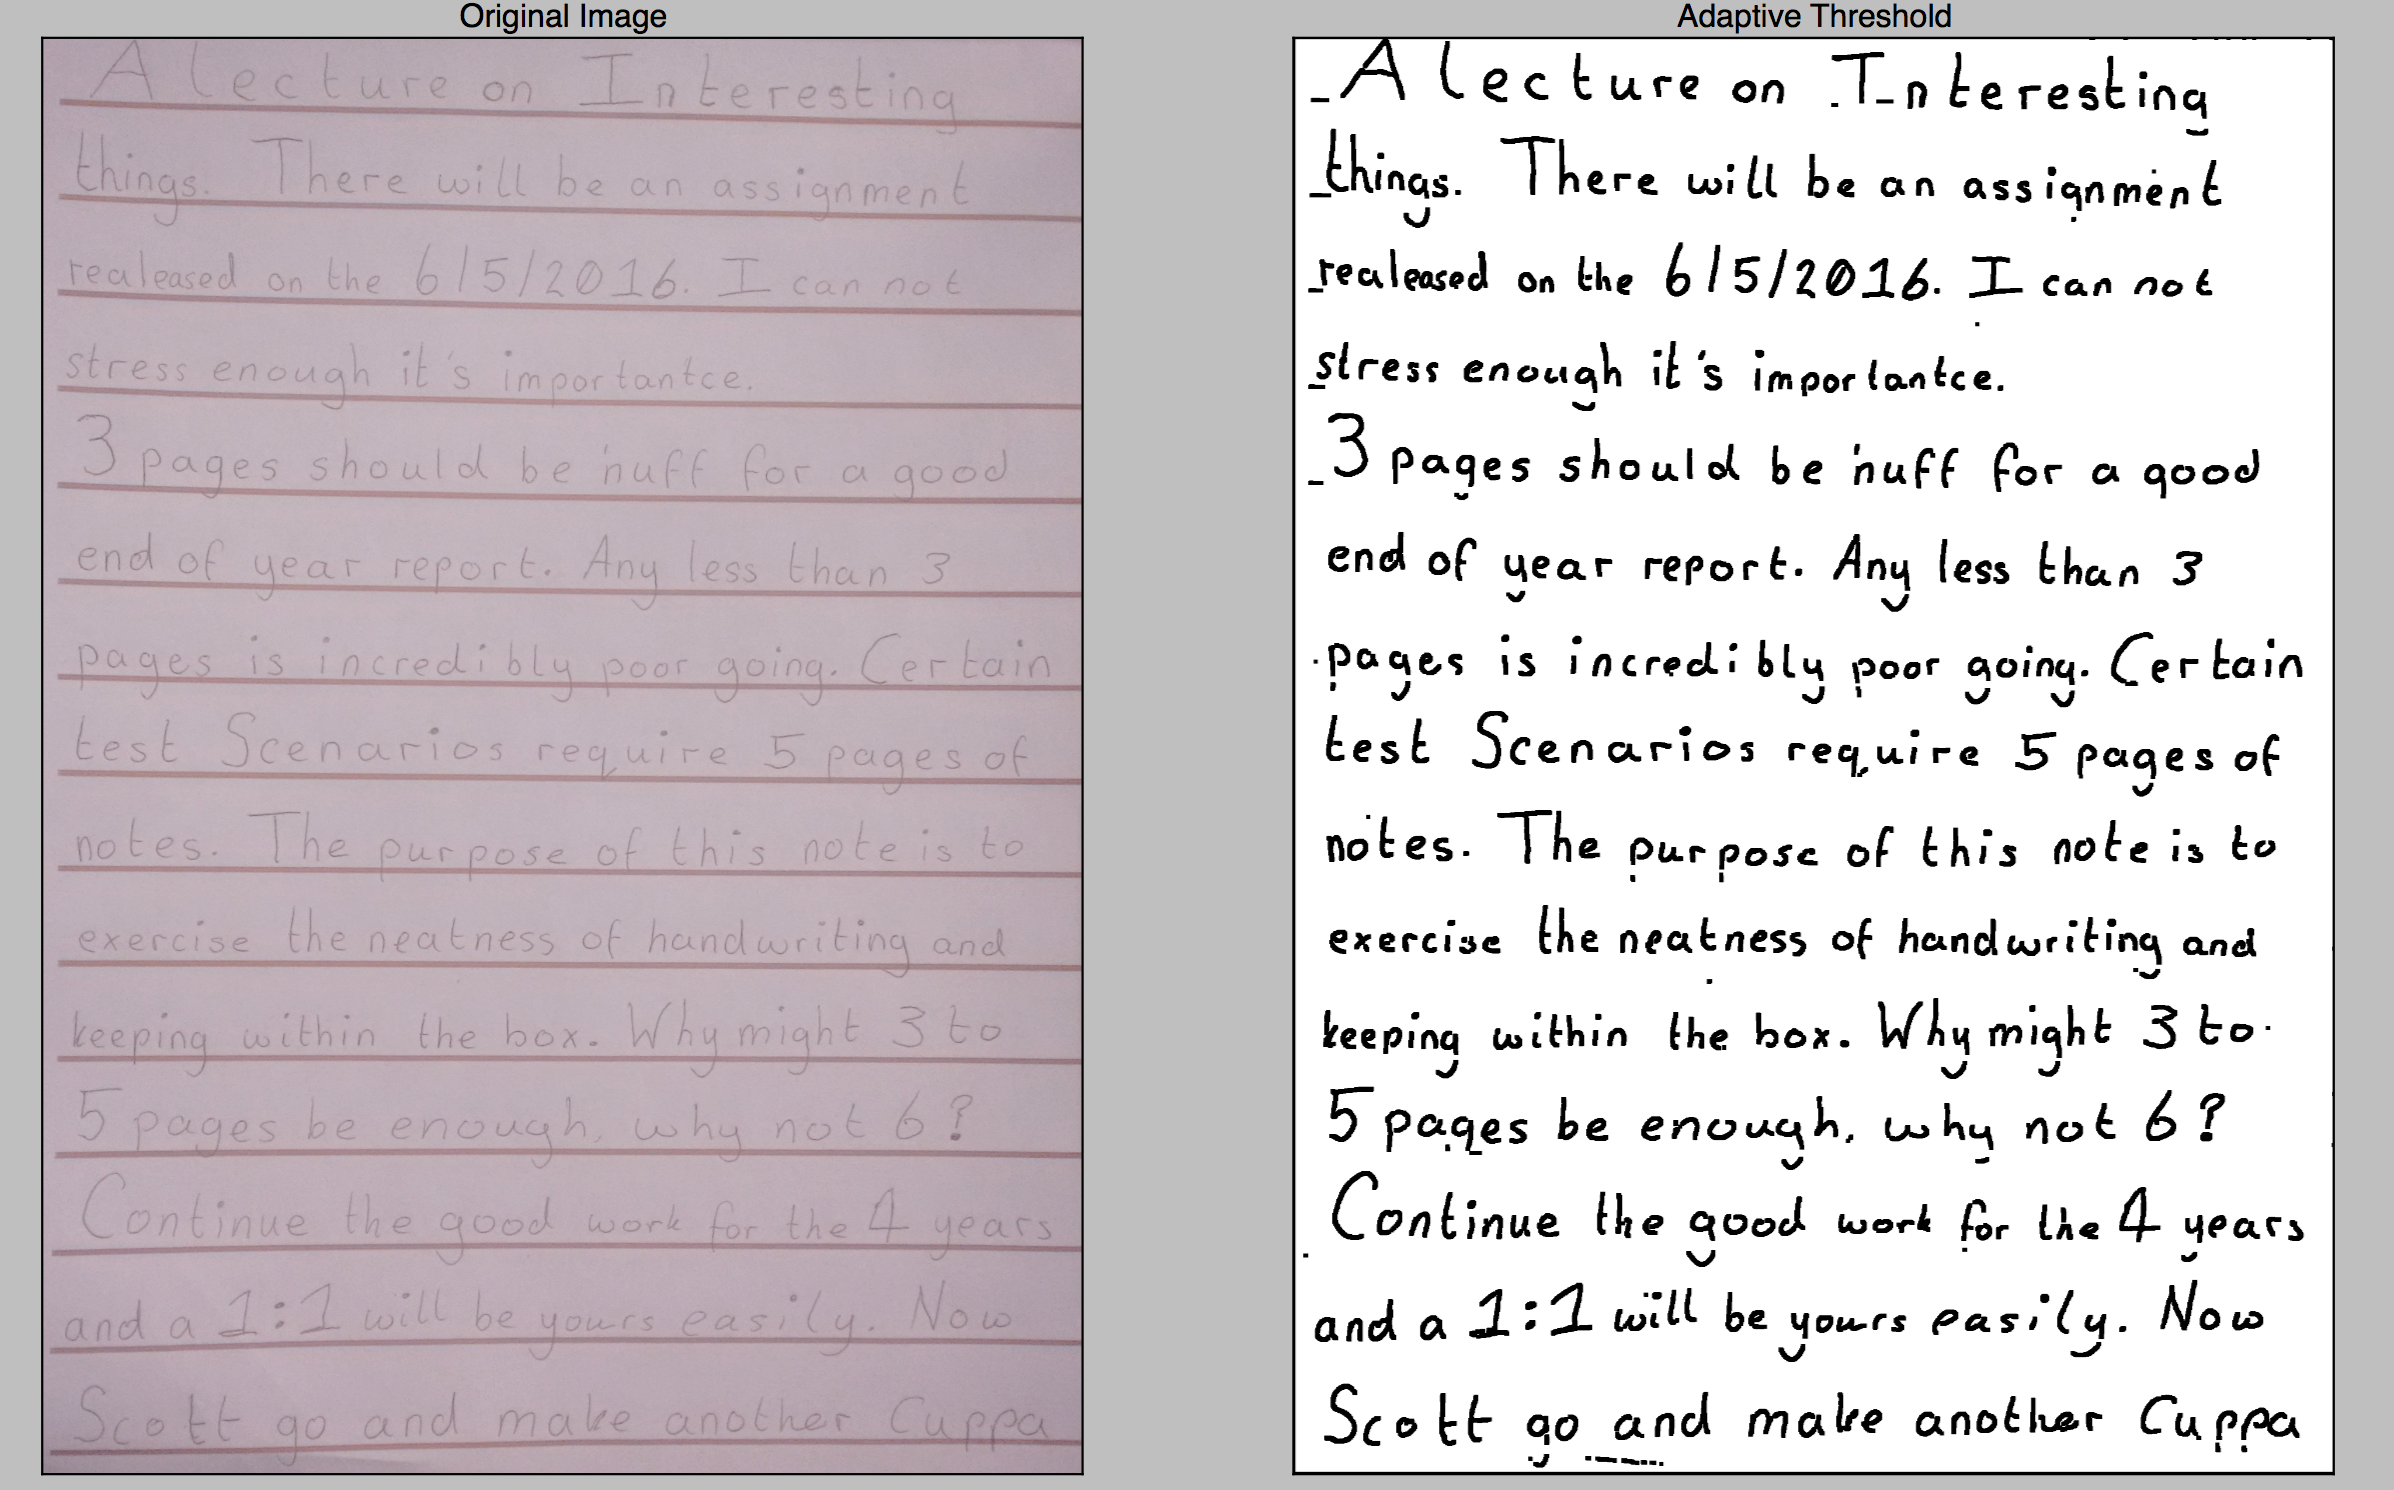
\includegraphics[scale=0.3]{images/hard_image}
  \caption{A poor quality image has been binarised successfully with little noise.}
  \label{fig:poor_quality}
\end{figure}

Figure \ref{fig:poor_quality} shows the result of the binarisation script. Adaptive threshold works well on the image, due to local thresholding not being affected by shadows. Images can be taken in non-uniform lighting and it will produce a fully binarised image. There were issues which affected the implementation such as changing to a bespoke lined paper. Overall the binarisation segmentation works well. Further examples can be found in Appendix \ref{appendix:image_processing}.

\section{Handwriting training}
The training of handwriting was a constant task throughout the sprints. It was initially proving cumbersome in the early sprints. After the changes implemented from Section \ref{section:threshold} the results from the handwriting recognition improved considerably.

\subsection{Training process}
Tesseract's training was a methodical process. Tesseract's GitHub wiki \cite{citeulike:13926796} and Gonzalez \cite{citeulike:13920943}, provided great reference tools on how to train the data.

{{\ttfamily \hyphenchar\the\font=`\-}%
Firstly, as handwriting was being trained a new language would have to be created. Each training example has a specific format which must be adhered to: \texttt{lang.font.expNumber.tiff}. The file is then run through the Tesseract training process using \texttt{batch.nochop makebox} command, on the specific language \texttt{eng.ryan.exp2a}; this created  a box file for the given training example. The box file contains the characters which Tesseract believes are in the image; each line is a new character as shown below:
\begin{center}
  \begin{lstlisting}[basicstyle=\normalsize\ttfamily]
    S 155 2398 208 2487 0
    3 242 2403 295 2485 0
    9 320 2403 376 2476 0
    1 405 2396 448 2467 0
    1 467 2396 504 2462 0
    0 520 2393 588 2455 0
    : 604 2400 628 2451 0
  \end{lstlisting}
\end{center}


{{\ttfamily \hyphenchar\the\font=`\-}%
The box files were too complex to analyse as it was not intuitive to see the identified characters without a graphical interface. Figure \ref{fig:box_editor} shows the use of the jTessBoxEditor \cite{citeulike:13926798} tool to identify characters and their bounding boxes to overcome this issue.

\begin{figure}[H]
  \centering
  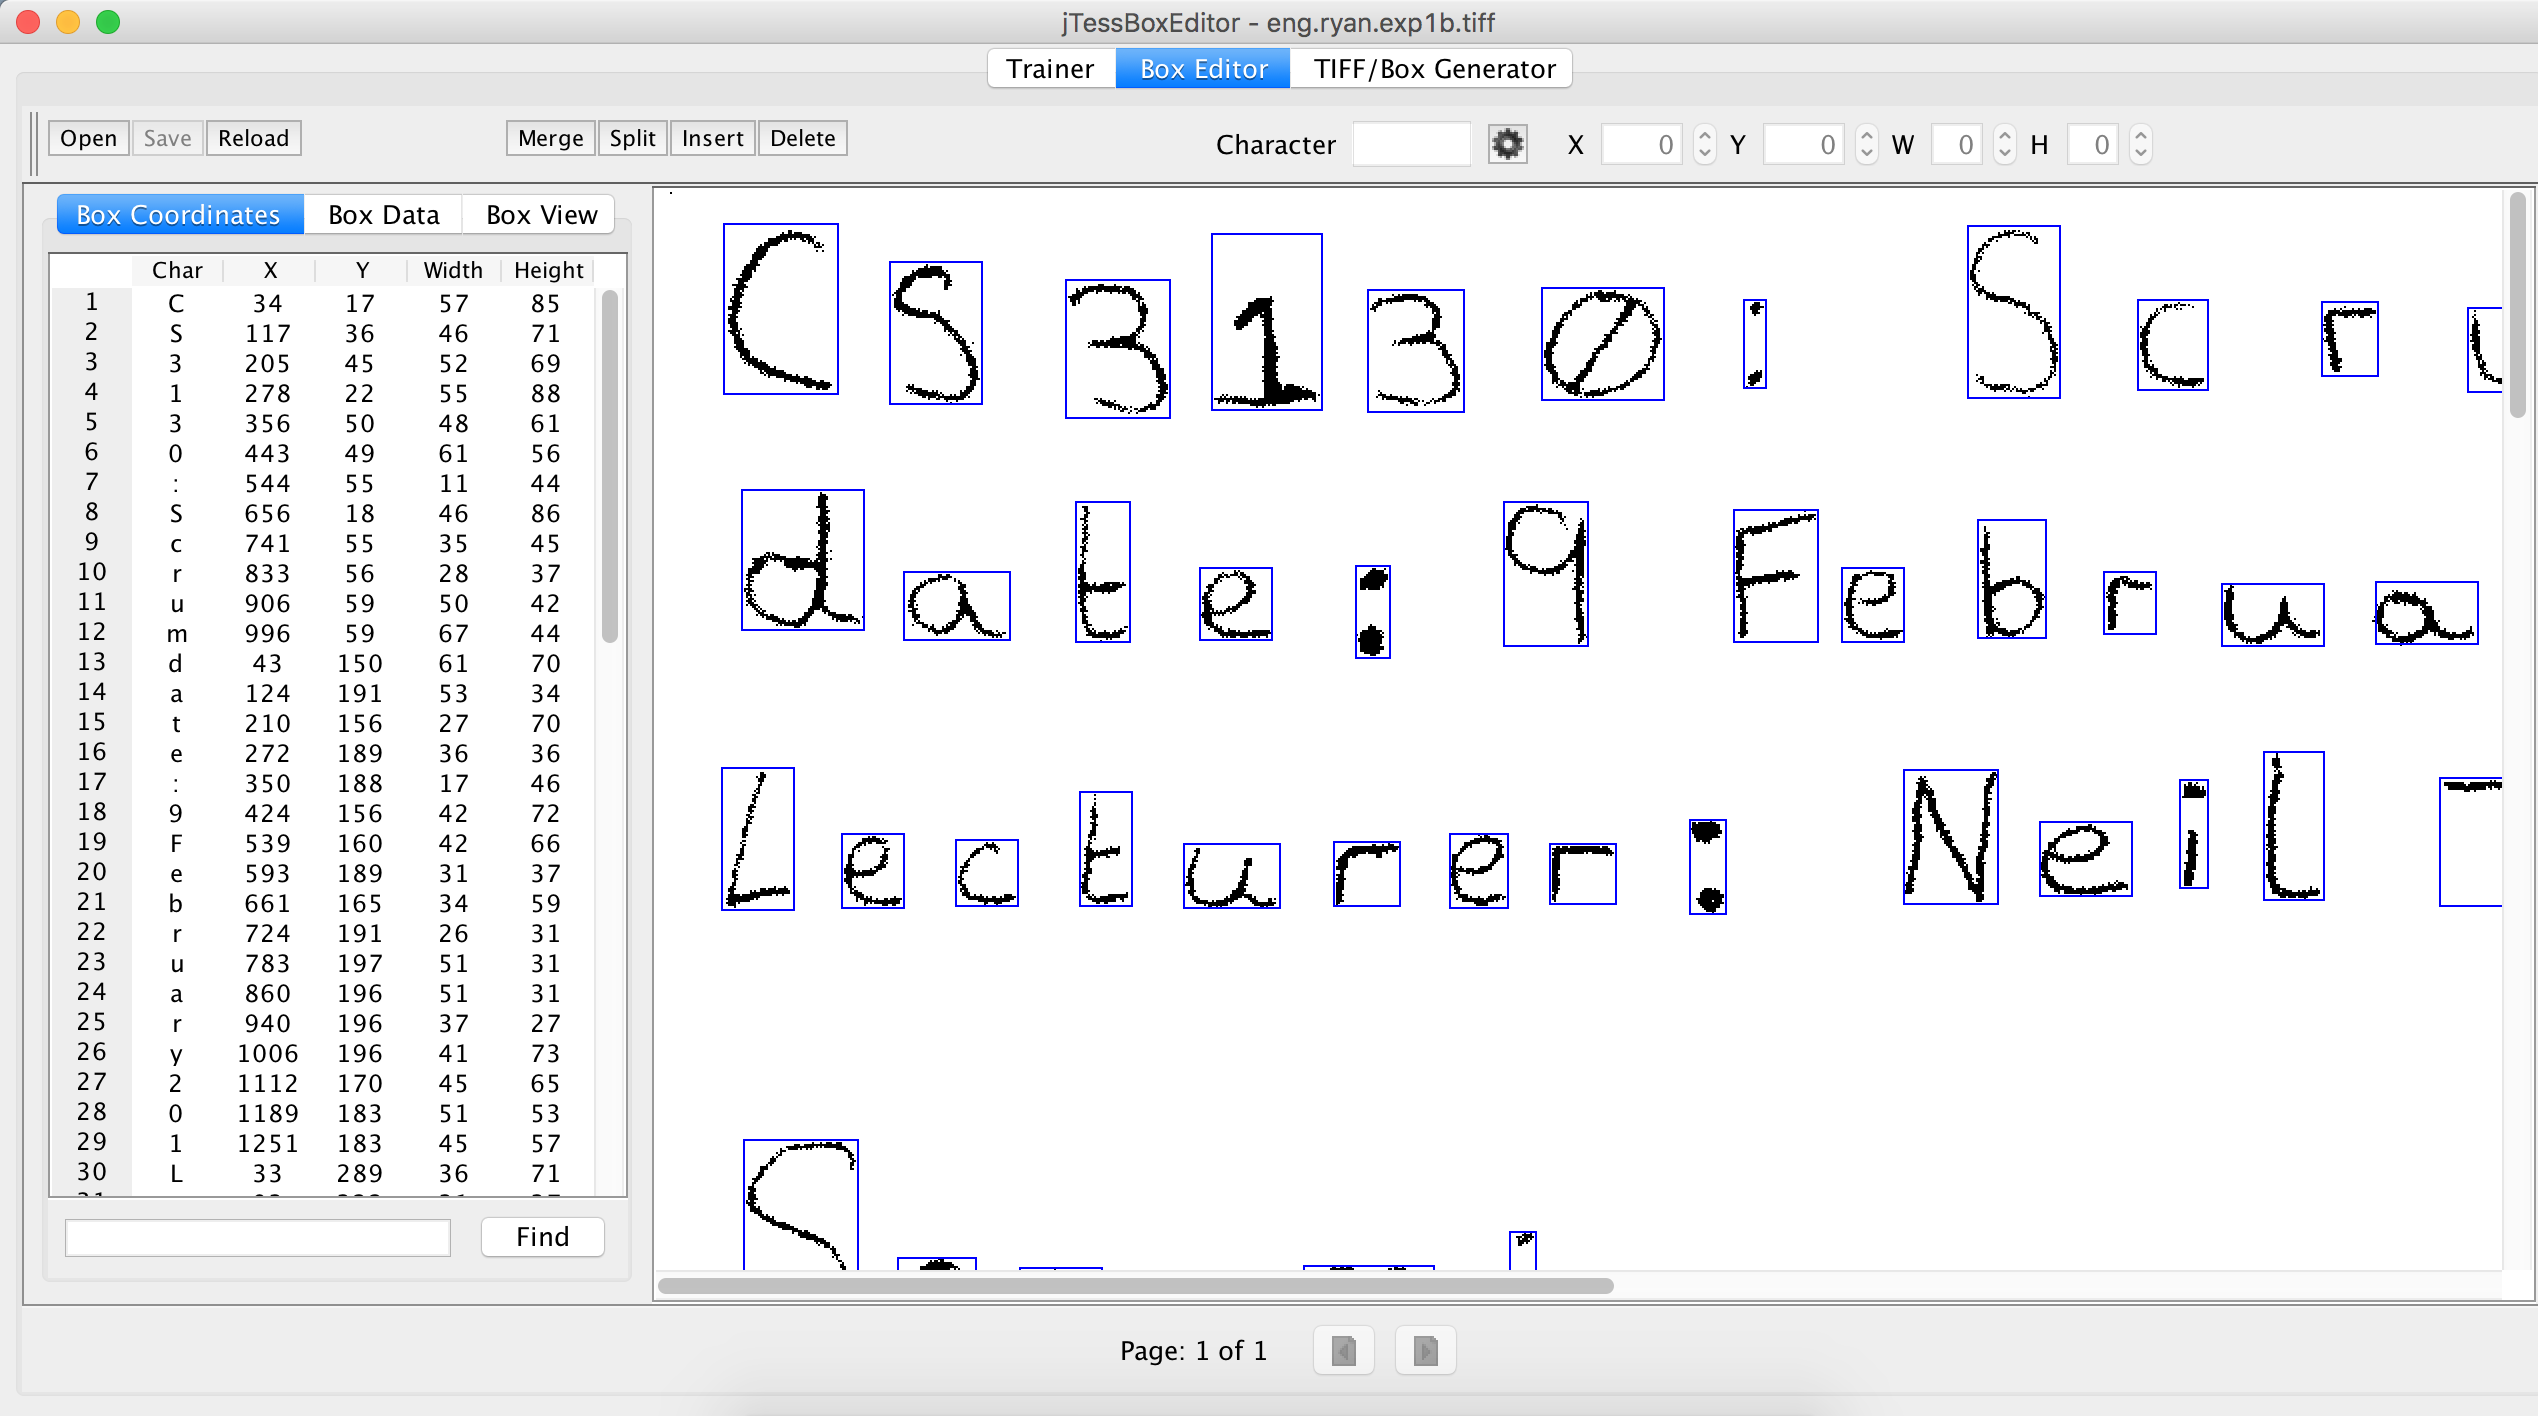
\includegraphics[width=\textwidth]{images/box_editor}
  \caption{A example of the jTessBoxEditor being used identify characters in the tiff box file.}
  \label{fig:box_editor}
\end{figure}

{{\ttfamily \hyphenchar\the\font=`\-}%
Once the characters had been manually changed, the box file was passed through Tesseract's training process. \texttt{tesseract <file> -l eng.ryan.exp2a box.train} would train the engine on the image's box file, for the language \texttt{eng.ryan.exp2a}. Often there were issues with being unable to identify tagged characters; these box file lines were deleted.

{{\ttfamily \hyphenchar\the\font=`\-}%
Following this process, Tesseract required an additional file ( \texttt{unicharset}) to be able to extract all possible characters that were identified in the training examples.

{{\ttfamily \hyphenchar\the\font=`\-}%
Tesseract's GitHub repository states that clustering is an important process to extract `prototypes'. The clustering commands ensured that the shapes of the characters identified are known so they can be used as a reference again.

A frequent words file was created, from the \texttt{/usr/share/dict/words} directory, to help to identify common words. This would aid in improving the chances of detecting specific words. Common words could also be defined; ``by'' and ``date'' are examples of words in this file.

{{\ttfamily \hyphenchar\the\font=`\-}%
Finally, the \texttt{combine\_data} command was used to combine all the data together and output a trained data file in the form of \texttt{eng.ryan.exp2a.trainedddata}. This was then copied to the shared Tesseract data directory enabling new training data to use this language.

{{\ttfamily \hyphenchar\the\font=`\-}%
Reinforcement of the characters identified was needed, so further training examples were created. This was called ``bootstrapping''. Therefore when training on another example, if the language was set to \texttt{eng.ryan.exp2a} it would reinforce that specific language with new data.

Throughout the sprints issues were identified whilst training the data. Characters would often not be identified correctly on the image, with specific issues with the letter ``g''  identified as the number 3. When a blob could not be identified at all, Tesseract would label it ``$\thicksim $''; these were ultimately removed when it was discovered that it would fail to identify them if edited. The training was conducted on twelve training examples, a selection can be found in Appendix \ref{tesseract:training}.

\section{Web application}
The web application was the main part of the development and specific sections proved to be more complex than anticipated.

\subsection{OAuth}\label{app:oauth}
The Google OAuth integration was more complex than first considered. Google suggested to use the Google client library \cite{citeulike:14024993} for all OAuth requests, to avoid security issues when making requests. Therefore, this library was utilised throughout the project.

The Google API client would, on occasion, raise peculiar errors. Whilst making a query to the calendar API it would raise the error, `rootURL', when using the build API call. This was mystifying as it was previously working. An issue was raised on the library's GitHub repository \cite{citeulike:14021433}. To confuse matters more, when querying the Google people plus API, it would work perfectly fine - however the Google Calendar API would raise an exception. It eventually stopped raising an exception, but the reason is unknown.

OAuth2 was implemented in the application so when the user clicks `authorise with Google' it will initialise the process for OAuth.
Once the user accepts the use of selected services a secure JSON \footnote{JavaScript Object notation is stored in key-value pairs.} credential file was returned containing specific tokens used when querying; these are appended to the user's session.

The credentials contain an expiration time, as shown in Appendix \ref{oauth:response}. When making a request this expiration time was checked, and if it was exceeded, then an error would be raised when querying the API's and displayed to the user. To overcome this, additional checks were made to ensure the credentials in the session were still valid. If they were not then it would redirect the user to the log-out route, clearing the session and asking the user to re-authenticate.

\subsection{Reoccurring events}
Reoccurring events within the Google Calendar integration posed a lot of issues. It was identified in the pre-beta testing that if the user has a reoccurring event then it would not append the URL of the note to the event.

When a query was made for a list of events, if there were reoccurring events then it would group the events by the first instance of these events. This proved to be problematic as it would display to the user that the note was taken on the 12th March, for example, but there were events from February being shown.

To account for this, the structure of the response was analysed and it was identified that grouped events had a \texttt{reoccurrenceID} key. After finding that the calendar API can fetch reoccurring items, a query was made using this ID key - filtering by the start and end date from the initial query. A check was included to ensure that when displaying to the user the event did not contain the \texttt{reoccurrenceID} key ensuring the singular events were displayed to the user.

Editing a reoccurring event produced further unexpected behaviour: when the event had been successfully modified and the note URL had been appended, it returned both the grouped event and the modified edited event in the initial query. Google must determine that changed reoccurring events are new instances. Instead of displaying more duplicated events to the user, a check for the \texttt{recurringEventId} key, which was present in the modified event, was conducted; if it was present the event was omitted.

Another issue identified were all-day events. All-day events do not have a datetime key in their start response field, returned from the Google Calendar API. This would cause the application to raise an exception and prevent the user from adding a note. A check was made to make sure that the datetime key was present.

\subsection{Tesseract confidence}
Displaying the Tesseract data went through a series of iterations over the latter sprints.

At a basic level, integrating Tesseract into the web application was fairly simple and was implemented at around sprint eight. The binarisation script (see Section \ref{imp:image_proces}), was incorporated into the application. This was added to the file upload route, as the user's image needs to be binarised when it is uploaded. A Tesseract wrapper could have been implemented but due to time constraints a third party library, tesserocr \cite{citeulike:14021437}, was used.

\begin{figure}[H]
  \centering
  
\includegraphics[scale=0.7]{images/tesseract_first}
  \label{fig:tesseract_output}
  \caption{Tesseract being integrated into the application at a very basic level}
\end{figure}

Tesserocr is a Python wrapper for Tesseract's  C++ API. Tesserocr uses textlines to extract the text from the uploaded image. The first three lines were then iterated over, identifying the box for the lines so that text could be extracted. Each of these lines mapped the words identified and the confidence score for each word on a scale of 0 - 100 (0 being uncertain and 100 being certain).

The module code, lecturer, location and date were extracted via list-comprehensions, matching the metadata structure defined in Section \ref{design:tesseract}. Modifications to the confidence scores were attempted in the controller to replace with a class name for the colours - so that the view file could render the content easily. Problems were encountered when the API returned tuples, an immutable type, so modifications were not as eloquent as originally envisaged, therefore numbers remained.

Conditional checks were made in the view files on the confidence score; 75 would be green text, less than 74 and greater than 70 would be orange text and below 65 would be red text. Figure \ref{fig:tesseract_colour} shows the resulting output from the conditional checks. There are anomalies, with ``Date'' for example, it is orange but in fact it is extracted perfectly.
\begin{figure}[H]
  \centering
  \begin{subfigure}[h]{0.35\textwidth}
    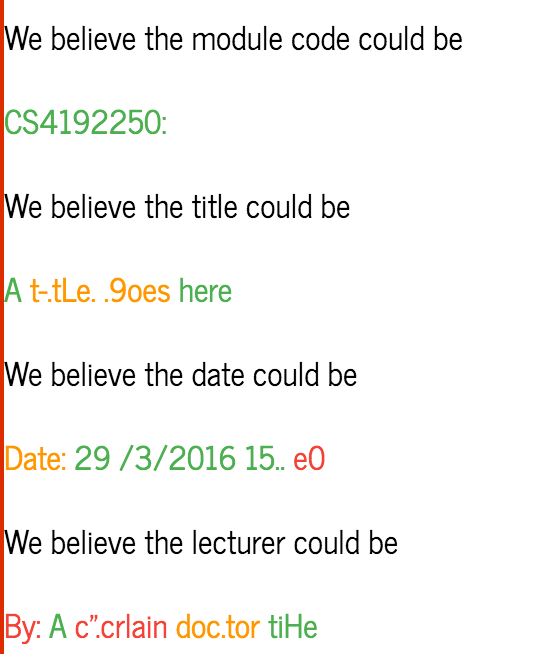
\includegraphics[scale=0.35]{images/tesseract_colour}
    \caption{}
    \label{fig:first_tesseract}
  \end{subfigure}
  \hspace{1em}
  \begin{subfigure}[h]{0.35\textwidth}
    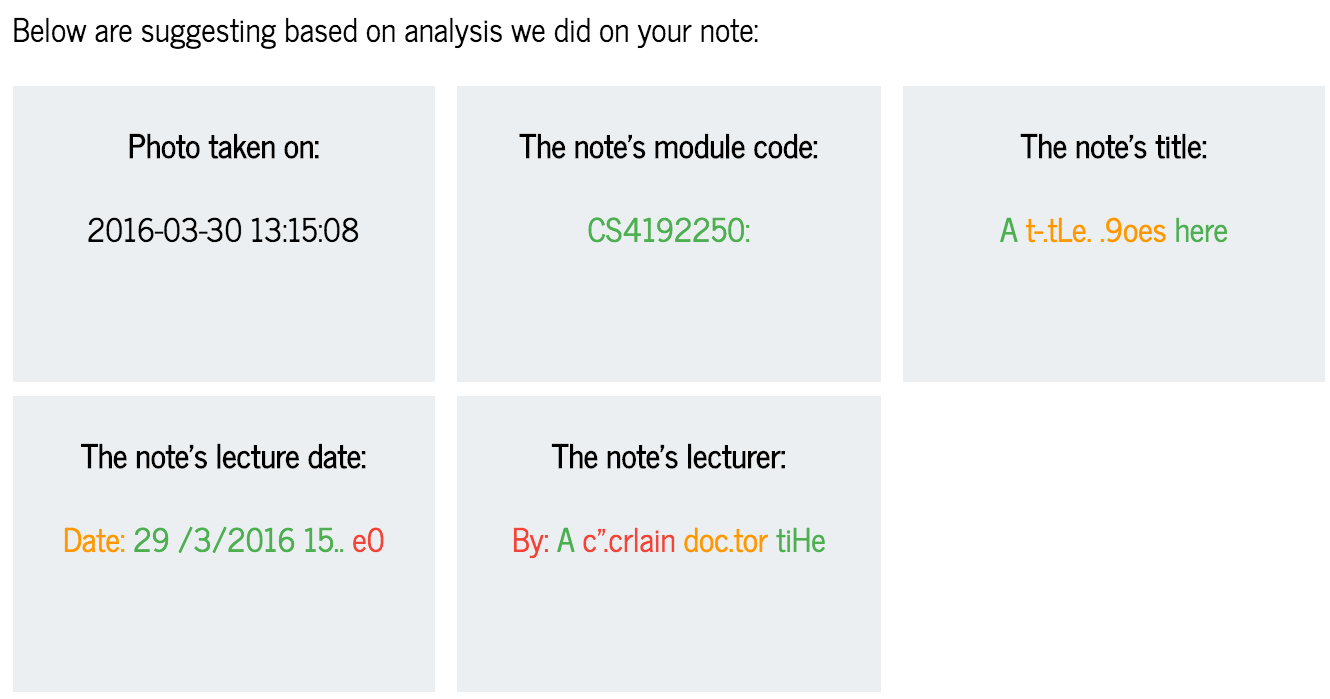
\includegraphics[scale=0.3]{images/styled-tesseract-data}
    \caption{}
    \label{fig:second_tesseract}
  \end{subfigure}
  \caption{Coloured representation of the confidence of the words from the handwriting: a) shows the initial steps with the image. b) shows the resulting output after styling of the web application}
  \label{fig:tesseract_colour}

\end{figure}

\subsection{Parsing EXIF data}
EXIF data parsing would be an important section of the application. EXIF data is essentially metadata about an image \cite{citeulike:14024991}. When a user uploads a note, it analyses the image for the EXIF metadata; it  uses the date of the image taken to query Google Calendar for additional events.

Throughout the sprints the EXIF data parsing was extended to allow for a greater variation in images uploaded. Python's image library \cite{citeulike:14024992} was used to parse the data. Further additional checks were made to ensure that the images were either JPEG or TIFF as they only contain the metadata.

During user testing, issues arose where a participant could not upload their note successfully. The image was formatted a JPEG but the mobile phone photo did not contain the `dateTime' EXIF key. Checks were implemented to ensure that this key existed.

\subsection{Displaying calendar events}
Over several user stories, events were displayed throughout the application. The first instance of this was displaying the events from the last seven days, from the user's calendar, on the homepage - shown in Figure \ref{fig:seven_days}. This was simple to implement but provided a strong foothold into the interactions with the Google Calendar API; this stretched from the application to the testing infrastructure.

\begin{figure}[H]
  \centering
  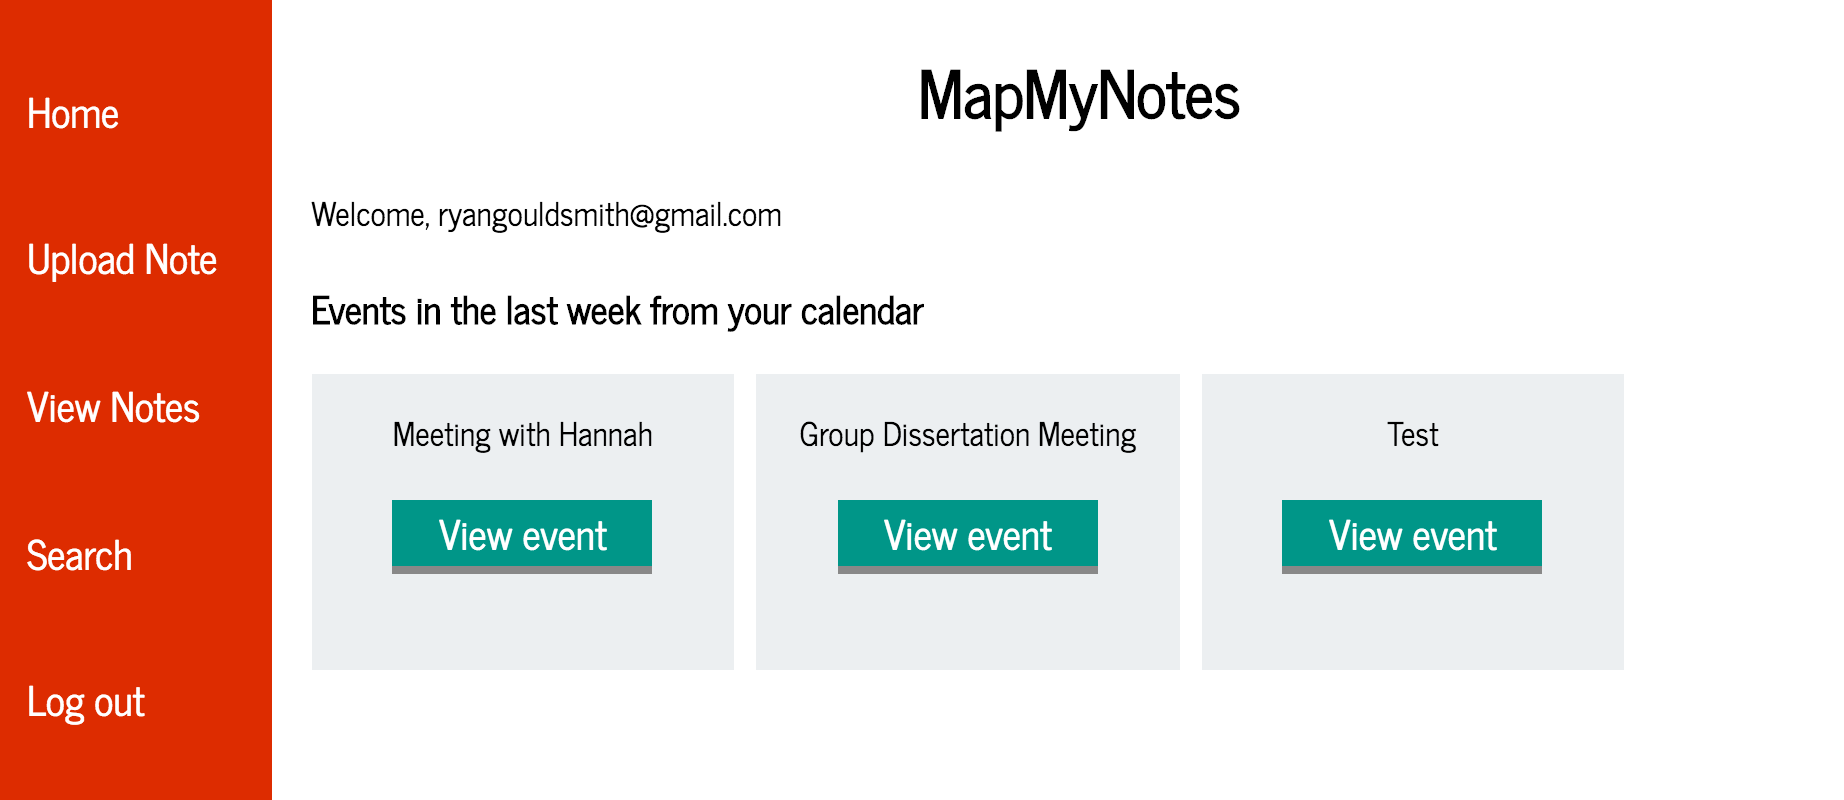
\includegraphics[scale=0.5]{images/event_seven_day}
  \caption{An example of displaying the events from the last week from the user's calendar}
  \label{fig:seven_days}
\end{figure}

One issue which arose was the change in timezones to British Summer Time during the project. If there was an event starting at 14:00, and the user queried for events at 14:00, then it would not return any results from the Google Calendar. Upon closer inspection if the query was for 13:00 then it would return the correct event. This issue rendered the application to a halt whilst this could be fixed: eventually, the timezone was appended to the user's input and querying with the timezone included returned the correct event from Google.

\subsection{Editing calendar events}
The user story for adding a note was implemented, and as part of the tasks for this story the note URL must be saved in the calendar event. When the user enters the date into the form, a query would be made to the Google Calendar API to return all associated events from that given day. Checks were then performed to ensure that the module code and the summary of the event matched.

This posed the problem of being able to add the note's URL to the correct event; if there was more than one event with the same module code that day then there could be confusion as to which event to add to.
Over the next iteration of development, the calendar events were additionally validated against the start date from the event and the user's input.

One issue which arose when adding the note's URL to the description field of the calendar was that it would replace the original content inside the description. This is a major concern for the users of the application as it would overwrite any data. Another issue it created was that multiple notes could not be attached to a given event. This was changed so that it would append to the description field, rather than overwriting it.

The algorithm for adding to a calendar is stated below.
\begin{algorithm}
  \caption{Adding a note URL to the calendar}
  \label{algorithm:threshold2}
  \begin{algorithmic}[1]
      \State Create a calendar service object
      \State Prepare URL from saved note
      \State Build the HTTP request
      \State Find an event for that day from the start time as given
      \State Parse the events
      \State Check to see if the summary contains module code AND the start date time matches
      \If{contains module code}
        \State check the response to see if description includes URL
        \State Save URL to the notes attribute in the database
      \EndIf
  \end{algorithmic}
\end{algorithm}

\begin{figure}[H]
  \centering
  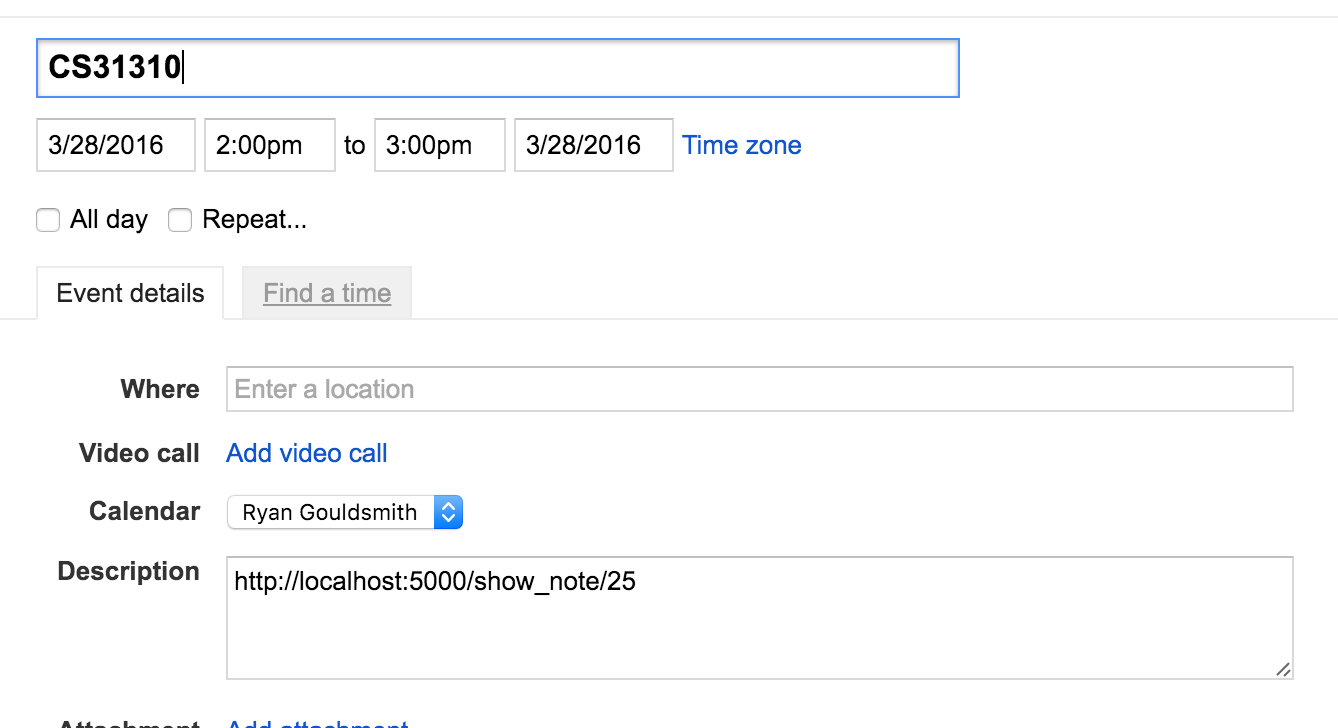
\includegraphics[scale=0.5]{images/saved_to_calendar}
  \caption{Saving a note correctly to a calendar event item}
  \label{fig:saved_to_calendar}
\end{figure}

Figure \ref{fig:saved_to_calendar} shows the output from saving a note to a specific date and appending the note's URL to the description field.

\subsubsection{Editing a note}
The user story ``editing a note'' was established midway through the project. An example task included when editing a note's start date it should be reflected in the user's calendar. If the user changes their date then it should remove the URL from the old calendar item and append to a new one, if the event exists. This proved to be a complicated implementation.

When a user edits a note it would query the API to return the event for the given note, based on the time start which was persisted for the note's relation. This event was then modified by replacing the description field with an empty string, replacing all the content. This caused issues regarding the data stored by the user being deleted arbitrarily. As a result a find and replace was used on the description field to remove any strings which matched the URL.

It is worth acknowledging at this point in the development considerable aspects of the codebase was refactored. There was duplicated functionality spread across multiple blueprints, making the codebase obfuscated. As a result the design decision for the \texttt{GoogleServicesHelper} emerged to abstract the duplication.

\subsubsection{Logging in and out}
Enabling the system to have users was an emerging user story midway through the project. As the log in would be deferred to Google, then the user would need to connect to the service. When the log in process has been completed, a user's email address is extracted from the Google Plus API response and created in the database.

Using the application it was noticed that multiple users were being created for a single email address. To reduce this problem a helper function was implemented which would find a user from their email address, if the user could not be found then they were added to the relation.

The user's ID is then appended to the session. Every page on the application verifies that this key exists. Once a user had finished using the application, the log-out route would destroy the user's session.

Delegating the responsibility to Google was a good design decision; the security which Google has would have been better than what could be implemented by the author. Furthermore, ethically, the only personal information the system uses from a user is their email address.

\subsection{Saving and editing a note}
Prior to saving a note the associated relations had to be created. The aim was to use migration files, which would help to keep versions of the different stages which the relation was developed. Flask did not implement migrations by default, so Flask-Migrate \cite{citeulike:14025941} was used as it is an extension to create migration files. Migration files are run when a change was needed to be made to a relation, this was performed through Flask-Script \cite{citeulike:14025943}. An excerpt is shown below:

\begin{lstlisting}[language=python, caption={An excerpt of a specific migration file where the note relation was created}, label={migration}, breaklines, columns=fullflexible, keywordstyle=\color{blue}, basicstyle=\normalsize\ttfamily]
  def upgrade():
    op.create_table(
          'notes',
          sa.Column('id', sa.Integer, primary_key = True),
          sa.Column('image_path', sa.String(150), nullable=False)
    )
  def downgrade():
    op.drop_table('notes')
\end{lstlisting}

The listing \ref{migration} the \texttt{upgrade} function would be run when the migration is performed. As shown the revisions were developed iteratively, depending on the functionality being implemented.

The route \texttt{add\_meta\_data} was created allowing for a HTTP POST request to be made. The controller checked for the associated key values from the request object. Before the parameters were forwarded onto the models checks were conducted to see if the module code already existed. Using the Flask-SQLAlchemy \cite{citeulike:14025864} API's it was simple to extract the module code using the \texttt{like} API.



Flask-SQLAlchemy interacts with relational databases and enabled an Object-Relational Mapping (ORM) style syntax. Relationships could be constructed between the different relations. Listing \ref{orm_syntax} shows an example of how a query can be created, such that it is structurally identical to an object oriented design.

\begin{lstlisting}[language=python, caption={The module code class calls the module code attribute and compared its value against a prepared module code.}, label={orm_syntax}, breaklines, columns=fullflexible, keywordstyle=\color{blue}, basicstyle=\normalsize\ttfamily]
    query = ModuleCode.module_code.like(prepared_module_code)
\end{lstlisting}

A similar principle was adopted for the finding existing metadata items from the relation. The extraction of similar metadata items just compared the different attributes which make up a relation, which were then returned.

If the edit data query returned any results then this ID was used for the notes foreign key to the \texttt{NoteMetaData} relation. If there were no results returned the data was created in the constructor for a new instance of the relation.

The code was becoming obfuscated with database session handling, so a \texttt{save} function was created to abstract this code. Listings \ref{save_function} displays persisting an instance to the relation.
\begin{lstlisting}[language=python, caption={Save function that was abstracted to remove the db session handling from the controller}, label={save_function}, breaklines, columns=fullflexible, keywordstyle=\color{blue}, basicstyle=\normalsize\ttfamily]
  def save(self):
    db.session.add(self)
    db.session.commit()
\end{lstlisting}

{{\ttfamily \hyphenchar\the\font=`\-}%
Editing a note is very much the same except the data is sent via an HTTP post to

\noindent
\texttt{/edit\_meta\_data/:id} where the ID is the note's ID which is currently being edited.

\section{Travis}
Although not strictly a coding implementation, Travis formed a core part of the application and issues were found whilst using Travis.

Firstly, at the start of the process extensive time was invested into trying to  auto-deploy from Travis. Whilst giving detailed instructions on how to deploy to third party systems the documentation for deployment to a virtual private server was sparse. Over several sprints the auto-deploy pipeline was desired but due to the lack of documentation there was no auto-deployment from Travis to a server.

When integrating Tesseract with the application, it became apparent of an issue with Travis: Tesseract and OpenCV had to be both built from source. TesserOCR uses Tesseract 3.04, and at the time of writing, Ubuntu's latest package is 3.02; this is the same for OpenCV 3.0.0. As a result, the build time for Travis was increased exponentially. The current build time was around thirty minutes; caching was investigated but no suitable solution was identified.

\chapter{Testing}

Detailed descriptions of every test case are definitely not what is required here. What is important is to show that you adopted a sensible strategy that was, in principle, capable of testing the system adequately even if you did not have the time to test the system fully.

Have you tested your system on �real users�? For example, if your system is supposed to solve a problem for a business, then it would be appropriate to present your approach to involve the users in the testing process and to record the results that you obtained. Depending on the level of detail, it is likely that you would put any detailed results in an appendix.

The following sections indicate some areas you might include. Other sections may be more appropriate to your project. 

\section{Overall Approach to Testing}

\section{Automated Testing}

\subsection{Unit Tests}

\subsection{User Interface Testing}

\subsection{Stress Testing}

\subsection{Other types of testing}

\section{Integration Testing}

\section{User Testing}
\chapter{Evaluation}

%Examiners expect to find in your dissertation a section addressing such questions as:

%\begin{itemize}
%   \item Were the requirements correctly identified?
%   \item Were the design decisions correct?
%   \item Could a more suitable set of tools have been chosen?
%   \item How well did the software meet the needs of those who were expecting to use it?
%   \item How well were any other project aims achieved?
%   \item If you were starting again, what would you do differently?
%\end{itemize}

%Such material is regarded as an important part of the dissertation; it should demonstrate that you are capable not only of carrying out a piece of work but also of thinking critically about how you did it and how you might have done it better. This is seen as an important part of an honours degree.

%There will be good things and room for improvement with any project. As you write this section, identify and discuss the parts of the work that went well and also consider ways in which the work could be improved.

%Review the discussion on the Evaluation section from the lectures. A recording is available on Blackboard.

\section{Correctly identified requirements}
To recap, the following requirements and objectives were identified at the beginning of the project:
\begin{enumerate}
	\item Investigate how to extract handwriting text from an image - this will involve looking into ways OCR tools can interpret handwriting.
	\item Train the OCR to recognise text of the author's handwriting.
	\item Produce a set of a rules which a note must comply to.
	\item Produce a web application to form the core part of the product. This includes allowing a user to upload an image, display the image. Add appropriate tagging to a note such as module code.
	\item The user must be able to search for a given module code, showing the fill list of notes based on the module code entered.
	\item The backend of the application must conduct basic OCR recognition, analysing the first 3 lines of the notes.
	\item The backend must integrate with a calendar to archive the notes away later to be found again.
\end{enumerate}

The afformentioned requirements were part of the core system requirements; these were classufied as the minimum which the application must do. Personally, these targets, partly self-imposed, were extremeley challenging. The amount of work that was taken on, with lots of different components required that work was produced at a steady pace.

Investigation and research work was extensively conducted to identify how handwriting can be extract from an image. This was further enhanced by looking to optimise the performance of the Tesseract engine. Not only was the image binarised - there were studies and iterations of improvemet which would help to benefit the end user.

After twelve different training examples, from hand, the Tesseract enging is not yielding any greater of a success. Therefore it can be concluded that a sufficient job has been achieved with handwriting training. Probably one of the most frustrating experiences with labelling individual characters. Nevertheless, the training could not return a greater success than currently therefore good work has been completed to get it to that stage.

With the web application being the core part of the problem, then a lot of effort was centered in on ensuring the correct functionality was added. Personally, the application reflects that of the work carried out on it. A user can upload an image to the application and tag all associated meta-data, including the title, module code, date, and location.

The application creates an easy to use interface that allows the user to search for a given module code with ease. The case in which they enter the text is not important, as the application handles the case-sensitivity allowing for a better user experience.

One of the more impressing features of the application is the handwriting recognition integration. It parses the first three lines of the image and shows it to the user in an intuititve manner. This was built ontop of the work already implemented in the project with the handwriting recognition. With the final steps included the application has its true purpose, and that extra bit of complexity which personally the application needed.

Finally, from the original requirements the calendar integration was succesfully implemented; it was in retrospect one of the more challenging tasks to overcome. Ranging from the testing the services to implementing reocurring events, Google calendar always threw up a lot of issues. The reocurring events and all day events were particially frustrating, however there has been a wide interaction with the calendar. It can list all events in the last 7 days, find specific events by day and is able to find reocurring events. Ontop of this is can add to an event description and remove a specific string from the description field.

Overall, the application produced meets all the core requirements and goes beyond, in some aspects, the original features. The app has been well tested with a strong testing infrastructure backing the application. There have been complex design decisions to ensure that the design of the application is simple and intuitive to a reader. Personally, the app has been completed to a good standard.

\section{Design decisions}
Reflecting on the design decisions which were evaluated in section x. The use of the MVC framework structure was extremely beneficial. It encouraged that the code was decoupled at all times, leaving the system extremely modular. Spending the time to construct a good MVC structure was worth it.

The overall database diagram is well considered, and each of the relations is correctly identified and considered. One aspect which would be nice to change would be the note relation, so that the image path was represented in its own relation.

Additionally, there are a few functions in the binarise image class which should be static.

Overall, the design of the classes show a good level of understanding regarding the object oriented paradigm. The use of helpers and service objects help to extend the system, reducing the amount of duplicated code, whilst semantically collating similarily related code together.

Although not strictly related to the core design of the system, but it was wished that the PEP8 [CITE] standard was followed and implemented as the application was being developed. Due to inexperiences using Python, this was not realised until later on in the project - this resulted in a larger refactor and reflecting it should have been conducted at the very beginning.

\section{Use of tools}
\subsection{Flask}
During the project there were times in which there were feelings that the toolset should be different. Flask, the micro-framework for the web application, was pehaps a bad decision in hindsight. There was a lack of documentation and out-the-box support made even the most basic of functionality difficult and uncessarily complex. The configuration files for example: there was no default support for multiple support for default configuration files.

Another example is default security concerns. As stressed the importance of in \textit{Internet based applications} cross-site request forjery (CSRF) is a big issue among internet security. By default Flask does not support CSRF checking. An additional 3rd party library, SeaSurf, had to be installed to handle the basic functionality of this.

That said, Flask did offer a great deal of flexibility regarding the project. Directories were customisable easily, and the use of blueprints enabled that MVC feel to the project. There were times which just the basic support for a framework would have aided the developer and helped to improve the productivity, rather than being subjected to more external code.
\subsection{OpenCV}
The choice of using OpenCV compared to ImageMagick proved to be an extremely important design change. This helped the Tesseract training to increase substaintially, without the use of OpenCV it cpuld be argued that the Tesseract training would never have gotten off the ground. The research conducted into looking into different binarisation techniques was imperitive; there could have been a long chase going down the greyscale image route, trying to train the data and not getting anywhere.

\subsection{PostgreSQL}
The use of PostgreSQL was overall a good choice. Potentially all the decisions regarding using that over MySQL were not fully met, restrospecitively analysising the decision.  However, the decision to use that over SQLlite, especially as more than one person would use it would be a wise decision that was right to be made.

However, one aspect which should be noted was that if the project was to start again then a more serious look into the NoSQL database should be considered. During the application development, it was acknowledged by Dr Hannah Dee that it would be good to use the application for conferences too. The conferences do not follow the same structure as that of a lecture, prodominetly lecture name and module code.

Due to the variability in the differing data returned for different event then prehaps a NoSQL approach would have been beneficial.

\subsection{Tesseract}
Tesseract itself has been a great tool during the creation of the product. The training process was a little tedious but the tool would not be swapped out for another form of OCR tool.

\subsection{Google Calendar}
Although Google Calendar threw up a lot of issues along the way, the choice was a good decision in the end. After analysing the calendars choosing the most popular one appealed to more of the market.

Additionally, all the good support that Google gave was beneficial in the end, due to a large community of developers available.
\section{Meeting the users needs}
One of the key premises that the application was worthwhile was that the user would need to digitise their notes easily. However, from the analysis given back from the user testing it seems as though that selection of users did not find that it would improve their note-taking abilities.

Primarily, this was due to people taking notes in different ways. They often prefer to write up their notes. One way in which this could be overcome would be to provide a WYSIWYG editor, so the user can have full control over what was achieved and entered into the note application.
\section{Additional project aims}
Due to the nature of the project, all the features and functionality could not be implented into one project spanning just 15 weeks. Due to this a few requirements were cut back from the initial specification.

If this project was taken further then additional features would be most welcome.

\subsection{Auto-correcting of image}
A big problem with the handwriting recognition is that the image has to be correctly rotated to 90\deg, and cropped sufficiently. This would have been a nice feature to look to implement, but due to the time contraints this was not plausable. Sadly, the resultant of not including this will impact the user-experience, as it would have to be cropped by hand.

This is something what time was spent implementing, but issues with the calendar arose.

\subsection{Extracting images}
A nice feature which would have been useful would be to extract any images from the notes. This would mean that the notes woul have to have a massive restructure with the way it parses text. However, been able to select the notes and then change the size on a canvas would have been a great feature to implement.

\subsection{Generic handwriting recognition}
A core acknowledgement of the limitation that the system holds is that the handwriting recognition only works for the author's handwriting. A nice implementation feature would be to dynamically train the handwriting of the user in side the application.

From Figure \ref{fig:graph} it shows that all that would be needed would be three training examples to help the user to have a good recognition rate. The improvement by making it more generic would be that the application could be extended for a wide range of users.


\section{Starting again}
Although this project has been completed to a degree of standard, there are a few aspects which would be changed if this was to be started again.

When considering the use of the database management systems, a stronger emphasis should have been considered when making the decision when choosing between MySQL and NoSQL. A version of a NoSQL system would have been implemented instead of a relational model, in the hind-sight of the application. This would allow the application to become a generic note-taking application which is not contrained to pure lecture notes for students.

Whilst training the handwriting data it would be imperitive to keep a record of how well the training is doing as it was being performed. This iterative approach at creating a graph would have identified earlier on in the process where the training had stagnated, and should be stopped.

Furthermore, as afforementioned Flask was the wrong decision to use as the core framework for this application. In-light of how the application has grown a better MVC framework, such as Django, although slightly more heavyweight, would have been appropriate. As a result, time would have not been spent on working out trivial tasks.


\section{Overall conclusions}
Although alternative implementations and design decisions could have been made it should not be deterred from the application that has been produced.

An application which allows a user to upload their note, tag it with identified meta-data which has been extracted from the user's handwriting and then integrate with this in the calendar is a substantial application. Comprehensive research work was conducted to analyse how Tesseract could have been optimised, and a binarisation script, which works on a variety of images.

This has been conducted with a solid process backing the design, testing and implementation iterative process to show a high quality engineered project.

After substancial work has been completed on this application, the author is delighted with the outcome and believes that the application can be further enchanced with additional features afformentioned, to make it a solid use-case for helping students with their University lecture notes.
% add any additional chapters here

\setemptyheader
\addcontentsline{toc}{chapter}{Appendices}
\chapter*{Appendices}
\pagebreak

% start the appendix - sets up different numbering
\fancypagestyle{plain}{%
%\fancyhf{} % clear all header and footer fields
\fancyhead[L]{\textsl{Appendix\ \thechapter}}
\fancyhead[R]{\textsl{\leftmark}}}

\appendix
\fancyhead[L]{\textsl{Appendix\ \thechapter}}
\fancyhead[R]{\textsl{\leftmark}}
\fancyhead[C]{}
\fancyfoot[C]{\thepage}
\renewcommand{\headrulewidth}{0.4pt}
\renewcommand{\chaptermark}[1]{\markboth{#1}{}}

\fancyhead[L]{\textsl{Appendix\ \thechapter}}
\fancyhead[R]{\textsl{\leftmark}}
\fancyfoot[C]{{\thepage} of \pageref{LastPage}}

% include any appendices here
  \chapter{Third-Party Code and Libraries}
%TC:ignore


%If you have made use of any third party code or software libraries, i.e. any code that you have not designed and written yourself, then you must include this appendix.

%As has been said in lectures, it is acceptable and likely that you will make use of third-party code and software libraries. The key requirement is that we understand what is your original work and what work is based on that of other people.

%Therefore, you need to clearly state what you have used and where the original material can be found. Also, if you have made any changes to the original versions, you must explain what you have changed.

%As an example, you might include a definition such as:

%Apache POI library � The project has been used to read and write Microsoft Excel files (XLS) as part of the interaction with the client�s existing system for processing data. Version 3.10-FINAL was used. The library is open source and it is available from the Apache Software Foundation
%\cite{apache_poi}. The library is released using the Apache License
%\cite{apache_license}. This library was used without modification.

The following section will discuss the dependencies used on or during the project. It will not label all the the libraries dependencies, as they were not modified.

\textbf{Flask} - The library has been used for the main framework construction of the web application. The library was used for routing, and all interactions with the application. Version \textit{0.10.1} was used \cite{citeulike:13160396}. Released under three clause BSD License \cite{citeulike:14025861}. This library was used without modification.

\textbf{Flask-SQLAlchemy} - The library was used as an ORM tool to interact with the database layer via insertion, deletion of data. Version \textit{2.1} was used \cite{citeulike:14025864}. Released under three clause BSD License \cite{citeulike:14025861}. This library was used without modification.

\textbf{python-dateutil} - The project integrates with dates and the library provides a clear way to parse dates in an east manner \cite{citeulike:14025869}. Version \textit{2.5.3} was used. Released under three clause BSD License \cite{citeulike:14025861}. This library was used without modification.

\textbf{google-api-python-client} - The project required interactions with the Google Services. Google suggest using this library for Python application to attempt to query their APIs and return associated data. The people plus and Google Calendar APIs were used \cite{citeulike:14025877}. Version \textit{1.5.0} was used. Released under the Apache License, Version 2.0 \cite{apache_license}.  This library was used without modification.

\textbf{OpenCV} - The project integrated with OpenCV libraries to segment the image and extract the text from an image \cite{citeulike:13206865}. The library was used for the binarisation and smoothing of noise on the image too. Used when the user uploads their image. Using Version \textit{3.0.0}. Released under three clause BSD License \cite{citeulike:14025861}. This library was used without modification.

\textbf{Tesseract} - The project required handwritten notes to be analysed by an OCR tool . The Tesseract tool was used for training the user's handwriting as well as used to identify the characters on the page \cite{citeulike:14014368}. It also integrates with the \textit{tesserocr} library to parse the three lines of text. Version \textit{3.04.00} was used. Released under the Apache License, Version 2.0 \cite{apache_license}. The library was used without modification.

\textbf{TesserOCR} - The application needed to integrate with the Tesseract engine. Initially the Tesseract command line interface was going to be used \cite{citeulike:14021437}. However, the confidence scores could not be identified. Version \textit{2.0.0} was used. Released under the MIT licence \cite{citeulike:14025880}. The library was used without modification.

\textbf{Flask-SeaSurf} - The application needed to be prevented against CSRF and Flask did not support it automatically so a library was used to add security to the system \cite{citeulike:14025881}. Version \textit{2.1} was used. Released under three clause BSD License \cite{citeulike:14025861}. The library was used without modification.

\textbf{Numpy} - Used throughout the OpenCV implementation for interactions with the image arrays. Used as a tool to ease the modification of the images \cite{citeulike:14025883}. Version \textit{1.11.0} was used. Released under three clause BSD License \cite{citeulike:14025861}. The library was used without modification.

\textbf{Matplotlib} - The library was used to create a series of graphs which would help to show the segmented image, especially compared to the original image \cite{Hunter:2007}. Version \textit{1.5.1} was used. Released under Matplotlib licence \cite{citeulike:14025887}. The library was used without modification.

\textbf{JQuery} - jQuery is a common library in web development. Used to ease the interactions with the DOM, it was useful for accessing fields on the webpage \cite{citeulike:14025897}. Version \textit{1.10.2} was used. Released under the MIT licence \cite{citeulike:14025880}. The library was used without modification.

\textbf{JQuery Datepicker} - The library offers default styling to jQuery build elements. Used to implement the datepicker into the add and edit metadata form \cite{citeulike:14025900}. Version \textit{1.11.4} was used. Released under the MIT licence \cite{citeulike:14025880}. The library was used without modification.

\textbf{jQuery TimePicker} - The library is build upon jQuery to provide the functionality to add a datepicker to the forms so the user could select the times for their lecture \cite{citeulike:14004013}. Version \textit{1.8.11} was used. Released under the MIT licence \cite{citeulike:14025880}. The library was used without modification.

\textbf{PIL} - The Python image library was used for the Exif data parsing, where the filename would be converted into an image \cite{citeulike:14024992}. Version \textit{3.2.0} was used. Released under the MIT licence \cite{citeulike:14025880}. The library was used without modification.

\textbf{PyTest} - The testing framework is used to run the automated tests and provide an interface to create tests \cite{citeulike:1402058}. Version \textit{2.8.7} was used. Released under the MIT licence \cite{citeulike:14025880}. The library was used without modification.

\textbf{Selenium} - Acceptance tests were an important part of the application development. Selenium tests ensured that items could be selected from the webpage with ease \cite{citeulike:14020625}. Version \textit{2.52.0} was used. Released under the creative commons 4.0 International licence \cite{citeulike:14025914}. The library was used without modification.

\textbf{Flask-testing} - Offered better testing support for Flask applications. Made use of extending the classes from LiveServerTest and TestCase to ease with the testing infrastructure \cite{citeulike:14020588}. Version \textit{0.4.2} was used.Released under three clause BSD License \cite{citeulike:14025861}. The library was used without modification.

\textbf{oauth2client} - Since OAuth2 was needed to be implemented, Google suggested the library for reliability issues. Used to connect the services via OAuth \cite{citeulike:14025877}. Version \textit{2.0.1} was used. Released under the Apache License, Version 2.0 \cite{apache_license}. The library was used without modification.

\textbf{httplib2} - HTTP requests would need to be made to the external services, as a result the library provided an interface for using HTTP requests to the service \cite{citeulike:14025936}. Version \textit{0.9.2} was used.  Released under the MIT licence \cite{citeulike:14025880}. The library was used without modification.

\textbf{jTessBoxEditor} - Editing the training data examples proved to be a cumbersome task so an additional graphical editor was used to help identify the characters and their boxes \cite{citeulike:13926798}. Version \textit{v1.4} was used.  Released under the Apache License, Version 2.0 \cite{apache_license}. The library was used without modification.

\textbf{Mock} - The mock library was an imperative library used throughout the application. During testing a lot of the data needed to be mocked and this library provided both patch functions \cite{citeulike:14020599}. Version \textit{1.3.0} was used. Released under three clause BSD License \cite{citeulike:14025861}. The library was used without modification.

\textbf{Flask-Migrate} - To ensure that the database could be migrated properly then Flask-Migrate was used so specific versions of the versions could be created \cite{citeulike:14025941}. Version \textit{1.8.0} was used.  Released under the MIT license \cite{citeulike:14025880}. The library was used without modification.

\textbf{Flask-Script} - Used as a part of the migration script so specific scripts could be enabled \cite{citeulike:14025943}. Version \textit{2.0.5} was used. Released under three clause BSD License \cite{citeulike:14025861}. The library was used without modification.

\textbf{Werkzeug} - Although this is installed as a dependency through Flask, the application makes use of the secure filename function in the uploading routing \cite{citeulike:14025945}. Version \textit{0.11.3} was used. Released under three clause BSD License \cite{citeulike:14025861}. The library was used without modification.

\textbf{Pip} - The package manager which helped to organise and install dependencies on the project \cite{citeulike:14025946}. Version \textit{8.1.1}. Released under the MIT licence \cite{citeulike:14025880}. The library was used without modification.

%TC:endignore

\chapter{Ethics Submission}

This appendix includes a copy of the ethics submission for the project. After you have completed your Ethics submission, you will receive a PDF with a summary of the comments. That document should be embedded in this report, either as images, an embedded PDF or as copied text. The content should also include the Ethics Application Number that you receive.

\textbf{AU Status}
Undergraduate or PG Taught

\textbf{Your aber.ac.uk email address}
ryg1@aber.ac.uk

\textbf{Full Name}
Ryan Gouldsmith

\textbf{Please enter the name of the person responsible for reviewing your assessment.}
Reyer Zwiggelaar

\textbf{Please enter the aber.ac.uk email address of the person responsible for reviewing your application}
rrz@aber.ac.uk

\textbf{Supervisor or Institute Director of Research Department}
cs

\textbf{Module code (Only enter if you have been asked to do so)}
CS39440

\textbf{Proposed Study Title}

MapMyNotes - An application for converting handwritten notes to digital notes with the ability to tag and identify meta-data.

\textbf{Proposed Start Date}
25/01/2016

\textbf{Proposed Completion Date}
4th May 2015

\textbf{Are you conducting a quantitative or qualitative research project?}
Mixed Methods

\textbf{Does your research require external ethical approval under the Health Research Authority?}
No

\textbf{Does your research involve animals?}
No

\textbf{Are you completing this form for your own research?}
Yes

\textbf{Does your research involve human participants?}
Yes

\textbf{Institute}
IMPACS

\textbf{Please provide a brief summary of your project (150 word max)}

With the human study I will be using handwriting for the application to read and analyse. Additionally I will be creating a web application so human interaction to ensure that the website provides good user experience would be needed, Therefore, I would need participants to analyse and give their own opinions on the application. Finally, some statistical measuring of a user's handwriting data will be conducted.

\textbf{I can confirm that the study does not involve vulnerable participants including participants under the age of 18, those with learning/communication or associated difficulties or those that are otherwise unable to provide informed consent?}

Yes

\textbf{I can confirm that the participants will not be asked to take part in the study without their consent or knowledge at the time and participants will be fully informed of the purpose of the research (including what data will be gathered and how it shall be used during and after the study). Participants will also be given time to consider whether they wish to take part in the study and be given the right to withdraw at any given time.}

Yes

\textbf{I can confirm that there is no risk that the nature of the research topic might lead to disclosures from the participant concerning their own involvement in illegal activities or other activities that represent a risk to themselves or others (e.g. sexual activity, drug use or professional misconduct). Should a disclosure be made, you should be aware of your responsibilities and boundaries as a researcher and be aware of whom to contact should the need arise (i.e. your supervisor).} Yes

\textbf{I can confirm that the study will not induce stress, anxiety, lead to humiliation or cause harm or any other negative consequences beyond the risks encountered in the participant’s day-to-day lives.}
Yes

\textbf{Please include any further relevant information for this section here:}

\textbf{Where appropriate, do you have consent for the publication, reproduction or use of any unpublished material?}
Yes

\textbf{Will appropriate measures be put in place for the secure and confidential storage of data?}
Yes

\textbf{Does the research pose more than minimal and predictable risk to the researcher?}
Not applicable

\textbf{Will you be travelling, as a foreign national, in to any areas that the UK Foreign and Commonwealth Office advise against travel to?}
No

\textbf{Please include any further relevant information for this section here:}

\textbf{If you are to be working alone with vulnerable people or children, you may need a DBS (CRB) check. Tick to confirm that you will ensure you comply with this requirement should you identify that you require one.}
Yes

\textbf{Declaration: Please tick to confirm that you have completed this form to the best of your knowledge and that you will inform your department should the proposal significantly change.}
Yes

\textbf{Please include any further relevant information for this section here:}
%TC:endignore

\chapter{Testing Results}
\label{appendix:test_results}
This appendix chapter shows the different sections of the application that has been tested and the test outcomes.

%\section{Random Number Generator}

%The Bayes Durham Shuffle ensures that the psuedo random numbers used in the simulation are further shuffled, ensuring minimal correlation between subsequent random outputs \cite{NumericalRecipes}.

%\begin{verbatim}

%\end{verbatim}
\section{Unit tests}
\subsection{Binarise image}
\begin{figure}[H]
  \centering
  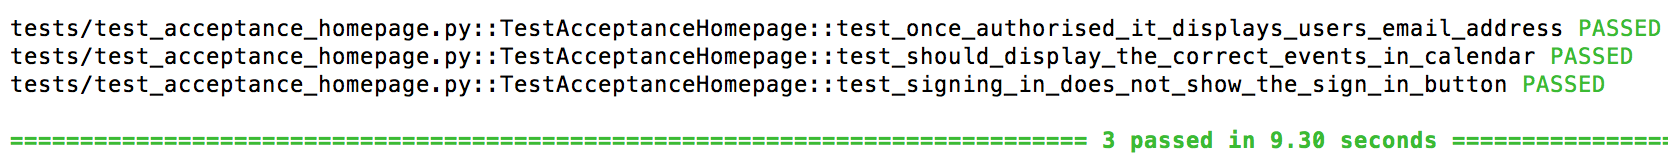
\includegraphics[width=\textwidth]{images/test_acceptance_homepage}
  \caption{Acceptance test being conducted for the homepage, to ensure that the homepage displays the correct content.}
  \label{fig:acceptance_homepage}
\end{figure}

\subsection{Calendar item}

\subsection{DateTimeHelper}


\section{Acceptance tests}
\label{appendix:acceptance}
The following section displays visual representation of the acceptance tests being executed, and their overall status.
\subsection{Homepage}

\begin{figure}[H]
  \centering
  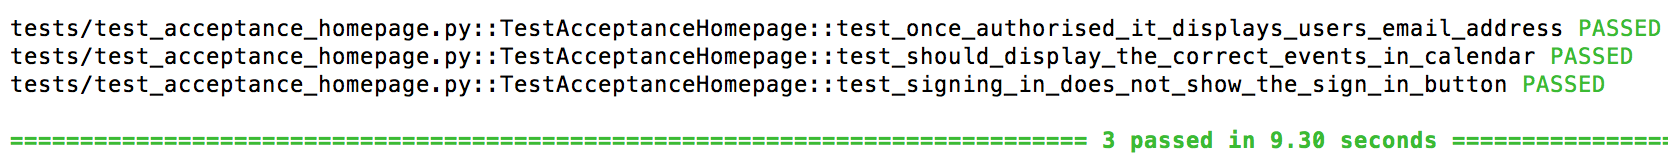
\includegraphics[width=\textwidth]{images/test_acceptance_homepage}
  \caption{Acceptance test being conducted for the homepage, to ensure that the homepage displays the correct content.}
  \label{fig:acceptance_homepage}
\end{figure}

\subsection{Add meta-data}

\begin{figure}[H]
  \centering
  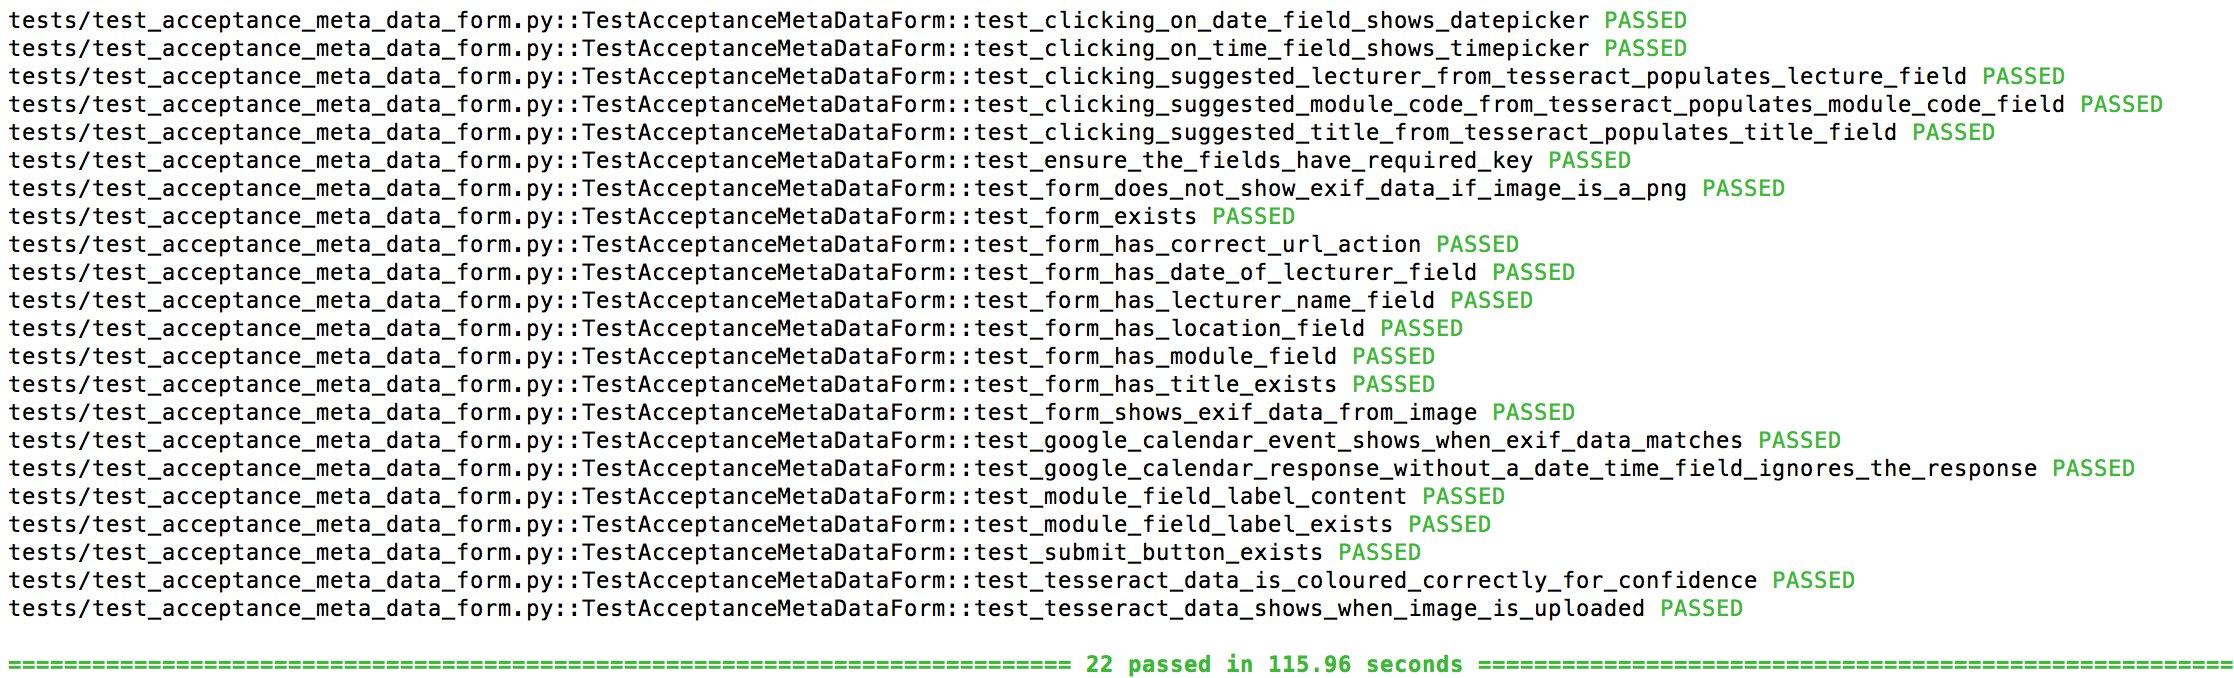
\includegraphics[width=\textwidth]{images/test_acceptance_meta_data_form}
  \caption{Acceptance test being performed to ensure that meta-data can be added to the correct note.}
  \label{fig:acceptance_add_meta_data}
\end{figure}

\subsection{Edit meta-data}
\begin{figure}[H]
  \centering
  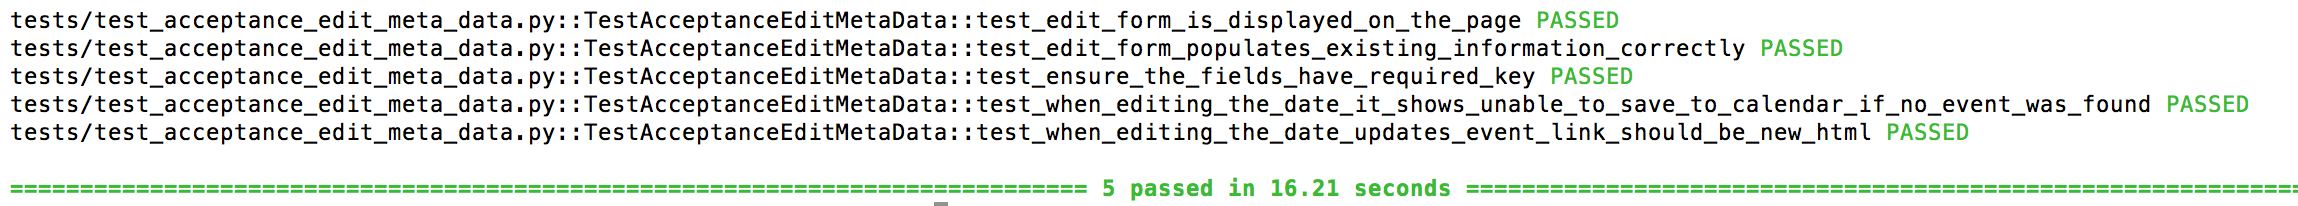
\includegraphics[width=\textwidth]{images/test_acceptance_edit_meta_data}
  \caption{Acceptance test being conducted so that a note's meta-data can be edited successfully.}
  \label{fig:acceptance_edit_meta_data}
\end{figure}
\subsection{Search}

\begin{figure}[H]
  \centering
  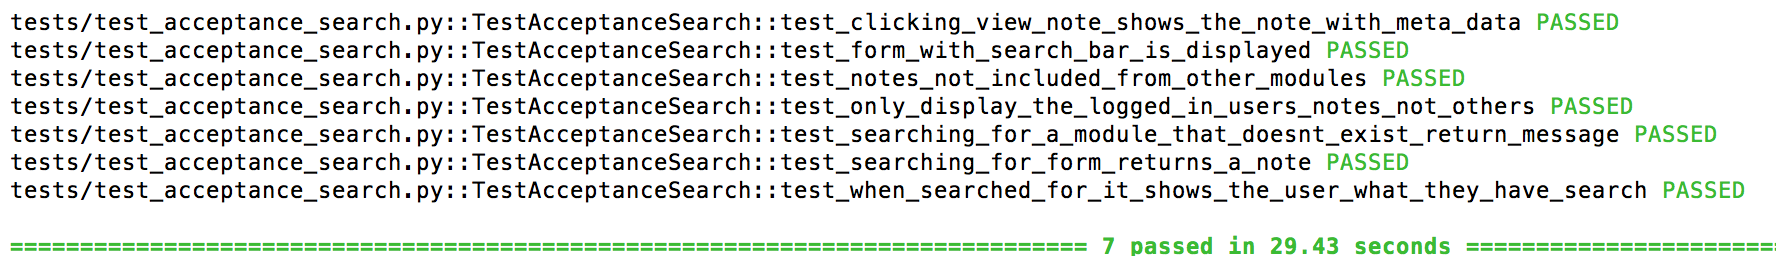
\includegraphics[width=\textwidth]{images/test_acceptance_search}
  \caption{Acceptance test to ensure that a user can search for a module code and it displays their notes.}
  \label{fig:search}
\end{figure}

\subsection{Viewing all the notes}

\begin{figure}[H]
  \centering
  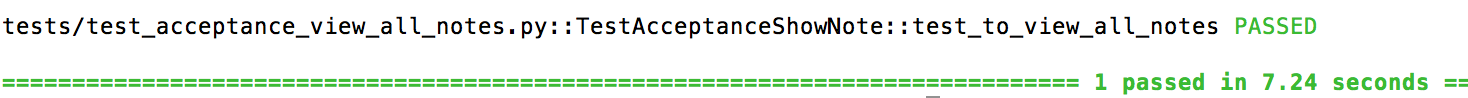
\includegraphics[width=\textwidth]{images/test_acceptance_view_notes}
  \caption{Acceptance test being conducted to ensure that all the notes can be viewed.}
  \label{fig:acceptance_view_note}
\end{figure}
\subsection{Show a note}

\begin{figure}[H]
  \centering
  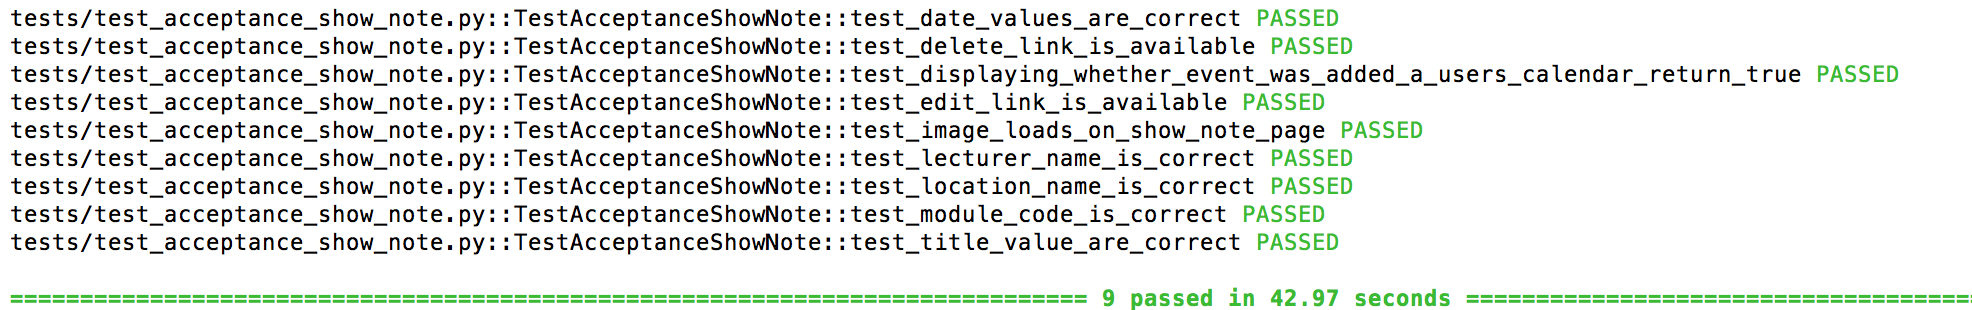
\includegraphics[width=\textwidth]{images/test_acceptance_show_note}
  \caption{Acceptance test being conducted to make sure that a singular note can be viewed correctly.}
  \label{fig:acceptance_homepage}
\end{figure}

\section{Integration tests}
\label{appendix:integration_tests}

\subsection{Add and edit meta data}
\begin{figure}[H]
  \centering
  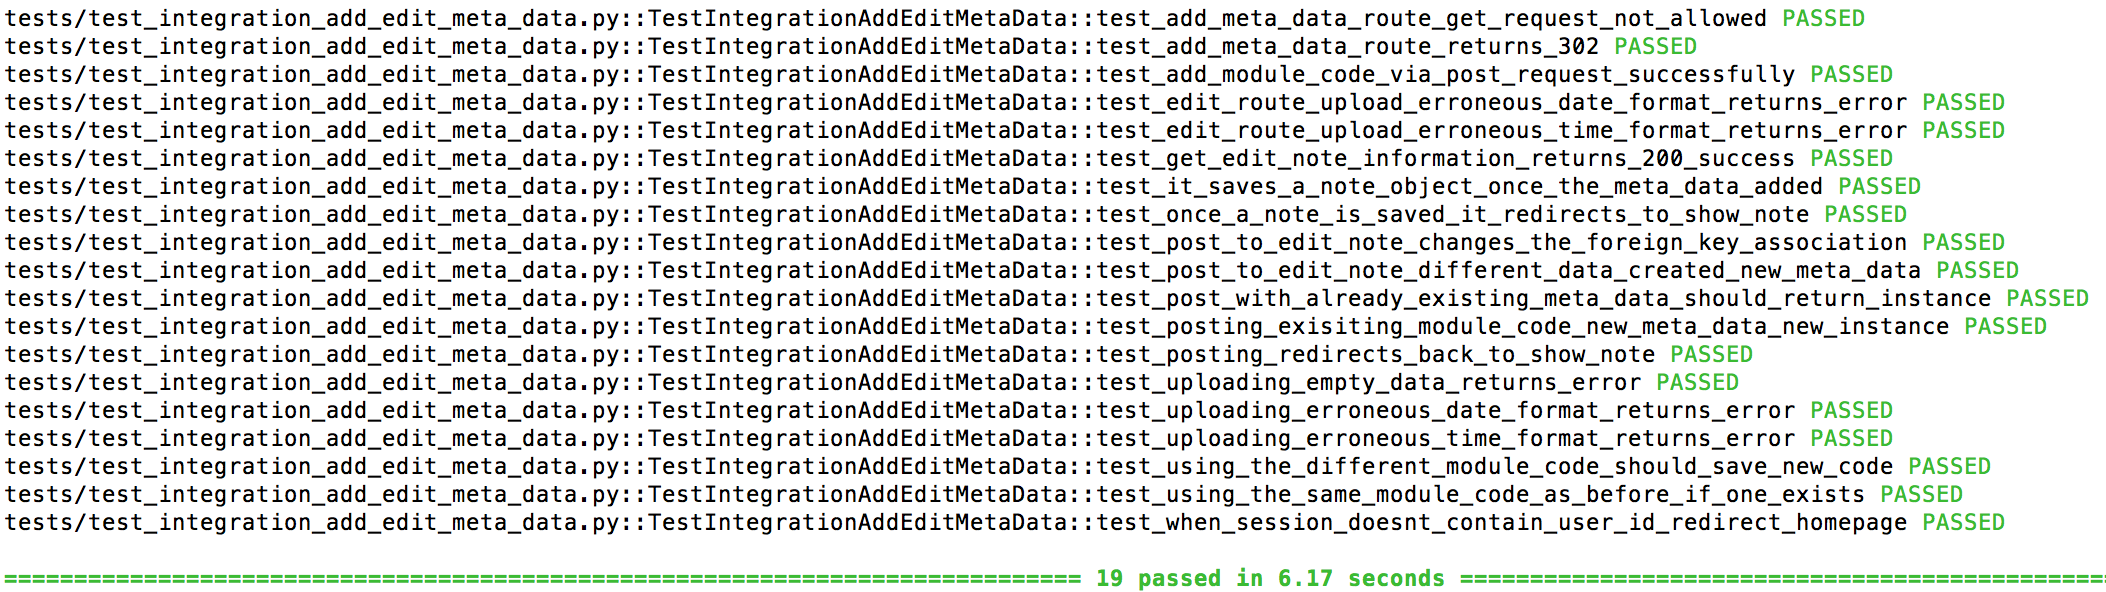
\includegraphics[width=\textwidth]{images/test_integration_add_edit_meta_data}
  \caption{Integration tests carried on the add and edit meta url to ensure the system worked well together.}
  \label{fig:integration_add_edit}
\end{figure}

\subsection{Homepage}
\begin{figure}[H]
  \centering
  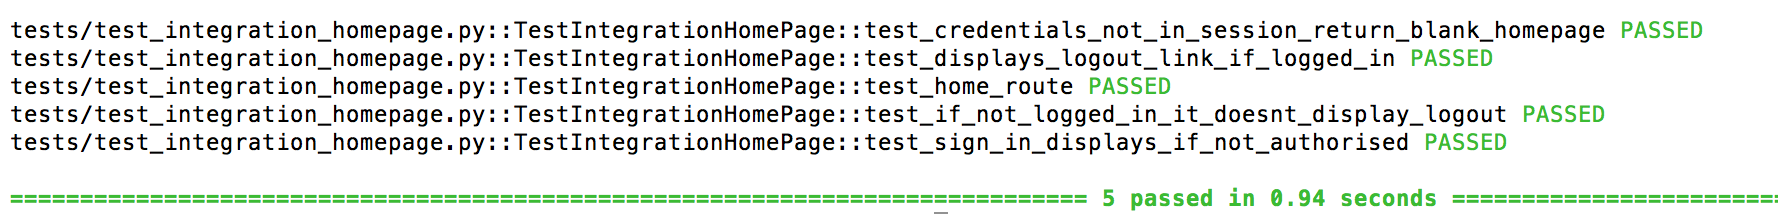
\includegraphics[width=\textwidth]{images/test_integration_homepage}
  \caption{Integration tests conducted on the homepage to ensure that the routes were accessible.}
  \label{fig:integration_homepage}
\end{figure}

\subsection{Logout}
\begin{figure}[H]
  \centering
  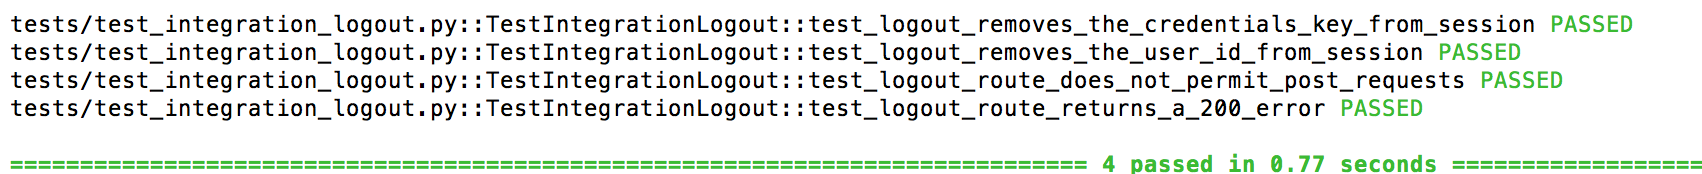
\includegraphics[width=\textwidth]{images/test_integration_logout}
  \caption{Integration tests conducted for the logout route ensuring the routes are logged out.}
  \label{fig:integration_logout}
\end{figure}

\subsection{Oauth}
\begin{figure}[H]
  \centering
  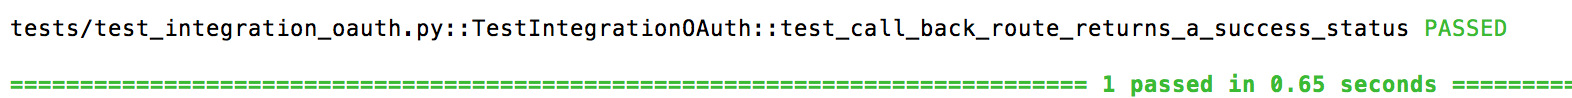
\includegraphics[width=\textwidth]{images/test_integration_oauth}
  \caption{Integration tests conducted for the oAuth route which interacts with the Google API.}
  \label{fig:integration_oauth}
\end{figure}

\subsection{Search}
\begin{figure}[H]
  \centering
  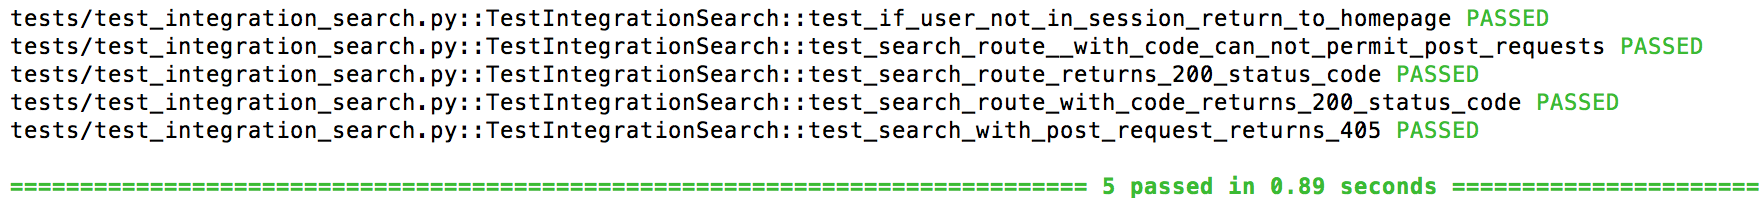
\includegraphics[width=\textwidth]{images/test_integration_search}
  \caption{Integration tests conducted for the search URL to ensure searching works correctly.}
  \label{fig:integration_search}
\end{figure}

\subsection{Show note}
\begin{figure}[H]
  \centering
  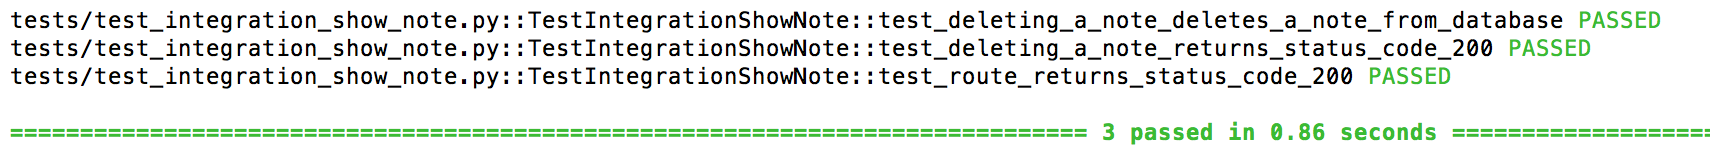
\includegraphics[width=\textwidth]{images/test_integration_show_note}
  \caption{Integration tests implemented to ensure that the note can be displayed properly. }
  \label{fig:integration_show_note}
\end{figure}

\section{Upload}
\begin{figure}[H]
  \centering
  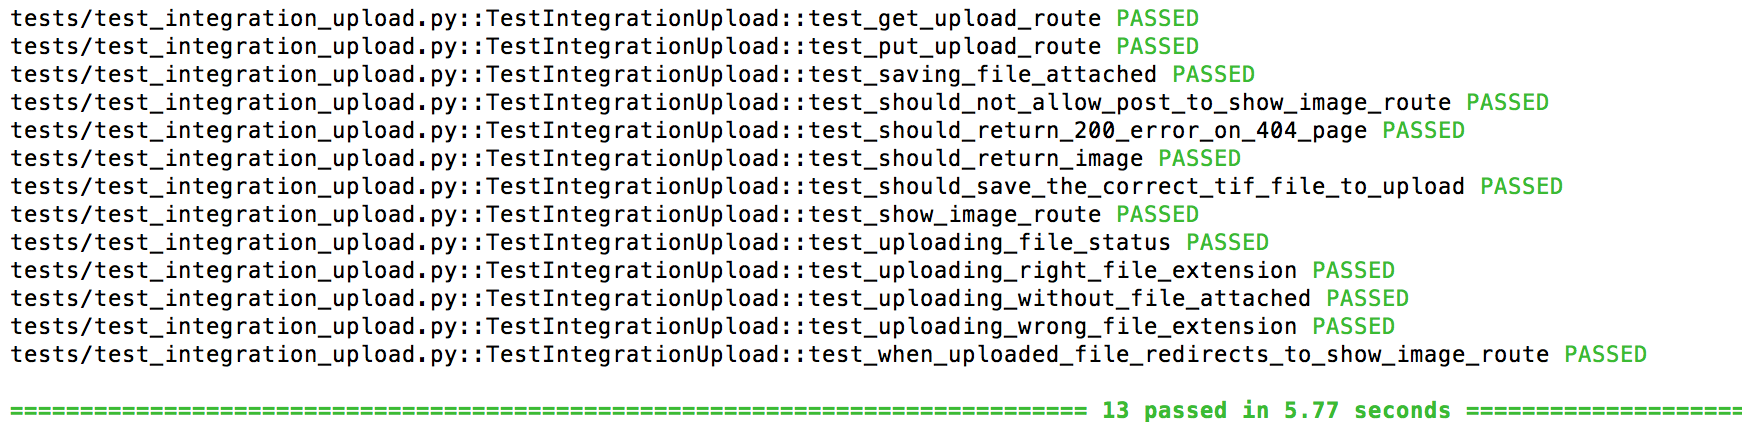
\includegraphics[width=\textwidth]{images/test_integration_upload}
  \caption{Integration tests implemented to ensure that a user can upload their images to the application. }
  \label{fig:integration_upload}
\end{figure}

\section{User}
\begin{figure}[H]
  \centering
  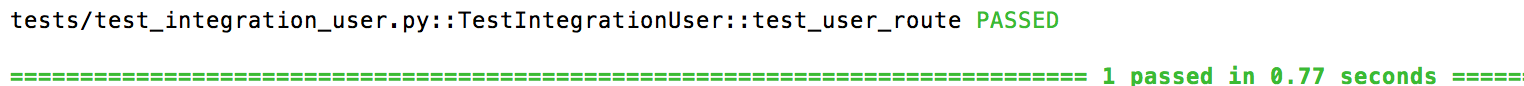
\includegraphics[width=\textwidth]{images/test_integration_user}
  \caption{Integration tests implemented the user route is working correctly and a the user gets added to the database.}
  \label{fig:integration_user}
\end{figure}

\section{View all notes}
\begin{figure}[H]
  \centering
  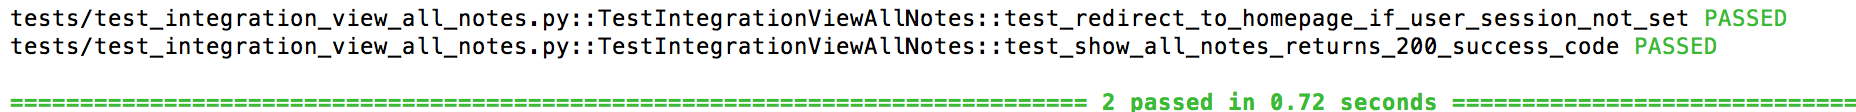
\includegraphics[width=\textwidth]{images/test_integration_view_all_notes}
  \caption{Integration tests to make sure the view all notes url is working and getting the appropriate notes from the database.}
  \label{fig:integration_view_all_notes}
\end{figure}


\section{User tests}

\chapter{Tesseract data results}
\label{appendix:tesseract}
This chapter shows the table outputting the results from the Tesseract training phase.

\section{Table}
\label{appendix:tesseract_table}

\begin{table}[h!]
\centering
 \begin{tabular}{||c c c c||}
 \hline
 Experiment & Characters Identified & Characters Correct & Correct Percentage \\ [0.5ex]
 \hline\hline
 1 & 114 & 70  & 61.40 \\
 2 & 252 & 182 & 72.22 \\
 3 & 345 & 280 & 81.15 \\
 4 & 335 & 265 & 79.10 \\
 5 & 288 & 201 & 69.79 \\
 6 & 276 & 206 & 74.63 \\
 7 & 326 & 256 & 78.52 \\
 8 & 400 & 279 & 69.75 \\
 9 & 462 & 364 & 78.78 \\
 10 & 401 & 266 & 66.33 \\
 11 & 366 & 240 & 65.57 \\
 12 & 362 & 273 & 75.41 \\ [1ex]
 \hline
 \end{tabular}
 \caption{A table which shows the statistics from the correctly identified characters during the training process.}
\end{table}

\chapter{Example test data}
%TC:ignore

\label{appendix:test_data}

\section{Calendar week response mock}
\begin{lstlisting}
  {
  "accessRole": "owner",
  "defaultReminders": [
    {
      "method": "email",
      "minutes": 30
    },
    {
      "method": "popup",
      "minutes": 30
    }
  ],
  "etag": "\"1234567891012345\"",
  "items": [
    {
      "kind": "calendar#event",
      "etag": "\"1234567891012345\"",
      "id": "ideventcalendaritem1",
      "status": "confirmed",
      "htmlLink": "https://www.google.com/calendar/event?testtest",
      "created": "2014-09-10T14:53:25.000Z",
      "updated": "2014-09-10T14:54:12.748Z",
      "summary": "Test Example",
      "creator": {
        "email": "test@gmail.com",
        "displayName": "Tester",
        "self": true
      },
      "organizer": {
        "email": "test@gmail.com",
        "displayName": "Test",
        "self": true
      },
      "start": {
        "dateTime": "2016-12-01T01:00:00+01:00"
      },
      "end": {
        "dateTime": "2016-12-01T02:30:00+01:00"
      },
      "transparency": "transparent",
      "visibility": "private",
      "iCalUID": "123456789@google.com",
      "sequence": 0,
      "guestsCanInviteOthers": false,
      "guestsCanSeeOtherGuests": false,
      "reminders": {
        "useDefault": true
      }
    }
  ],
  "kind": "calendar#events",
  "nextSyncToken": "synctokenasbebebe=",
  "summary": "test@gmail.com",
  "timeZone": "Europe/London",
  "updated": "2016-03-16T15:13:26.416Z"
}

\end{lstlisting}

\section{Google plus response mock}
\begin{lstlisting}
{
  "tagline": "Some Dummy data taglone",
  "verified": "False",
  "circledByCount": 100,
  "objectType": "person",
  "emails": [
    {
      "type": "account",
      "value": "test@gmail.com"
    }
  ],
  "occupation": "A Test Occupation"
}
\end{lstlisting}

\section{Google Oauth response} \label{oauth:response}
An excerpt from the oauth response
\begin{lstlisting}
{
  "access_token": "foo",
  "expires_in": 10,
  "refresh_token": "refresh"
}
\end{lstlisting}
%TC:endignore 

\chapter{Image Processing}
%TC:ignore

\label{appendix:image_processing}

\section{Pre-blue lined image}
\label{processing:pre-line}
\begin{figure}[H]
  \centering
  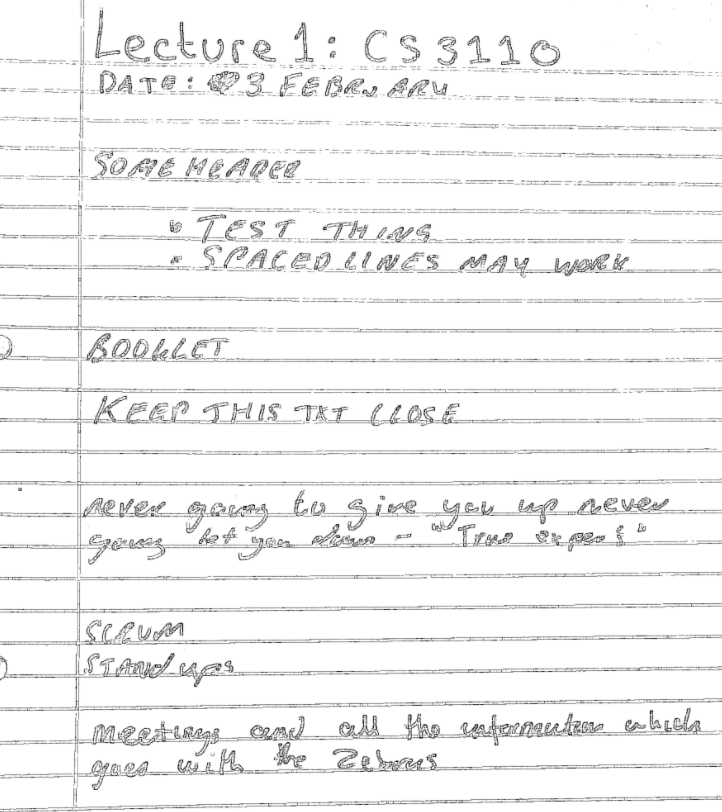
\includegraphics{images/pre-line-editing}
  \caption{The adaptive threshold on normal lined paper caused too much noise to be interfered with the Tesseract engine}
  \label{fig:pre-line-editing}
\end{figure}

\section{Filtering the blue lines}
\label{processing:filter_blue}
\begin{figure}[H]
  \centering
  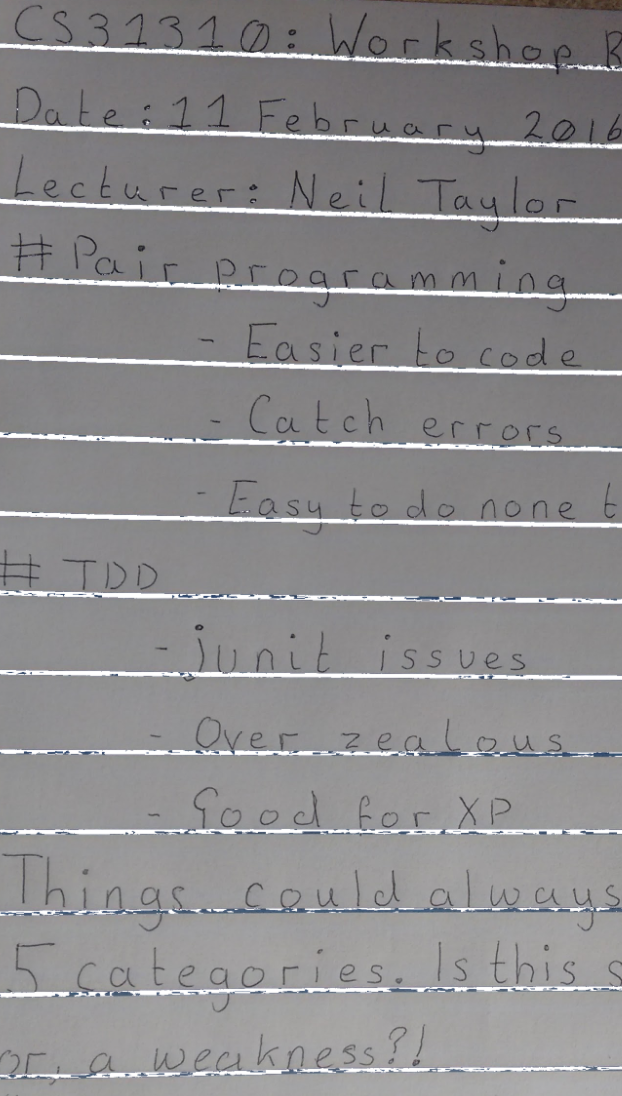
\includegraphics{images/blue_identified}
  \caption{Blue lines in the adaptive threshold have been identified and removed to be a white colour.}
  \label{fig:blue-identified}
\end{figure}
%TC:endignore 

\chapter{Design decisions}
\label{appendix:design}

\section{Class diagram}
\label{design:class_diagram}
%\begin{figure}[H]
  \begin{sidewaysfigure}
    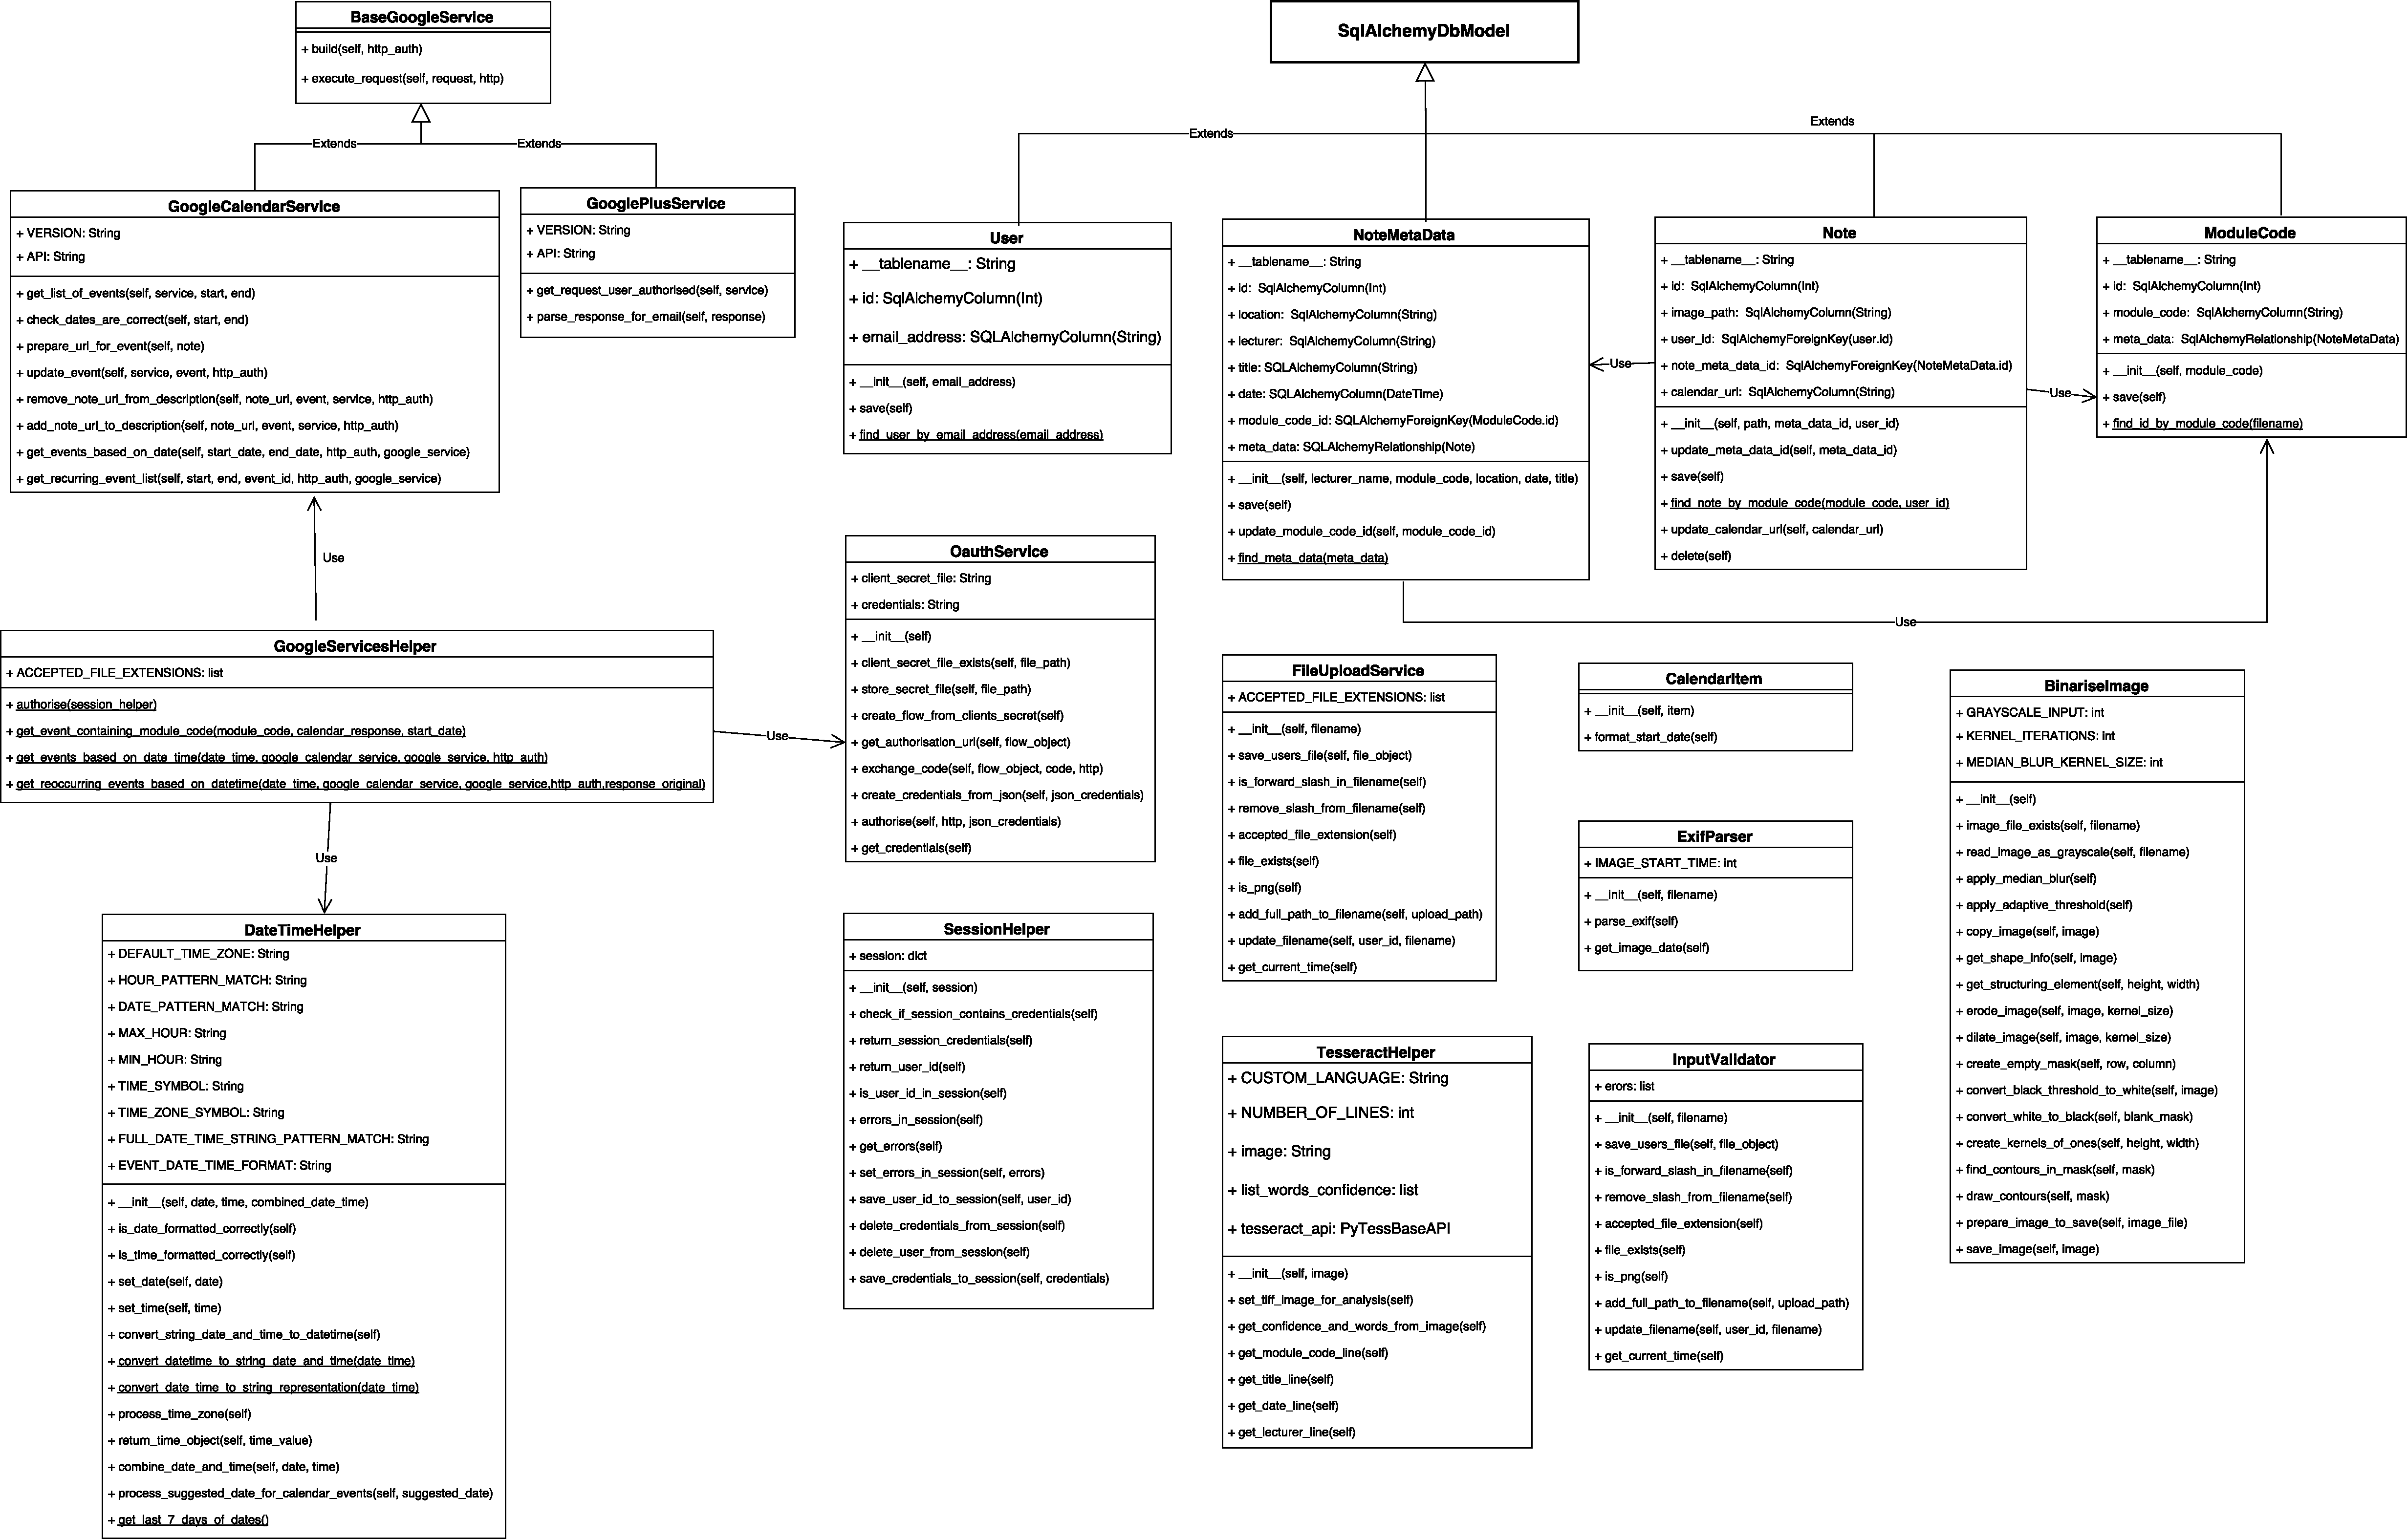
\includegraphics[scale=0.3]{images/class_diagram.pdf}
    \caption{The overall class diagram of the models directory, not including the controllers}
  \end{sidewaysfigure}
  %\centering
  %\includegraphics[scale=0.3]{images/class_diagram}
  %\label{fig:class_diagram}
  %\caption{The overall class diagram of the models directory, not including the controllers}
%\end{figure}

\section{CRC cards}
Below is an excerpt of the the examples of a more complex CRC card design in the system. Throughout the the project, each class went through an iterative process of using CRC cards. Therefore, a lot of them have been omitted to save space.

\begin{figure}[H]
  \centering
  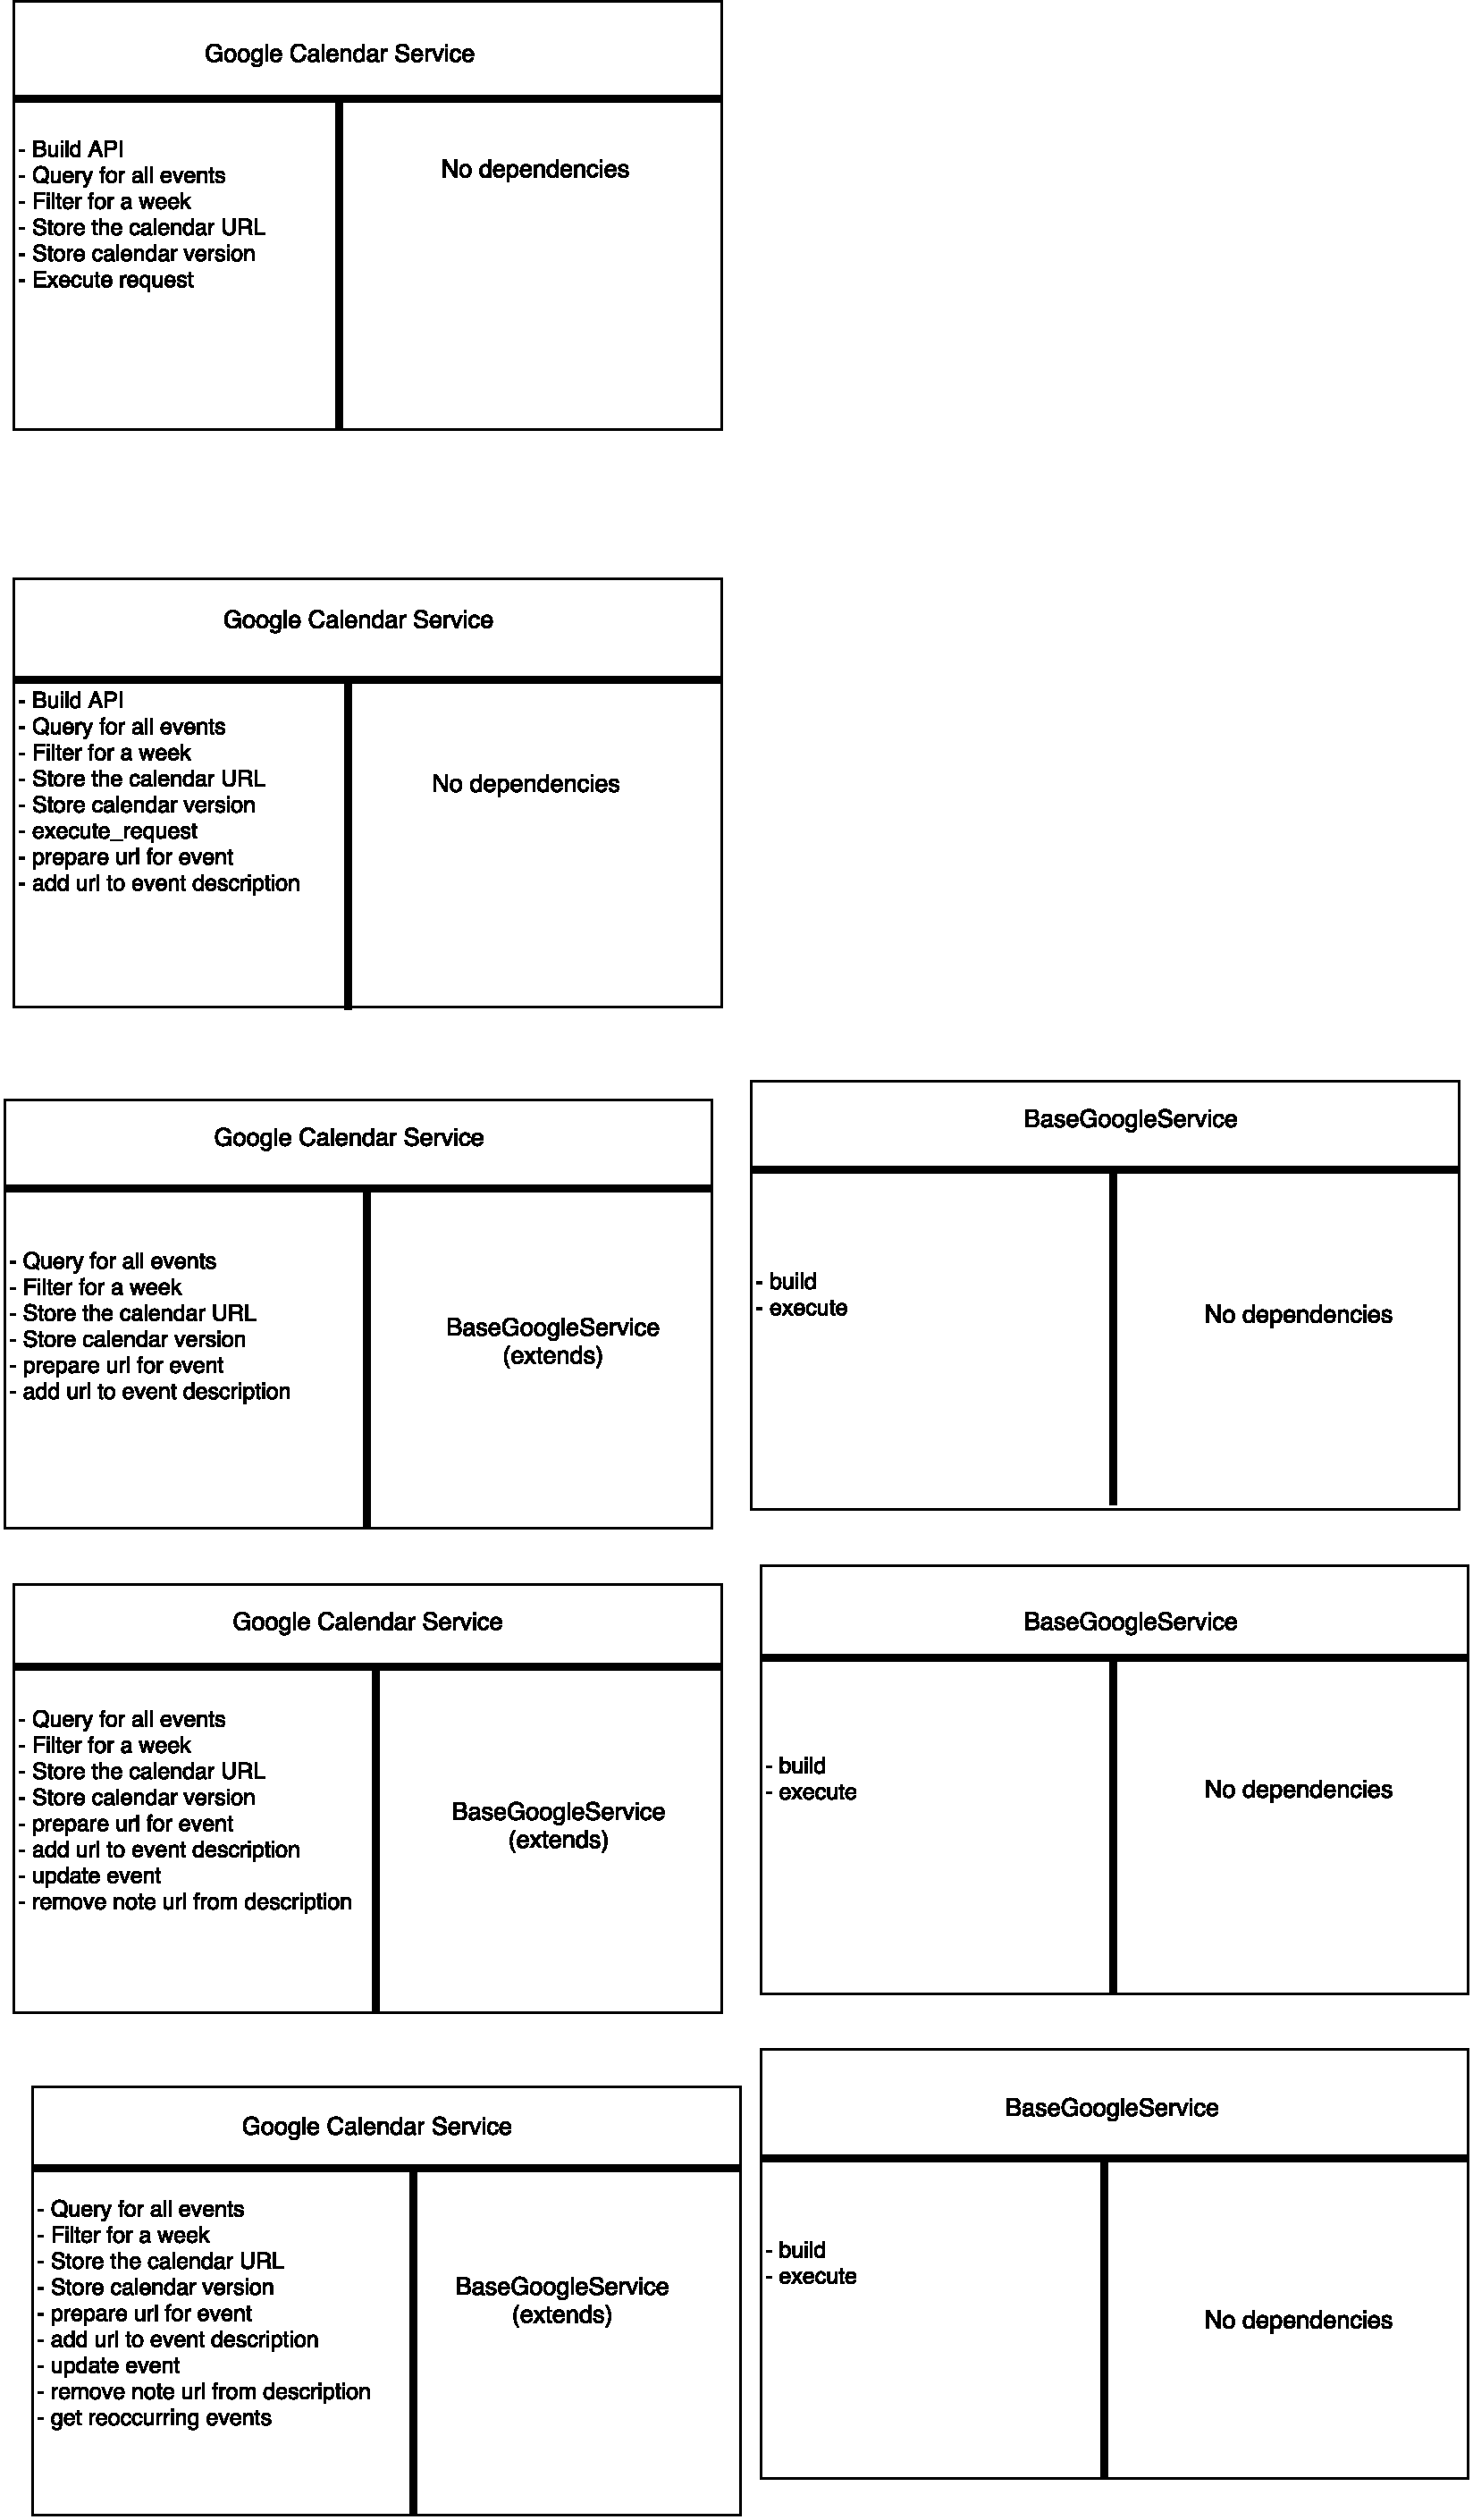
\includegraphics{images/google_calendar_service.pdf}
  \label{fig:crc_card_google_calendar}
  \caption{An iterative approach to the CRC cards, used in the design of the Google calendar service. Each now card represents a new state in which the system has evolved.}
\end{figure}

\chapter{Scrum process supplementary materials}
%TC:ignore
The appendix discusses some of the additional material to show the process of scrum used as the methodology of choice.
Below is a collection of user-stories throughout the sprints.
\section{Sprint burndown charts}
\begin{figure}[H]
  \centering
  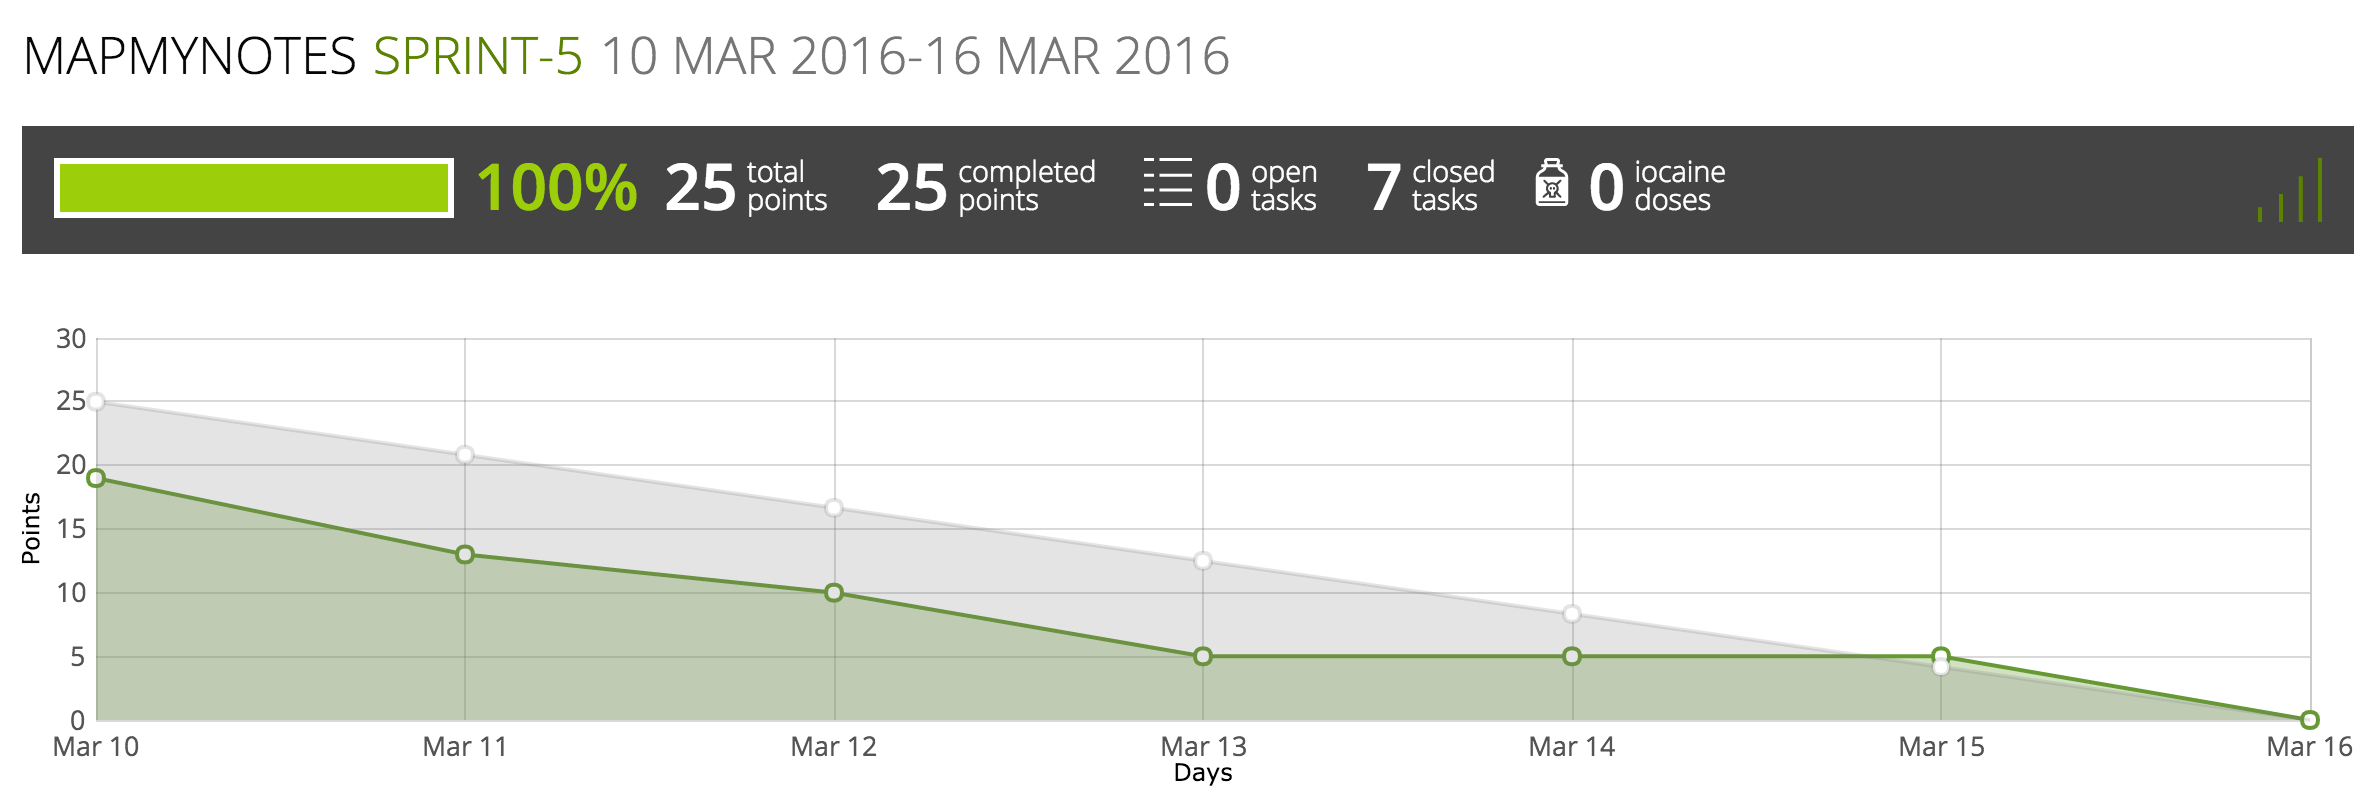
\includegraphics[scale=0.35]{images/sprint-5-burndown-chart}
  \caption{An example of the burndown chart for a sprint, showing areas where there may have been difficulty.}
  \label{fig:sprint-burndown}

\end{figure}

\section{Overall burndown chart}
\begin{figure}[H]
  \centering
  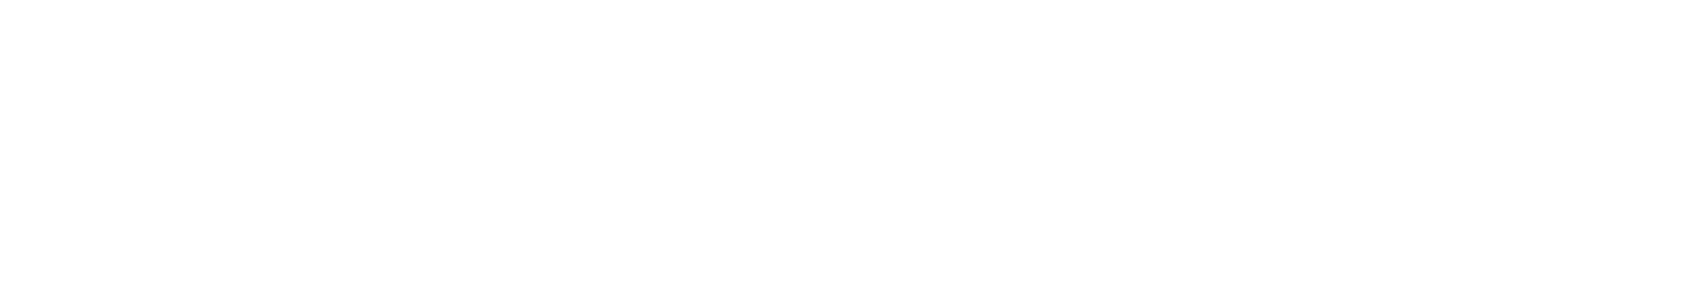
\includegraphics[scale=0.5]{images/overall-burndown}
  \caption{The overall burndown of the sprints during the development period. This clearly shows a consistent work flow up until more knowledge of the project was achieved, going below the expectation line.}
  \label{fig:overall_burndown}
\end{figure}

\begin{table}[h!]
\centering
\begin{tabular}{|p{1cm} p{10cm} p{1cm} p{1cm}|}
   \hline
 Id & User story & Sprint & Story points \\ [0.5ex]
 \hline\hline
 1 & As a user I want to be able to upload an image of a set of notes so that I can see my note in the application & 2	& 10 \\
 2 & As a user I want to be able to tag my notes so that  all my notes are under the correct module	& 4	 & 5 \\
 3&As a user I want to be able to add information about the notes so that I can reference them in the future&4&15 \\
 4&As a user I want to be able to save a note, so that I can find it again later&3&10 \\
 5&As a user I want to be able to search for a given module, so that I can find all notes for that module&7&8 \\
 6&As a user I want to be able to sign in via google sign in&5&15 \\
 7&As a user I want to use Tesseract OCR so that I can identify characters&1&15 \\
 8&As a user I want to be able to view the application on a website&2&5 \\
 9&As the customer I want to see the image being binarised properly&2&10 \\
 10&As a developer I need to train my handwriting, so that Tesseract can recognise my handwriting&10&n/a \\
 11&As a user I want to be able to edit the meta data, so that I can update it in light of a change&5&5 \\
 12&As a user I want to be able to remove a note incase I do not want it to appear&5&5 \\
 13&As a developer I want to the website to have good styling&4&8 \\
 14&As a developer I want to integrate tesseract into the application, so it can read information from a note&8&8 \\
 15&As a user I want to be able to view all the notes I have as a user so I can easily find all of them again&6&3 \\
 16&As a user I want to view a list of events on the homepage from my calendar, so I can see recent events&6&15 \\
 17&As a user I want to be able to save the URL in the calendars event&7&10 \\
 18&As a user I want to be able to tag the title of the lecture, so that I can know which one it is.&6&5 \\
 19&As a user, when I authorise I want to show my email address and remove the authorise button, so I know I have signed in&6&3 \\
 20&As a developer I want to be able to get the date taken from EXIF data, to show information about a note&7&8 \\
 21&As a user I want to be able to edit the date and update my calendar&9&8 \\
 22&As a developer I want to be able to associate a note with a user&7&5 \\
 23&As a user, I want to be able to have automated suggestion of meta data from the image, so that I can know what to tag.&8&5 \\
 24&As a user, I want to be able to logout, so that I can close my session&8&5 \\
 25&As a user I want to be able to click Tesseract Items, so that it's easier for me to put in the fields.&9&10 \\
 26&As a user I want to be able to edit and save to reoccurring events&10&10 \\
 \hline
 \end{tabular}
 \caption{A table showing the user stories identified throughout the project, along with the sprint in which they were implemented and associated story points}
\end{table}
%TC:endignore

\fancypagestyle{plain}{%
   \fancyhead{} %[C]{Annotated Bibliography}
   \fancyfoot[C]{{\thepage} of \pageref{LastPage}} % except the center
   \renewcommand{\headrulewidth}{0pt}
   \renewcommand{\footrulewidth}{0pt}
}

\setemptyheader

\nocite{*} % include everything from the bibliography, irrespective of whether it has been referenced.

% the following line is included so that the bibliography is also shown in the table of contents. There is the possibility that this is added to the previous page for the bibliography. To address this, a newline is added so that it appears on the first page for the bibliography.
\addcontentsline{toc}{chapter}{Annotated Bibliography} % Adds References to contents page

%
% example of including an annotated bibliography. The current style is an author date one. If you want to change, comment out the line and uncomment the subsequent line. You should also modify the packages included at the top (see the notes earlier in the file) and then trash your aux files and re-run.
%\bibliographystyle{authordate2annot}
\bibliographystyle{IEEEannot}
\renewcommand{\bibname}{Annotated Bibliography}
\bibliography{References/references} % References file


\end{document}
